% Modulo de vision por computadora
\section{Visión por computadora} 

Con el fin de cumplir con los objetivos generales y específicos del proyecto, se definió una metodología compuesta por seis etapas, cada una con objetivos claramente definidos.  
La primera de estas consistió en delimitar el universo de palabras que se utilizaría para entrenar el modelo, buscando palabras de uso cotidiano que permitieran crear una gran cantidad de frases con un alto nivel de utilidad.  
Una vez definido el universo de palabras, se procedió con la recopilación de datos, la cual incluyó crear un conjunto de datos con videos de las señas correspondientes a las diferentes palabras que se utilizarían.  
El siguiente paso consistió en preparar el conjunto de datos con los videos recopilados anteriormente, lo cual mayormente consistió en identificar manualmente cada señal para que estos datos pudieran ser utilizados en el proceso de entrenamiento.  
Al tener listo el conjunto de videos, se pudo proceder al procesamiento de las imágenes, el cual se realizó con la librería Mediapipe de Google, que creó esqueletos de los movimientos capturados en los diferentes videos.  
Este esqueleto se utilizó para entrenar una red neuronal que fuera capaz de identificar las diferentes señas del universo de palabras seleccionado.  
Como último paso, se evaluó el desempeño del modelo, buscando áreas de mejora.  

\subsection{Delimitación del universo de palabras}
Dada la restricción de tiempo para la finalización del proyecto, resultó esencial establecer un conjunto definido de palabras que se emplearían en el entrenamiento y la evaluación del modelo.
La selección de las palabras que formaron parte de este universo fue extremadamente importante para la utilidad del proyecto, ya que elegir las palabras equivocadas pudo haber significado que el proyecto no cumpliera con los objetivos establecidos.
Para este proceso, se seleccionaron al menos veinticinco palabras que en conjunto se pudieran utilizar para crear una gran cantidad de frases de uso cotidiano.
La primera fase de este proceso requirió de alguien con amplio conocimiento de la lengua de señas de Guatemala, y consistió en identificar al menos cincuenta palabras que se utilizaran con frecuencia.
Al tener este dato inicial, se analizó cuáles de estas palabras se podrían utilizar para formar oraciones congruentes, haciendo énfasis en la utilidad y frecuencia de uso de estas.
Adicionalmente, se tomó en cuenta el grado de similitud de la seña con las demás palabras del universo de palabras. Esto con el objetivo de reducir la probabilidad de que el modelo confundiera dos señas diferentes debido a que eran muy similares.

Al finalizar la lista original de palabras, se buscó retroalimentación de las personas que ayudaron con la grabación de los videos de entrenamiento.
Este paso fue crucial para asegurar que las palabras seleccionadas fueran relevantes y útiles en el contexto de la lengua de señas de Guatemala.
Las opiniones de los colaboradores permitieron identificar posibles mejoras en la selección de palabras y garantizar que el conjunto final reflejara adecuadamente las necesidades de los usuarios.
Tomando en cuenta la retroalimentación recibida, se ajustó por una última vez la lista de palabras para asegurar que el universo de palabras seleccionado fuera el más adecuado para el proyecto.

\subsection{Recopilación de datos}
Al tener un universo de palabras claramente definido, se pudo proceder a recopilar los datos necesarios para representar todas las palabras elegidas.  
En esta fase del proyecto, nuevamente se requirió del apoyo de una persona con un profundo conocimiento de la lengua de señas de Guatemala para crear los videos que servirían como base del conjunto de datos.  
Para que el modelo contara con una amplia variedad de datos de entrenamiento, se realizaron quince tomas de cada seña que formara parte del universo de palabras.  
Se utilizaron tres ángulos de cámara diferentes, de frente y vista en diagonal de cada lado, realizando cinco tomas desde cada uno de los ángulos.  
El objetivo de utilizar diferentes ángulos fue mejorar la habilidad del modelo para reconocer las señas en condiciones no ideales, ya que no se podía esperar que el usuario siempre estuviera perfectamente alineado a la cámara.  
De igual manera, el objetivo de realizar cinco tomas desde cada uno de los ángulos fue que el modelo pudiera identificar las señas correctamente a pesar de las ligeras variaciones que se pudieran presentar en los movimientos.  

Al tomar estos videos, se buscó que el usuario que realizara las señas lo hiciera de forma clara y precisa, evitando movimientos innecesarios que pudieran confundir al modelo.
Adicionalmente, se tuvo cuidado de que el fondo de los videos fuera lo más simple posible, para asegurar que MediaPipe pudiera identificar correctamente las manos del usuario.
Durante esta fase del proyecto se realizo el hallazgo de que las personas surdas realizan las señas de forma diferente, por lo que se tuvo que tomar en cuenta este factor al momento de grabar los videos.

\begin{figure}[H]
    \centering
    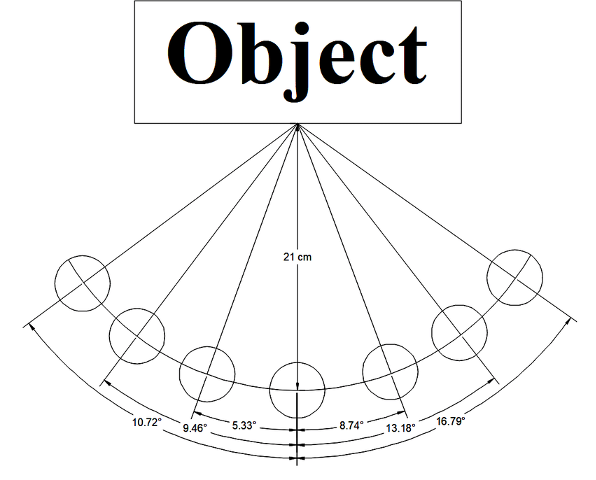
\includegraphics[width=0.7\textwidth]{figuras/Angles.png}
    \caption{Ejemplos de captura de los videos para el conjunto de datos. \cite{kucsvan2019}.}
    \label{fig:angulos}
\end{figure}


\subsection{Preparación del conjunto de datos}
Después de recopilar los datos que formaron parte del conjunto de datos, se procedió con la creación de este.  
El primer paso para preparar el conjunto de datos fue identificar correctamente todos los videos que se tomaron en el paso anterior.  
Para esto, nuevamente se requirió de la asistencia de alguien con conocimiento de la lengua de señas de Guatemala, ya que cualquier error llevaría a que el modelo identificara erróneamente las señas.  
La identificación de los videos se realizó por medio del nombre del archivo, el cual siguió el siguiente formato: {Seña}-{Vista}-{Toma}.  
El valor de “vista” fue \textit{Frente}, \textit{Der}, o \textit{Izq}, para indicar si el video se tomó con una vista frontal, o una vista lateral desde la izquierda o la derecha, el valor de “seña” indicó la palabra a la que corresponde el video, y el valor de “toma” indicó el número de toma que se realizó. 
Combinado con el valor de “toma”, se pudieron distinguir claramente los videos entre sí, lo cual resultó útil si el modelo terminó teniendo problemas para identificar la seña en un video en específico.  

Tomando en cuenta el hallazgo de que las personas surdas realizan las señas de forma diferente, se tuvo que tomar en cuenta este factor al momento de preparar el conjunto de datos.
Para garantizar que el modelo pudiera identificar las señas correctamente, se reflejaron los videos sobre el eje vertical, de forma que las señas realizadas por una persona zurda se vieran como si fueran realizadas por una persona diestra, y viceversa.
Esto permitió que el modelo pudiera identificar las señas de forma correcta sin importar si el usuario era zurdo o diestro.

\begin{figure}[H]
    \centering
    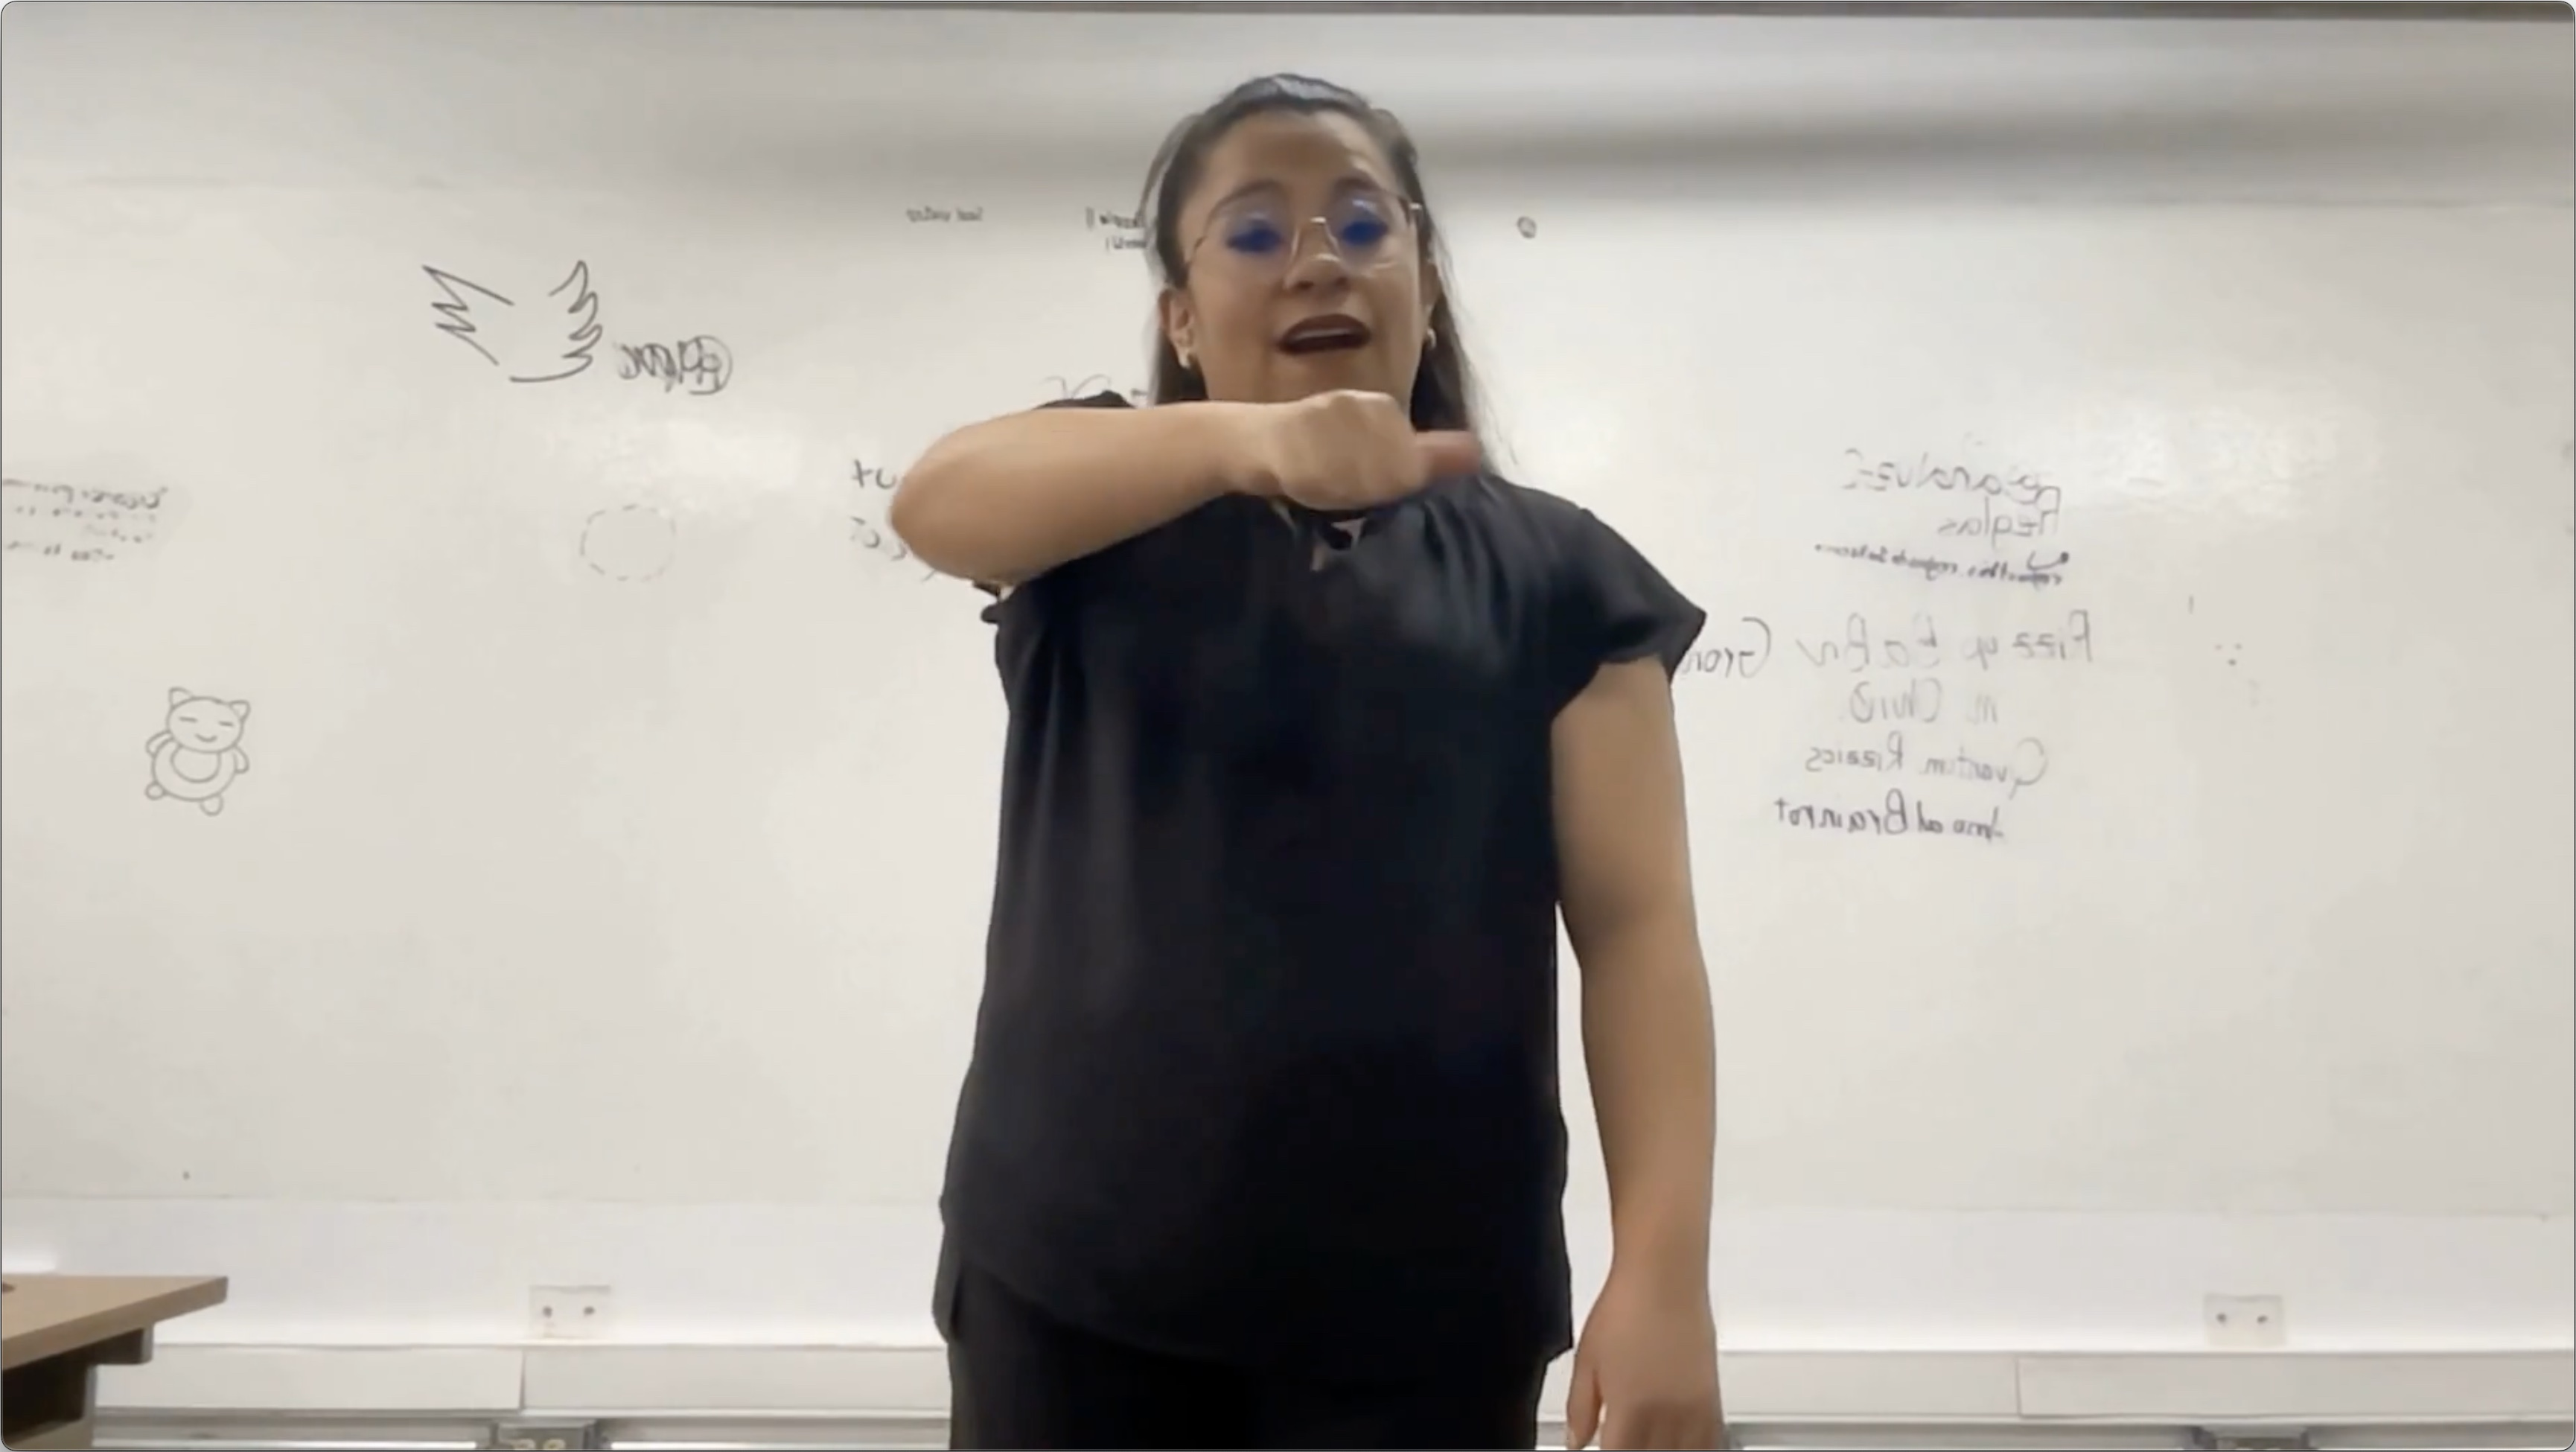
\includegraphics[width=0.9\textwidth]{figuras/EjemploVideo.jpeg}
    \caption{Ejemplo de reflejo de un video.}
    \label{fig:reflejo}
\end{figure}

\subsection{Procesamiento de los videos}

\begin{figure}[H]
    \centering
    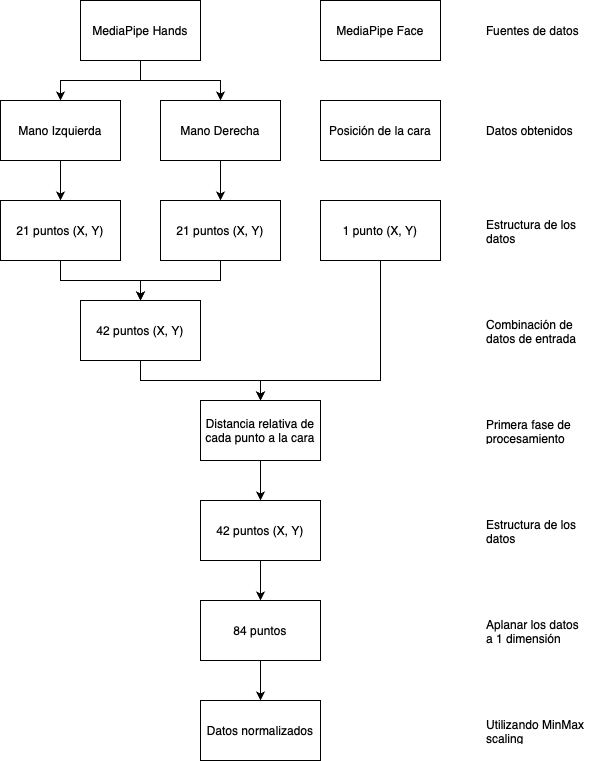
\includegraphics[width=0.85\textwidth]{figuras/DataPipeline.png}
    \caption{Proceso de preparación del conjunto de datos.}
    \label{fig:dataset_pipeline}
\end{figure}

Con el conjunto de datos ya definido, se pudo procesar los videos para crear datos que resultaran útiles para entrenar y validar el modelo.  
Para esto, se utilizó la librería MediaPipe de Google, la cual permite realizar el reconocimiento de manos en tiempo real.  
Esta librería utiliza modelos de aprendizaje automático para detectar y seguir la posición de las manos en imágenes o videos, ofreciendo información detallada sobre la mano, incluyendo la detección de puntos clave y gestos.  
Utilizando esta librería, se crearon esqueletos que representaron los movimientos capturados en cada video. 

\begin{figure}[H]
    \centering
    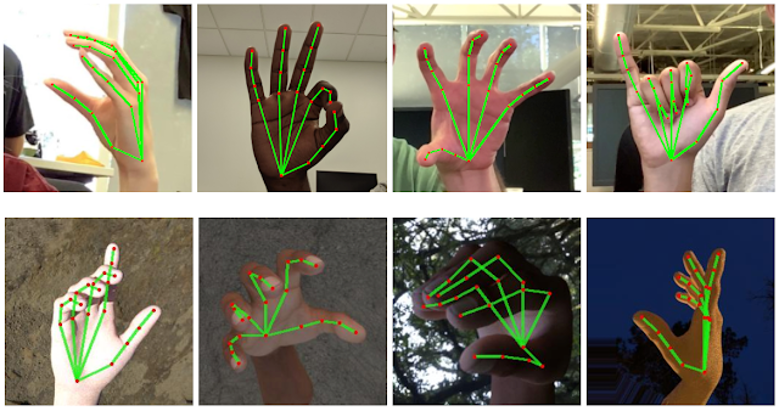
\includegraphics[width=0.7\textwidth]{figuras/Mediapipe.png}
    \caption{Ejemplo de uso de MediaPipe \cite{mediapipe}.}
    \label{fig:mediapipe uso}
\end{figure}

Utilizando estos esqueletos, se creó un conjunto de datos con todas las coordenadas relevantes para poder entrenar el modelo.
La librería MediaPipe detecta un total de veintiún puntos clave en cada mano, para un total de cuarenta y dos puntos clave por cada fotograma de video.
Debido a que en LENSEGUA la posición de las manos también es relevante, se decidió calcular la posición relativa de cada punto clave con respecto a la cara, procesando las coordenadas en X y Y de cada punto clave.
Cada uno de estos puntos cuenta con coordenadas en el eje x y en el eje y, lo cual resulta en un total de ochenta y cuatro características por fotograma de video.

\subsection{Labeling de los datos}
Después de procesar los videos y obtener las coordenadas de los puntos clave, se procedió a etiquetar los datos para que pudieran ser utilizados en el entrenamiento del modelo.
Esto consistió en asignar una etiqueta a cada fotograma de video, indicando la seña correspondiente a la palabra que se estaba realizando en ese fotograma.
Para esto, se utilizó la función to\_categorical de la librería Keras de Python, la cual convierte un vector de etiquetas en una matriz binaria.
Esta matriz binaria se utilizó para entrenar el modelo, permitiendo que este pudiera identificar las señas de la lengua de señas de Guatemala.
Es importante mencionar que, para que las predicciones del modelo se puedan interpretar de forma correcta, se creó un diccionario que relaciona cada etiqueta con la palabra correspondiente.

\subsection{Normalización de los datos}

Para permitir que el modelo pudiera identificar las señas de forma en tiempo real, los datos se procesaron de forma que cada fotograma de video se convirtiera en una secuencia de datos que representara el movimiento de las manos.
Tomando esto en cuenta, el conjunto de datos resultante consistió en una serie de secuencias de datos, cada una representando un fotograma de video y las coordenadas de los puntos clave detectados en ese fotograma.
Después de calcular estas características, se procedió a normalizarlas para que todas las características tuvieran un valor entre menos uno y uno.
Debido a que las coordenadas de los puntos clave podían ser negativas, para indicar que se encontraban a la izquierda o arriba de la cara, se utilizaron dos fórmulas diferentes para normalizar las coordenadas positivas y negativas.

Ecuación para normalizar coordenadas positivas:
\begin{equation}
    x_{norm} = \frac{x}{\left| x_{min} \right|}
\end{equation}

Ecuación para normalizar coordenadas negativas:
\begin{equation}
    x_{norm} = \frac{x}{\left| x_{max} \right|}
\end{equation}

Donde $x_{norm}$ es el valor normalizado de la coordenada $x$, $x$ es el valor de la coordenada $x$ original, $x_{min}$ es el valor mínimo de la coordenada en el conjunto de datos y $x_{max}$ es el valor máximo de la coordenada en el conjunto de datos.
Estas fórmulas se utilizaron para normalizar las coordenadas de los puntos clave en el eje x y en el eje y, lo cual permitió que todas las características tuvieran un valor entre -1 y 1.
El resultado de este proceso fue un conjunto de datos con las características normalizadas, las cuales se utilizaron para entrenar el modelo.
A continuación, se muestra un ejemplo de cómo se veían los datos después de ser procesados.

\begin{figure}[H]
    \centering
    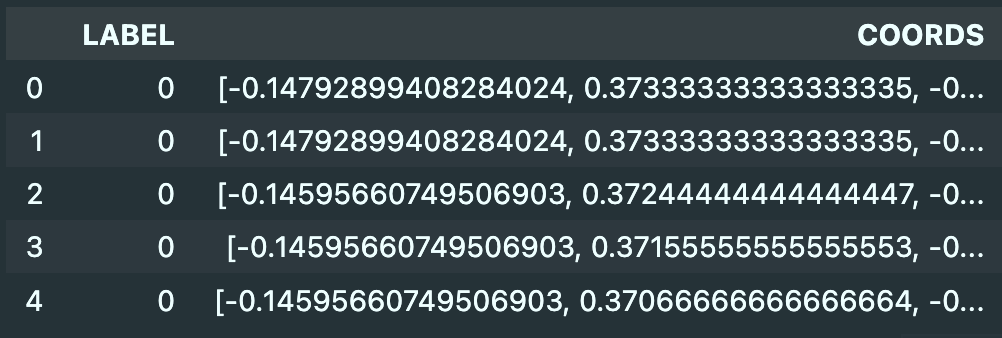
\includegraphics[width=0.7\textwidth]{figuras/ProccessedData.png}
    \caption{Ejemplo de datos procesados.}
    \label{fig:processed_data}    
\end{figure}

\subsection{Oversampling}
Debido al tamaño limitado del conjunto de datos, se utilizó la técnica de oversampling para aumentar la cantidad de datos disponibles para el entrenamiento del modelo.
Esta técnica consistió en duplicar los datos existentes, lo cual permitió que el modelo pudiera entrenarse con una mayor cantidad de datos y mejorar su capacidad para identificar las señas de la lengua de señas de Guatemala.
El oversampling se realizó copiando los datos existentes y agregando ruido a las coordenadas de los puntos clave, lo cual permitió que el modelo pudiera generalizar mejor a datos no vistos previamente.
Con cada uno de los modelos entrenados, se evaluó el desempeño del modelo utilizando el conjunto de datos original y el conjunto de datos aumentado, lo cual permitió determinar si el oversampling había mejorado la capacidad del modelo para identificar las señas.

\subsection{Entrenamiento del modelo}
Para entrenar el modelo, se utilizó el 80\% del conjunto de datos procesado en la fase anterior, mientras que el 20\% restante se utilizó para validar el modelo.
Durante este proceso, se probaron diferentes hiperparámetros y técnicas de entrenamiento para encontrar la combinación que ofreciera el mejor desempeño.
Adicionalmente, una vez seleccionada una red neuronal, se evaluó el desempeño de esta de forma continua para poder hacer ajustes y optimizaciones que mejoraran sus resultados.  

Debido a la naturaleza de los datos, se decidió utilizar una red neuronal \textit{feedforward} para entrenar el modelo.
Este modelo se utilizó para entrenar un clasificador que pudiera identificar las señas de la lengua de señas de Guatemala utilizando los datos procesados en la fase anterior.
En cada iteración, se ajustaron los hiperparámetros de la red neuronal, como el número de capas, el número de neuronas por capa y la tasa de aprendizaje, con el objetivo de mejorar la precisión del modelo.
Adicionalmente, se probaron diferentes funciones de activación y optimizadores para encontrar la combinación que resultara en el mejor desempeño.

\begin{figure}[H]
    \centering
    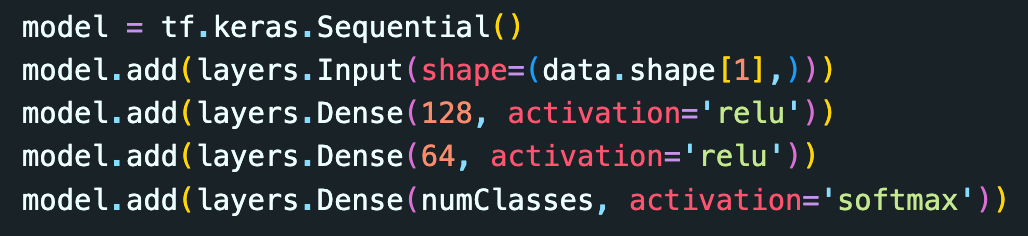
\includegraphics[width=0.7\textwidth]{figuras/FNN.png}
    \caption{Ejemplo de una red neuronal \textit{feedforward} sencilla.}
    \label{fig:feedforward}
\end{figure}

Con el objetivo de mejorar la capacidad del modelo para generalizar a datos no vistos previamente, se utilizó la técnica de \textit{dropout} durante el entrenamiento.
Esta técnica consistió en desactivar aleatoriamente un porcentaje de las neuronas en cada iteración, lo cual permitió que el modelo no dependiera de una sola característica para hacer predicciones.
Adicionalmente, se probaron diferentes funciones de activación y optimizadores para encontrar la combinación que resultara en el mejor desempeño.
Debido a la naturaleza de los datos, se decidió utilizar la función de activación tangente hiperbólica, ya que esta función es adecuada para datos normalizados entre -1 y 1.

\begin{figure}[H]
    \centering
    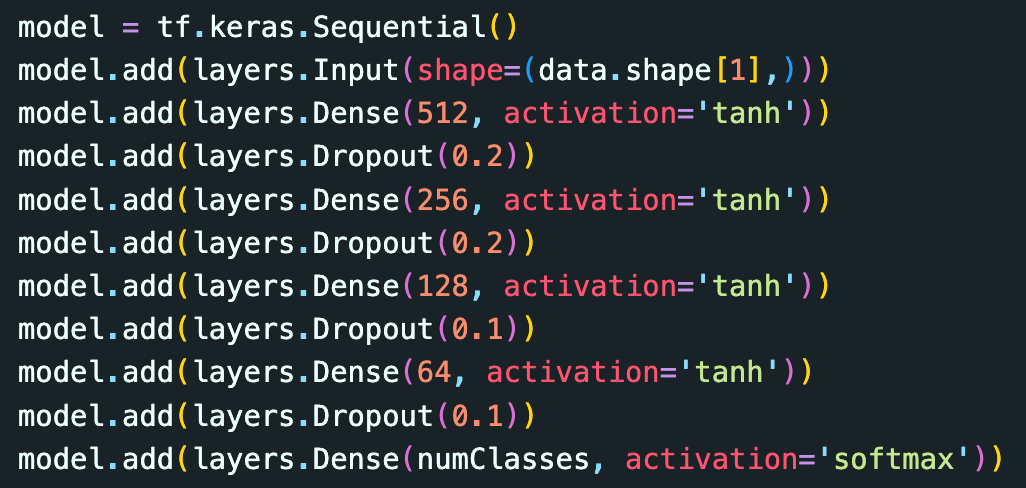
\includegraphics[width=0.7\textwidth]{figuras/ImprovedFNN.png}
    \caption{Implementación de mejoras en la red neuronal \textit{feedforward}.}
    \label{fig:dropout}
\end{figure}

\subsection{Evaluación del modelo}
Como último paso, se evaluó la habilidad del modelo para reconocer diferentes señas de la lengua de señas de Guatemala.  
Para este proceso, se utilizó una serie de videos que no se habían utilizado en el entrenamiento del modelo, los cuales se procesaron de la misma forma que los videos de entrenamiento.
La primera de estas evaluaciones se realizó con videos que contenían una sola seña, lo cual permitió evaluar la capacidad del modelo para identificar señas individuales.
Posteriormente, se evaluó el modelo con videos que contenían frases completas, lo cual permitió evaluar la capacidad del modelo para identificar frases completas.

Como métrica de evaluación, se calculó el porcentaje de videos en los cuales el modelo identificó de manera correcta la palabra correspondiente a la seña.  
Adicionalmente, se buscaron errores comunes cometidos por el modelo para que estos pudieran ser corregidos.  
Un ejemplo de esto sería si el modelo constantemente confundía una seña por otra, lo cual indicaría que el modelo necesitaba más datos correspondientes a una de esas señas o que se debía modificar el modelo.  
En este proceso de validación manual, resultó útil la codificación con la cual se identificaron los videos en la fase de preparación del conjunto de datos.

\begin{equation}
    \text{Precisión} = \frac{\text{Número de predicciones correctas}}{\text{Número total de predicciones}}
\end{equation}

Adicional a la precisión, se obtuvo la matriz de confusión, la cual permitió identificar si existían señas que eran constantemente confundidas por el modelo.
Utilizando esta información, se ajustaron los hiperparámetros del modelo y se realizaron mejoras en el conjunto de datos para corregir los errores comunes cometidos por el modelo.
La matriz de confusión también permitió calcular la sensibilidad y el puntaje F1, los cuales se utilizaron como métricas adicionales para evaluar el desempeño del modelo.

Debido a que el tiempo de procesamiento del modelo era crucial para el éxito del proyecto, se calculó la velocidad de procesamiento del modelo, en fotogramas por segundo. 
Los videos que se utilizaron en este proyecto fueron grabados a 30 fotogramas por segundo, por lo que se esperaba que el modelo pudiera procesar los videos a una velocidad similar.
Esta métrica, de fotogramas procesados por segundo, se calculó utilizando la siguiente fórmula:

\begin{equation}
    \text{Velocidad de procesamiento} = \frac{\text{Número de fotogramas procesados}}{\text{Tiempo de procesamiento}}
\end{equation}

\subsection{Evaluación del conjunto de datos}
Para evaluar el conjunto de datos, se utilizó un analizador de componentes principales (PCA) para reducir la dimensionalidad de los datos y visualizarlos en un espacio de dos dimensiones.
El PCA permitió identificar si los datos se agrupaban de forma coherente, lo cual indicaría que el modelo tendría una alta precisión al identificar las señas.
Debido a que el PCA se realizó con los datos de todos los fotogramas de video, se esperaba que los datos estuvieran algo dispersos, ya que cada fotograma de video representaba un punto en el espacio de dos dimensiones.
Lo que se buscaba con el PCA era identificar si existían señas que se agrupaban de forma similar, lo cual indicaría que el modelo tendría problemas para distinguir entre esas señas.

\begin{figure}[H]
    \centering
    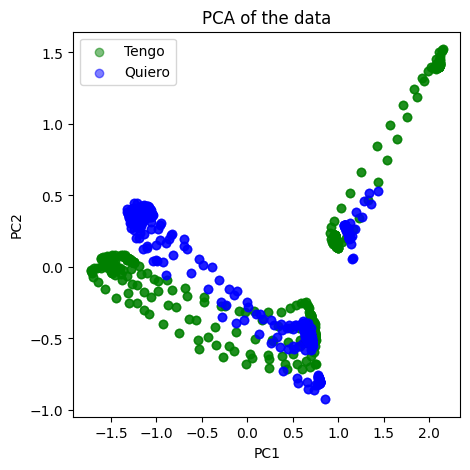
\includegraphics[width=0.7\textwidth]{figuras/ExamplePCA.png}
    \caption{Ejemplo de visualización de datos con PCA.}
    \label{fig:pca}
\end{figure}

Durante el proceso de entrenamiento del modelo, se identificaron algunas señas que eran comúnmente confundidas por el modelo. 
En estos casos, el análisis de los datos con PCA permitió identificar si existían diferencias significativas entre las señas, lo cual permitió identificar si el problema era causado por la similitud entre las señas o por la fallas en el modelo.
En la Figura \ref{fig:pca} se muestra un ejemplo de cómo se identificaron señas que no se distinguían claramente en el espacio de dos dimensiones.

Utilizando la matriz de confusión y el análisis de los datos con PCA, se buscaba identificar si los errores cometidos por el modelo eran causados por la similitud entre las señas o por fallas en el modelo.
En el caso de que los errores fueran causados por la similitud entre las señas, se esperaba que tanto la matriz de confusión como el análisis de los datos con PCA mostraran que las señas se agrupaban de forma similar.
En el caso de que los errores fueran causados por fallas en el modelo, se esperaba que la matriz de confusión mostrara que el modelo cometía errores aleatorios, mientras que el análisis de los datos con PCA mostrara que las señas se agrupaban de forma coherente.
La Figura \ref{fig:confusion_matrix} muestra un ejemplo de la matriz de confusión utilizada para evaluar el desempeño del modelo.

\begin{figure}[H]
    \centering
    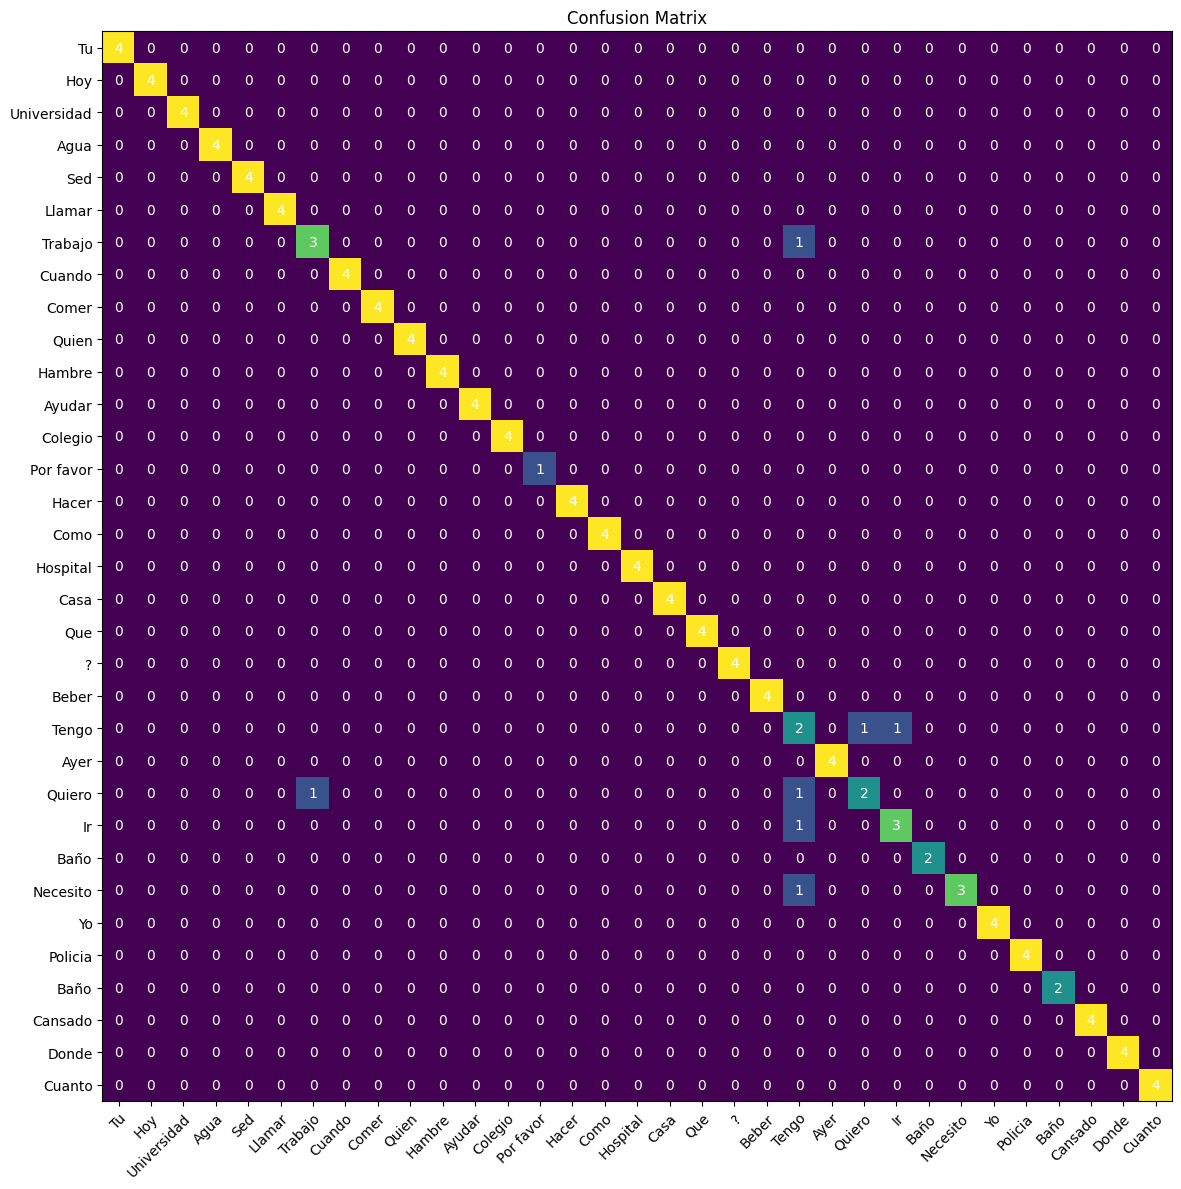
\includegraphics[width=0.7\textwidth]{figuras/ConfusionMatrixExample.png}
    \caption{Ejemplo de matriz de confusión.}
    \label{fig:confusion_matrix}
\end{figure}

\subsection{Publicación del modelo}
Una vez que el modelo fue entrenado y evaluado, se procedió a publicarlo en un servidor web para que pudiera ser utilizado por los usuarios.
Para esto, se utilizó la librería Flask de Python, la cual permitió crear una API que se comunicara con el modelo y que pudiera ser accedida por los usuarios a través de una interfaz web.
La API permitió que los usuarios enviaran videos a través de la interfaz web, los cuales se procesaban con el modelo y se devolvía la palabra correspondiente a la seña identificada.
Esto requirió de un programa adicional, diseñado para procesar los videos enviados por los usuarios y enviarlos a la API para su procesamiento.
Este programa carga el modelo entrenado, al igual que algunos parámetros adicionales, y se encarga de recibir los videos de los usuarios, procesarlos con el modelo, y devolver la palabra correspondiente a la seña identificada.
Para validar el funcionamiento de la Interfaz de Programación de Aplicaciones (API), se realizaron pruebas con videos de prueba utilizando Postman.





% Modulo de Chat
\section{Procesamiento de lenguaje natural (GPT-3.5-Turbo)} 


\subsection{Creación de conjunto de datos}

\subsubsection{Recolección de datos}

El proceso de recolección de datos consistió en buscar y seleccionar diversas frases en español que aplicaran los principios gramaticales de LENSEGUA. Para ello, se exploraron recursos en línea, como grupos en redes sociales donde usuarios sordos comparten sus pensamientos y experiencias utilizando esta gramática en sus interacciones escritas. En particular, se identificó un grupo privado en la red social Facebook llamado 'Lengua de Señas de Guatemala (LSG)'. Se envió una solicitud a los administradores del grupo para obtener acceso, y, una vez aprobada, se procedió a recopilar diversos comentarios que aplicaban esta gramática. No obstante, para proteger la privacidad de los usuarios, no se almacenó ninguna información personal, y se excluyeron comentarios que contuvieran información sensible o identificativa. Tras la recolección y almacenamiento de los datos en un archivo CSV, se generaron -de forma manual- las versiones gramaticalmente correctas en español de cada frase recopilada. En el Cuadro \ref{tab:lensegua-espanol} se presenta la estructura utilizada para almacenar la información, mostrando ejemplos de frases en LENSEGUA y sus correspondientes interpretaciones en español.

\vspace{0.5cm}
\begin{table}[H]
    \centering
    \begin{tabular}{|l|l|}
        \hline
        \textbf{LENSEGUA} & \textbf{Español} \\
        \hline
        aeropuerto dónde pregunta & ¿Dónde está el aeropuerto? \\
        \hline
        antes tu estar enojado pregunta & ¿Estabas enojado? \\
        \hline
        haber carro mucho & Hay tráfico. \\
        \hline
        pasado yo pasaporte perder & Perdí mi pasaporte. \\
        \hline
        ... & ... \\
        \hline
    \end{tabular}
    \caption{Estructura del conjunto de datos desarrollado.}
    \label{tab:lensegua-espanol}
\end{table}

Seguidamente, se establecieron contactos con organizaciones guatemaltecas que trabajan con la comunidad sorda, entre ellas la Asociación Educativa para el Sordo (ASEDES). Esta organización colaboró activamente en la generación de más ejemplos específicos que ilustraban la aplicación de la gramática de LENSEGUA en diferentes contextos, desde situaciones cotidianas hasta emergencias. Ellos se centraron en utilizar un vocabulario que tuviera equivalentes directos en LENSEGUA, ya que no todas las palabras en español tienen una traducción literal en lengua de señas. Además, colaboraron con la creación de las versiones gramaticalmente correctas en español para cada una de estas frases, manteniendo la misma estructura descrita anteriormente.

\vspace{0.5cm}
\begin{figure}[H]
  \centering
  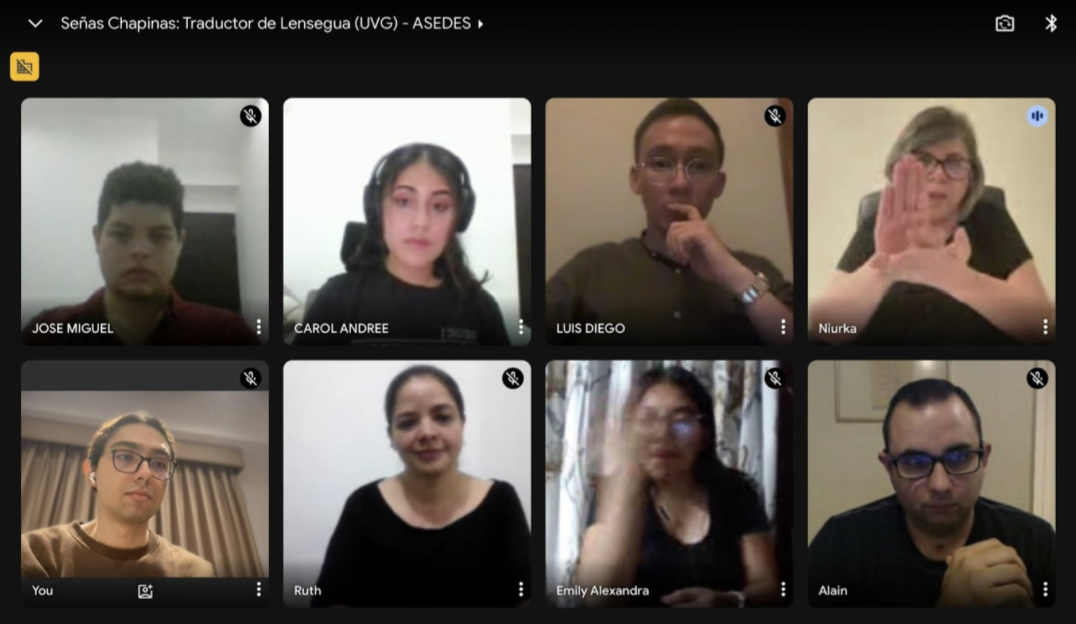
\includegraphics[width=0.9\linewidth]{figuras/ASEDES.png}
  \caption{Reunión de equipo de trabajo con ASEDES.}
  \label{fig:ASEDES}
\end{figure}

Durante esta etapa, se optó por recibir un curso virtual sobre la gramática de LENSEGUA ofrecido por la organización Sordos Latinos Guatemala. Este curso proporcionó una comprensión detallada de las reglas y estructuras gramaticales específicas de LENSEGUA, lo que permitió generar ejemplos adicionales -propios- con mayor precisión. Además, la capacitación también facilitó la validación de los textos anteriormente obtenidos, asegurando que el contenido estuviera alineado con las normas gramaticales de LENSEGUA.

Por último, se tomó como referencia en el trabajo de Fan \textit{et al.} (2023) \cite{thirtyeight} y se procedió a utilizar la plataforma de Claude.ai para generar más datos. Más específicamente, se le proporcionó a esta herramienta de generación de texto (basada en inteligencia artificial) el archivo CSV anteriormente desarrollado y se solicitó que generara entradas adicionales para ampliar el \textit{dataset}. Este proceso tuvo como objetivo incrementar tanto la cantidad como la diversidad de los ejemplos disponibles en el \textit{dataset}. Posteriormente, se revisaron las frases generadas para asegurar que cumplieran con las normas gramaticales de LENSEGUA y se verificó que no hubiera duplicados en el contenido.

Cabe destacar que no se utilizó ChatGPT para generar los datos adicionales, ya que no se considera óptimo \textit{fine-tunear} un modelo con salidas generadas por la misma herramienta. Este acercamiento no aportaría nueva información y resultaría en redundancia en el aprendizaje \cite{thirtyeight}. Por ello, se eligió Claude.ai, una plataforma independiente, para garantizar que los datos fueran verdaderamente nuevos, permitiendo así que el proceso de \textit{fine-tuning} en GPT-3.5-Turbo se basara en entradas totalmente nuevas y variadas.


\subsubsection{Data augmentation}

Una vez generados los datos iniciales, se procedió a dividir el conjunto de datos en dos subconjuntos: un 80\% se destinó al entrenamiento y un 20\% a la evaluación. Esta división fue necesaria para evaluar el rendimiento del modelo de manera efectiva y garantizar que el modelo final no se sobreajustara a los datos de entrenamiento.

Después de esta separación, se desarrolló un programa en Python con el propósito de realizar \textit{data augmentation} en el conjunto de entrenamiento. Es decir, ampliar el \textit{dataset} existente mediante la generación de nuevas frases. El enfoque consistió en crear variaciones de las frases originales mediante la sustitución de palabras por otras similares, manteniendo la coherencia contextual. Por ejemplo, una oración como ‘papá cirujano ser’ podría transformarse en ‘abuelo doctor ser’ y ‘tío odontólogo ser’, entre otras (ver la Figura \ref{fig:RECUR}).

\begin{figure}[H]
  \centering
  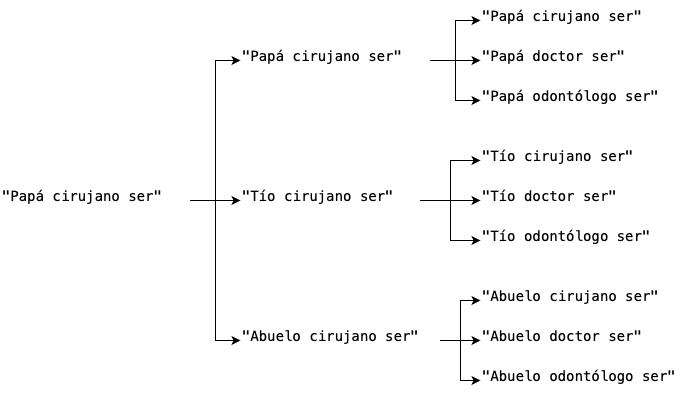
\includegraphics[width=0.9\linewidth]{figuras/RECUR.png}
  \caption{Generación recursiva de nuevas frases.}
  \label{fig:RECUR}
\end{figure}

Para ello, se definió un conjunto de listas que agrupaban palabras intercambiables, como profesiones, lugares, objetos, entre otros. El programa analizaba cada oración del conjunto de entrenamiento y, al identificar términos presentes en estas listas, generaba todas las posibles combinaciones de oraciones mediante sustituciones recursivas. De esta manera, si una oración contenía varias palabras intercambiables, se creaban múltiples variantes de la misma, ampliando significativamente el \textit{dataset} de entrenamiento.

Es importante mencionar que el sistema de \textit{data augmentation} también modificaba las interpretaciones teóricas definidas en el \textit{dataset}. Esto aseguraba que cada nueva frase en LENSEGUA tuviera su correspondiente versión en español, aumentando así la cantidad de datos disponibles para el \textit{fine-tuning} del modelo GPT-3.5-Turbo.


\subsubsection{Preparación del conjunto de datos}

Con el \textit{dataset} de entrenamiento ampliado y el conjunto de evaluación definido, se procedió a preparar los datos utilizando Python. Este proceso incluyó la corrección automatizada de mayúsculas y la adición de signos de puntuación, entre otros ajustes. Además, se organizaron los datos en un formato compatible con OpenAI, utilizando un formato JSON con la siguiente estructura:

\vspace{0.5cm}
\begin{lstlisting}
'messages': [
    {'role': 'system', 'content': DEFAULT_SYSTEM_PROMPT},
    {'role': 'user', 'content': question + ' ->'},
    {'role': 'assistant', 'content': answer},
]
\end{lstlisting}
\vspace{0.3cm}

En esta estructura, el \textit{DEFAULT SYSTEM PROMPT} constituye el mensaje inicial que establece el contexto y las directrices fundamentales para el comportamiento del modelo. El campo \textit{question} contiene la frase que aplica la gramática de LENSEGUA, mientras que el campo \textit{answer} proporciona la interpretación gramaticalmente correcta en español. 

Al finalizar con la preparación, los datos procesados se guardaron en archivos JSONL, asegurando así su disponibilidad para el siguiente paso en el proceso de \textit{fine-tuning} del modelo. 



\subsection{Fine-tuning}


\subsubsection{Identificación de parámetros óptimos}

Para asegurar un rendimiento óptimo del modelo \textit{fine-tuneado} GPT-3.5-Turbo, se realizaron pruebas preliminares con una porción del conjunto de datos (se excluyeron las frases generadas mediante \textit{data augmentation}). Estas pruebas permitieron experimentar con distintas configuraciones para identificar los parámetros más adecuados. Al emplear un subconjunto del \textit{dataset}, se optimizó el proceso sin incurrir en los altos costos asociados a múltiples entrenamientos completos, logrando además acelerar el proceso ajuste fino.

Los parámetros ajustados incluyeron:

\begin{itemize}
    \item \textbf{Epochs}: Número de veces que el modelo recorre el conjunto de datos de entrenamiento completo. Ajustar este parámetro fue clave para evitar tanto el subentrenamiento como el sobreentrenamiento.
    
    \item \textbf{Batch size}: Cantidad de muestras procesadas antes de actualizar los parámetros del modelo. Valores pequeños favorecen la generalización, mientras que valores grandes aceleran el entrenamiento.
    
    \item \textbf{Learning Rate Multiplier}: Controla la magnitud de los ajustes que realiza el modelo en función de los errores durante el entrenamiento. Un ajuste adecuado de este parámetro fue crucial para asegurar la convergencia del modelo.
\end{itemize}


\subsubsection{Fine-tuning del modelo GPT-3.5-Turbo}

Una vez identificados los parámetros óptimos, se realizó el \textit{fine-tuning} del modelo GPT-3.5-Turbo en la plataforma de OpenAI. Para ello, se creó una nueva tarea de \textit{fine-tuning} y se seleccionó el modelo base correspondiente. Luego, se cargaron los archivos JSONL generados previamente. El archivo de entrenamiento incluía 4,192 entradas, combinando frases originales y aquellas generadas mediante \textit{data augmentation}. Por su parte, el archivo de validación contenía 200 entradas para evaluar el rendimiento del modelo durante el ajuste. Finalmente, se configuraron los parámetros y se inició el proceso de \textit{fine-tuning}.

Durante el proceso de ajuste, se monitoreó la pérdida de entrenamiento y validación para verificar que el modelo no presentara \textit{overfitting}. El \textit{overfitting} ocurre cuando un modelo aprende demasiado bien los datos de entrenamiento, afectando así su capacidad de generalización. 


\subsubsection{Evaluación del modelo GPT-3.5-Turbo fine-tuneado}

\paragraph{Distancia de Levenshtein}

Tras completar el proceso de \textit{fine-tuning}, se procedió a evaluar el desempeño del modelo en la generación de interpretaciones utilizando la distancia de Levenshtein. Esta métrica mide el número mínimo de operaciones necesarias (inserciones, eliminaciones o sustituciones) para transformar una cadena de texto en otra \cite{thirtynine}. Se consideró que esta métrica era particularmente adecuada para este contexto, ya que el objetivo era que el modelo generara interpretaciones sin introducir variaciones significativas en el vocabulario ni en la estructura de las frases. 

Para llevar a cabo esta evaluación, se desarrolló un programa en Python que permitió al modelo \textit{fine-tuneado} generar interpretaciones para cada frase del conjunto de validación, utilizando un \textit{prompt} básico que definía el rol del sistema como intérprete de LENSEGUA. A partir de esto, se compararon las interpretaciones generadas con las interpretaciones teóricas predefinidas y se calculó la distancia de Levenshtein para cada par. Finalmente, se promediaron las 200 distancias obtenidas, lo que permitió determinar un valor representativo del desempeño del modelo.

Con el fin de establecer una línea de comparación, se repitió el análisis con el modelo GPT-3.5-Turbo estándar, utilizando las mismas 200 frases y el mismo \textit{prompt}. En este caso, el modelo que presentó la menor distancia promedio fue considerado el más efectivo para la tarea de interpretación.

\paragraph{Local Interpretable Model-agnostic Explanations (LIME)}

La técnica de \textit{Local Interpretable Model-agnostic Explanations} (LIME) se utilizó para obtener una comprensión más profunda del impacto del \textit{fine-tuning}. LIME permitió identificar, para frases individuales, qué palabras tuvieron mayor influencia en la interpretación generada por cada modelo. De este modo, se buscaba determinar cómo los elementos característicos de LENSEGUA influían en las respuestas de cada modelo, y si el modelo \textit{fine-tuneado} mostraba una recepción más favorable hacia estos elementos en comparación con el modelo estándar.

El análisis se realizó utilizando Python y la librería LIME. A este programa se le proporcionaron tres frases de prueba, entre ellas “pasado yo ir no”. Cada frase fue sometida a un proceso de perturbación, que consistió en generar cien variaciones mediante la eliminación aleatoria de palabras. Estas frases modificadas se enviaron a ambos modelos (el modelo \textit{fine-tuneado} y el modelo GPT-3.5-Turbo estándar) para que generaran sus interpretaciones utilizando el \textit{prompt} básico previamente mencionado.

El Cuadro \ref{tab:LIME} presenta un ejemplo del resultado este proceso. En la primera fila, se muestra la frase seleccionada y su correspondiente interpretación teórica, que en este caso es “No fui”. Seguidamente, se detallan algunas perturbaciones generadas a partir de la frase original, junto con las interpretaciones producidas por el modelo \textit{fine-tuneado}. Es importante mencionar que este mismo procedimiento se realizó utilizando el modelo GPT-3.5-Turbo estándar, generando así un conjunto comparable de interpretaciones para cada perturbación.

Para comparar las interpretaciones generadas con respecto a las interpretaciones teóricas, se utilizó la distancia de Levenshtein normalizada. Este valor, que oscila entre 0 y 1, permite determinar la similitud de entre dos frases. Un valor de 1 indica que las frases son idénticas, mientras que valores más bajos reflejan mayores diferencias.

\vspace{0.5cm}
\begin{table}[h!]
\centering
\begin{tabular}{|l|l|c|}
\hline
        \multicolumn{3}{|l|}{\textbf{Frase en LENSEGUA:} pasado yo ir no} \\ \hline
        \multicolumn{3}{|l|}{\textbf{Interpretación teórica:} No fui.} \\ \hline \hline
        \parbox{3cm}{\centering \textbf{Frase /} \\ \textbf{Perturbación}} & \textbf{Interpretación} & \parbox{4cm}{\centering \textbf{Distancia de} \\ \textbf{Levenshtein (norm.)}} \\ \hline
        pasado yo ir no        & No fui.                           & 1.0            \\ \hline
        yo                     & Yo.                           & 0.2857         \\ \hline
        pasado yo no           & No fui.                           & 1.0            \\ \hline
        pasado                 & En el pasado.                     & 0.1538         \\ \hline
        ...                     & ...                               & ...         \\ \hline
\end{tabular}
\caption{Ejemplos de perturbaciones interpretadas por el modelo \textit{fine-tuneado} junto con sus distancias de Lenveshtein normalizadas correspondientes.}
\label{tab:LIME}
\end{table}

A partir de los resultados obtenidos mediante las perturbaciones y sus correspondientes distancias de Levenshtein normalizadas, LIME permitió cuantificar la influencia de cada palabra en las interpretaciones generadas tanto por el modelo estándar como el \textit{fine-tuneado}. Un valor positivo indicaba que una palabra ayudaba al modelo a generar interpretaciones más cercanas a la teórica, mientras que un valor bajo o negativo sugería que su presencia confundía al modelo, resultando en respuestas más distantes de lo esperado. 



\subsection{Prompt engineering}

Durante la evaluación del modelo \textit{fine-tuneado}, se identificaron varios aspectos que afectaron negativamente la calidad de las interpretaciones generadas. En particular, se observaron dificultades en el manejo de expresiones temporales, lo que llevaba a errores de interpretación y redundancias en las respuestas. Para abordar estas limitaciones, se implementó una fase de \textit{prompt engineering} con el objetivo de mejorar la coherencia y precisión de las interpretaciones.

Se desarrollaron nuevas versiones del \textit{prompt} de manera iterativa, incorporando instrucciones más precisas y delimitadores específicos. Cada nueva versión se diseñó a partir de la evaluación de la versión anterior, lo que permitió un refinamiento continuo de las instrucciones. Las modificaciones incluyeron la adición de reglas explícitas para el procesamiento de expresiones características de LENSEGUA, así como ejemplos contextuales. Estos cambios se orientaron a potenciar la capacidad del modelo para interpretar correctamente el contexto y a minimizar las ambigüedades en las respuestas.

Para evaluar cada \textit{prompt}, se utilizó el programa de Python previamente desarrollado en la fase de \textit{fine-tuning}. Este programa permitió generar interpretaciones para cada frase del conjunto de validación, utilizando las distintas versiones de los \textit{prompts}. A partir de estas interpretaciones, se calculó la distancia de Levenshtein promedio para medir la similitud entre las respuestas generadas y las interpretaciones teóricas predefinidas. De esta manera, se logró determinar una distancia promedio asociada a cada \textit{prompt}, lo que proporcionó una medida cuantitativa del rendimiento de cada versión. Cabe destacar que este proceso de evaluación se realizó tanto con el modelo \textit{fine-tuneado} como con el modelo GPT-3.5-Turbo estándar, lo que facilitó la comparación del impacto de cada \textit{prompt} en ambos modelos.

    
\subsection{Implementación y evaluación del sistema}

Uno de los objetivos principales de este proyecto fue que miembros de la comunidad sorda evaluaran la coherencia y precisión de las interpretaciones generadas por el modelo \textit{fine-tuneado}. Para ello, se desarrolló una plataforma web que le permitió a usuarios interactuar directamente con el sistema y evaluar su rendimiento en tiempo real. Además, se diseñó una encuesta dirigida a intérpretes, estudiantes y usuarios familiarizados con LENSEGUA, con el propósito de calificar el desempeño del modelo \textit{fine-tuneado} en comparación con la versión estándar de GPT-3.5-Turbo. Esta combinación de interacción directa a través de la plataforma web y una evaluación estructurada proporcionó una visión completa sobre la efectividad de las interpretaciones generadas, ofreciendo una base sólida para analizar el rendimiento del sistema.


\subsubsection{Desarrollo de plataforma web}

Para facilitar la interacción con el modelo \textit{fine-tuneado}, se desarrolló una plataforma web local (no accesible desde el internet) para que permitía a los usuarios probar el sistema de manera controlada. Esta aplicación se estructuró en dos componentes principales: el \textit{backend}, responsable del procesamiento de las solicitudes a través de Python y Flask, y el \textit{frontend}, encargado de la visualización de los resultados en tiempo real.

El \textit{backend} del sistema estableció una conexión con el API de OpenAI, lo que permitió la interacción directa tanto con el modelo \textit{fine-tuneado} como con otros modelos de OpenAI. Además, se encargó de gestionar las solicitudes de los usuarios: cuando un usuario introducía una frase, el \textit{backend} enviaba la solicitud a la API, procesaba la respuesta generada por el modelo y devolvía la interpretación correspondiente. Se implementó también un sistema de almacenamiento de historial de solicitudes, que permitió a los usuarios visualizar el registro completo de sus consultas.

El \textit{frontend} se desarrolló utilizando HTML y CSS, lo que permitió crear una interfaz de usuario intuitiva y eficiente. La página web adoptó un formato similar al de un \textit{chat}, facilitando a los usuarios la entrada de frases y la recepción de respuestas en tiempo real. Además, se incluyó la opción de seleccionar entre el modelo \textit{fine-tuneado} y el modelo GPT-3.5-Turbo estándar. La interfaz fue optimizada para dispositivos de escritorio, garantizando así una experiencia clara y amigable.


\subsubsection{Desarrollo de encuesta}

Para evaluar la coherencia de las frases generadas por el modelo \textit{fine-tuneado}, se creó una encuesta mediante Google Forms. La encuesta comenzaba con un consentimiento informado que detallaba el propósito del estudio y el proceso de evaluación, asegurando que los participantes comprendieran plenamente la metodología antes de iniciar. 

La encuesta se organizó en secciones, cada una enfocada en evaluar una frase específica mediante tres preguntas. Las dos primeras preguntas solicitaban a los participantes que calificaran, en una escala del 1 al 5 (donde 1 representaba baja coherencia y 5 alta coherencia), las interpretaciones generadas tanto por el modelo estándar GPT-3.5-Turbo como por el modelo \textit{fine-tuneado}. La tercera pregunta requería una comparación directa entre ambas interpretaciones, pidiendo a los participantes que seleccionaran la que consideraban más coherente o adecuada para la frase en cuestión.

Además, la encuesta incluía una sección adicional dedicada a evaluar los diferentes \textit{prompts} desarrollados. En esta sección, los participantes debían seleccionar, entre varias opciones, la interpretación que encontraban más clara y comprensible. Todas estas interpretaciones fueron generadas por el modelo \textit{fine-tuneado}, pero utilizando diferentes \textit{prompts}. Esta metodología permitió no solo evaluar la coherencia general del modelo \textit{fine-tuneado}, sino también validar cuál \textit{prompt} resultaba más efectivo para la generación de interpretaciones precisas.

Es fundamental mencionar que la encuesta se limitó a participantes que eran personas sordas, familiares de personas sordas, estudiantes de LENSEGUA o intérpretes. Esta selección garantizó que las evaluaciones provinieran de individuos con un conocimiento relevante sobre la lengua, lo que contribuyó a la validez de los resultados obtenidos.


\subsubsection{Pruebas con usuarios}

En la etapa final de evaluación del modelo, se organizó una reunión presencial con la asociación guatemalteca de sordos En-Señas. La sesión inició con una presentación detallada del modelo \textit{fine-tuneado}, en la que se explicó su propósito y funcionamiento. Además, los participantes, en su mayoría personas sordas y un intérprete, pudieron observar el sistema en acción y hacer preguntas sobre su desarrollo. Posteriormente, se les pidió completar la encuesta previamente descrita, donde evaluaron la coherencia de las interpretaciones generadas por el modelo. Esta interacción directa fue clave para recopilar comentarios y sugerencias en tiempo real, lo que contribuyó a una evaluación más completa del sistema. Las respuestas de estos participantes, como se detallará más adelante, permitieron confirmar la efectividad del modelo desarrollado, resaltando su utilidad en la interpretación de frases que aplican la gramática de LENSEGUA.

Para ampliar el alcance de la evaluación, la encuesta se compartió también con otras organizaciones y clubes de LENSEGUA. Esto permitió obtener un conjunto más amplio de respuestas, enriqueciendo así el análisis de la coherencia y utilidad del modelo \textit{fine-tuneado}.













































% Modulo de LLaMA
\section{Procesamiento de lenguaje natural (LLaMA)} 


\subsection{Creación de conjunto de datos}

\subsubsection{Recolección de datos}

El conjunto de datos utilizado para este módulo mantuvo la misma estructura que el empleado durante el entrenamiento del modelo GPT-3.5-Turbo. Sin embargo, se optó por crear datos completamente diferentes para este proceso. 

Cada entrada en el conjunto de datos consistía en una frase escrita que utilizaba la gramática específica de LENSEGUA y su correspondiente versión gramaticalmente correcta en español. Este enfoque permitió representar de manera adecuada las características únicas de LENSEGUA y su relación con el español escrito. Los datos fueron diseñados por expertos con conocimiento avanzado en la gramática de LENSEGUA, asegurando la coherencia y precisión en cada ejemplo.

Los 560 pares de frases se guardaron en un archivo CSV, lo que facilitó su organización y procesamiento en las etapas posteriores del proyecto.


\subsubsection{Preparación del conjunto de datos}

Una vez recopilados los datos, estos se procesaron para cumplir con el formato requerido por el modelo seleccionado, Alpaca. Este modelo, desarrollado por la Universidad de Stanford, es una versión ajustada de LLaMA. Su formato compatible, estructurado en JSON, se compone de tres campos principales:

\vspace{0.5cm}
\begin{lstlisting}
{
    "instruction": "",
    "input": [LENSEGUA],
    "output": [INTERPRETACION]
}
\end{lstlisting}
\vspace{0.3cm}

El campo \textit{instruction} especifica la tarea que se desea realizar con el modelo, es decir, la instrucción que la LLM debe completar. El \textit{input} es un campo que proporciona contexto adicional. Este contexto puede ser información o detalles relevantes que ayudan al modelo a interpretar correctamente la instrucción, como referencias gramaticales o aclaraciones específicas. Por otro lado, el campo \textit{output} contiene la respuesta esperada según la instrucción proporcionada. 

Para organizar adecuadamente los datos, se dividieron en tres archivos JSON, siguiendo la estructura mencionada de \textit{instruction}, \textit{input} y \textit{output}. Más específicamente, 70\% de los datos se destinaron al entrenamiento del modelo, 15\% para validación y 15\% para prueba. Esta división equilibrada permitió un ajuste efectivo del modelo y una evaluación precisa de su rendimiento en las distintas etapas del proceso.







\subsection{Configuración inicial}

Para trabajar con LLaMA, se empleó la biblioteca \textit{Transformers} de Hugging Face, la cual ofrece herramientas eficientes para cargar, entrenar y realizar \textit{fine-tuning} en modelos de lenguaje. En particular, se utilizó la versión LLaMA 3.0 con 8 mil millones de parámetros (\textit{8B}) debido a las limitaciones de recursos disponibles.

\subsubsection{Entorno de desarrollo}

La biblioteca \textit{Transformers} ofrece compatibilidad con Unidades de Procesamiento Gráfico (GPUs) mediante la utilización de la Arquitectura Unificada de Dispositivos de Cómputo (CUDA), desarrollada por NVIDIA. CUDA es una plataforma que maximiza el poder computacional de las GPUs, permitiendo realizar procesamiento en paralelo de manera eficiente. Como se muestra en la Figura \ref{fig:cpu_gpu}, las GPUs son fundamentales para manejar las exigencias de los LLMs, ya que permiten el procesamiento paralelo de millones de hilos de ejecución. Esto optimiza tanto el entrenamiento como la ejecución de los modelos, especialmente en tareas que requieren cálculos intensivos \cite{nvidia2024cuda}.

\vspace{0.5cm}
\begin{figure}[h] \begin{center} 
\includegraphics[height=5.5 cm]{plantilla/GPU.png} \caption{Comparación entre CPU y GPU en el procesamiento paralelo.} \label{fig:cpu_gpu} \end{center} \end{figure}

Dado que el uso de GPUs dedicadas puede ser costoso y requiere infraestructura especializada, se optó por utilizar Google Colab como entorno de desarrollo. Este servicio proporciona acceso gratuito a GPUs en la nube, lo cual permite ejecutar proyectos complejos sin depender de recursos locales. Además, su entorno basado en Python facilita la integración con bibliotecas como \textit{Transformers}, simplificando tanto la configuración como la experimentación en tareas de procesamiento de lenguaje natural.



\subsubsection{Cuantización y Low-Rank Adaptation (LoRA)}

Una vez configurado el ambiente en Google Colab, se procedió a cargar el modelo LLaMA 3.0 utilizando Python y la biblioteca \textit{Transformers}. Para optimizar su uso y permitir su entrenamiento en un entorno con limitaciones de \textit{hardware}, se aplicaron dos técnicas clave: cuantización y \textit{Low-Rank Adaptation} (LoRA).

En primer lugar, el proceso de cuantización consistió en reducir la precisión de los pesos del modelo de 32 bits a 8 bits. Esta reducción permitió disminuir significativamente los requerimientos de memoria y el tiempo necesario para los cálculos de los pesos, haciendo el modelo más eficiente en términos computacionales. Aunque este enfoque sacrifica ligeramente la precisión del modelo, se logró un balance adecuado entre eficiencia y calidad, lo que lo hizo apto para el \textit{fine-tuning} en un entorno con recursos limitados como Google Colab.

Dado que los LLMs contienen una gran cantidad de parámetros, el entrenamiento completo de estos modelos resulta costoso y poco práctico, ya que requiere actualizar todos los pesos de manera intensiva en recursos. \textit{Low-Rank Adaptation} (LoRA) resuelve esta problemática al aplicar matrices de bajo rango en ciertas capas de un modelo pre-entrenado, como se ilustra en la Figura \ref{fig:LORA}. Esta técnica es particularmente efectiva para ajustar LLMs a nuevas tareas sin necesidad de realizar un entrenamiento completo y sin perder el conocimiento preexistente. De esta manera, LoRA mejora la capacidad de adaptación del modelo a nuevas situaciones, manteniendo la eficiencia computacional \cite{Jawade2023}.

\begin{figure}[h] \begin{center} 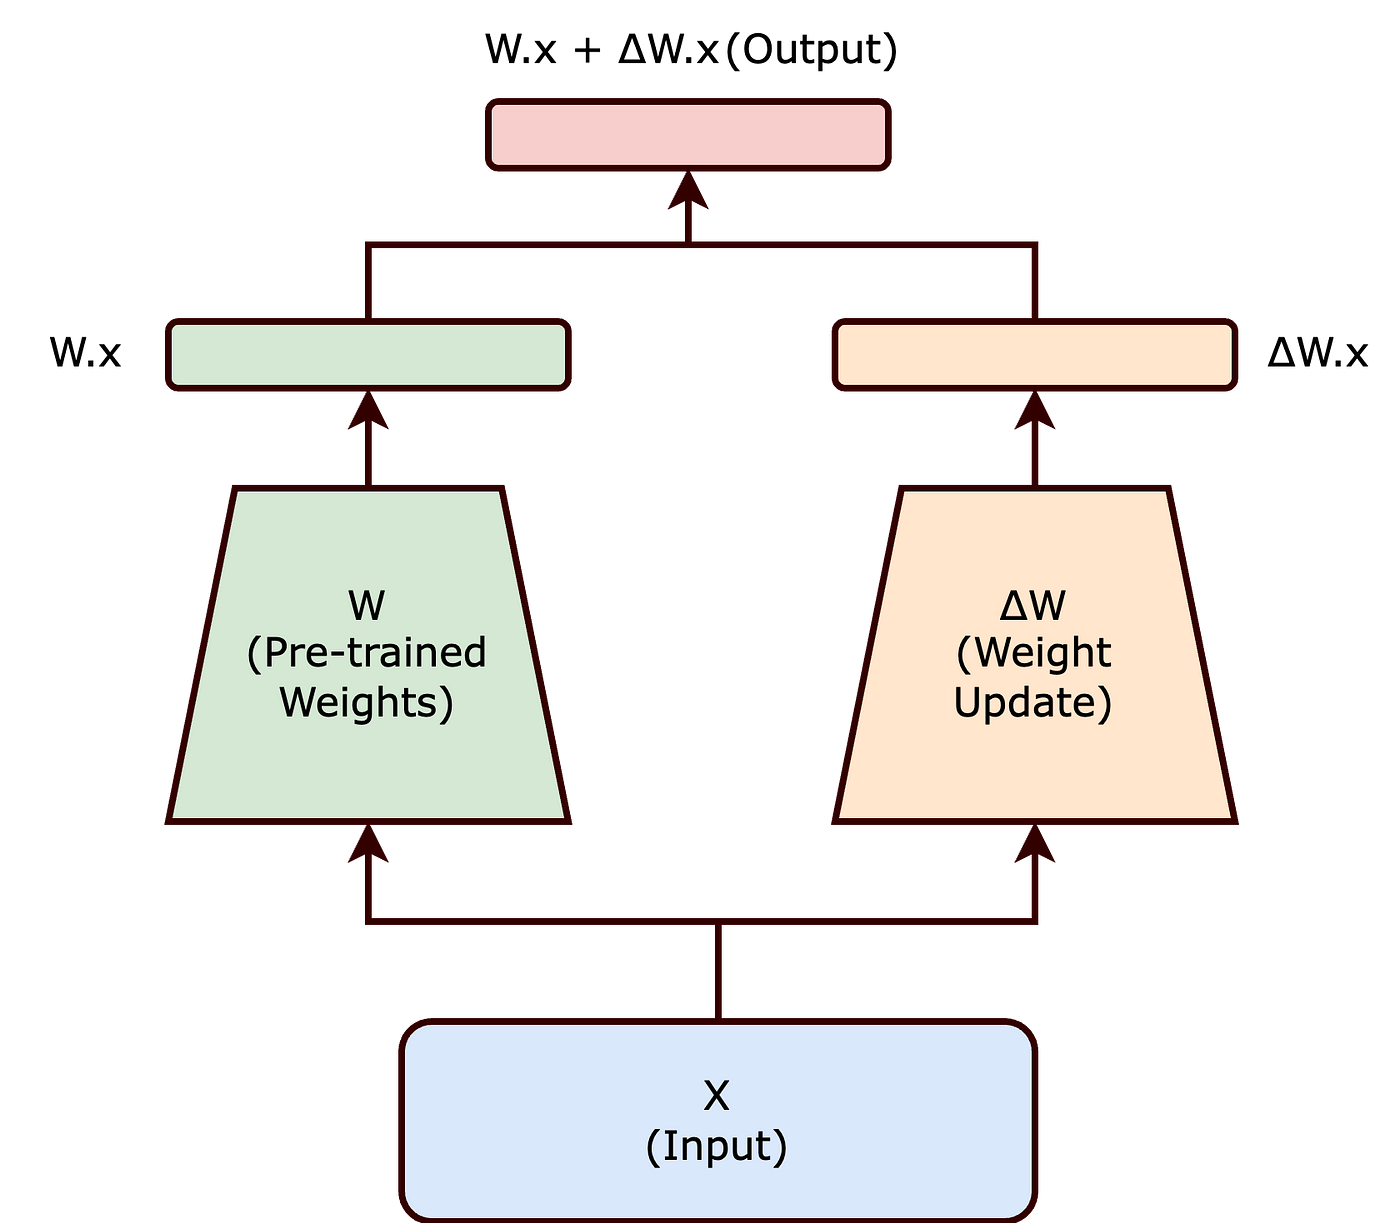
\includegraphics[height=5.5 cm]{plantilla/Lora.png} 
\caption{Diagrama de entrenamiento con LoRA.}
\label{fig:LORA} \end{center} \end{figure}

Los dos parámetros clave en LoRA son el rango y el alpha, los cuales controlan la capacidad del modelo para adaptarse a nuevas tareas sin comprometer demasiado la eficiencia o el rendimiento.

\begin{itemize}
    \item \textbf{Rango:} Define la dimensión del espacio de bajo rango utilizado para la adaptación. Un rango mayor permite una adaptación más precisa, pero requiere más recursos computacionales. Un rango demasiado grande puede generar \textit{overfitting}, mientras que un rango muy pequeño puede no ser suficiente para capturar las características relevantes de los datos.
    \item \textbf{Alpha:} Es el factor de escala que controla la magnitud de la adaptación. Un alpha alto incrementa la magnitud de los ajustes, lo que puede llevar a \textit{overfitting}. Un alpha bajo puede no ser suficiente para adaptar el modelo correctamente a la tarea.
\end{itemize}





\subsection{Fine-tuning}

\subsubsection{Identificación de parámetros óptimos}

Para la identificación de los parámetros óptimos para el proceso de \textit{fine-tuning} del modelo LLaMA, se llevaron a cabo múltiples pruebas utilizando un subconjunto reducido del conjunto de entrenamiento. El objetivo principal fue encontrar las configuraciones que produjeran los mejores resultados en términos de la métrica BLEU, así como en pérdida de validación.

Durante las primeras tres pruebas, se utilizó un entrenador genérico, lo cual permitió una mayor flexibilidad en el proceso de entrenamiento. Este enfoque permitió al modelo decidir libremente si entrenar de manera supervisada o no supervisada.

En la primera prueba, se entrenó el modelo sin ningún ajuste específico, con el objetivo de verificar su funcionamiento básico. En la segunda prueba, se aplicó la técnica de \textit{early stopping} para evitar sobreentrenar el modelo y mejorar la generalización, reduciendo el número de \textit{batches} de entrenamiento. 

Es importante mencionar que en todas las pruebas se utilizó LoRA. Sin embargo, durante el tercer experimento, se implementó una configuración estándar de LoRA, ajustando los parámetros de rango y alpha a valores de 8 y 16, respectivamente, siguiendo las recomendaciones de un estudio de traducción bilingüe \cite{weller2022pretrained}. Estos valores fueron seleccionados para asegurar una adaptación eficiente y controlada sin comprometer la capacidad computacional. En esta tercera prueba también se hizo uso de la técnica de \textit{early stopping}.

En la cuarta prueba, se tomó la decisión de reducir la flexibilidad del modelo al pasar a un enfoque más estricto de \textit{fine-tuning} supervisado. Es decir, se forzó al modelo a entrenar de manera supervisada, eliminando la capacidad de decidir si entrenar de forma supervisada o no. A pesar de este cambio, se mantuvo el estándar de LoRA con los parámetros de rango y alpha en 8 y 16, respectivamente. Además, se continuó utilizando la técnica de \textit{early stopping} para evitar el sobreentrenamiento y mejorar la generalización del modelo.


\subsubsection{Fine-tuning del modelo LLaMA (versión 1)}

La combinación de parámetros utilizada en la cuarta prueba, que incluyó un enfoque más estricto de \textit{fine-tuning} supervisado junto con los valores de LoRA para el rango y alpha de 8 y 16 respectivamente, presentó los mejores resultados en términos de la métrica BLEU y la pérdida de validación. Debido a estos resultados prometedores, se decidió repetir el proceso de \textit{fine-tuning} utilizando esta configuración, pero con el conjunto de datos completo. Durante este proceso, se monitoreó cuidadosamente la pérdida de entrenamiento y validación para asegurar que el modelo no presentara \textit{overfitting}. 

Una vez completado el \textit{fine-tuning}, se procedió a evaluar el rendimiento del modelo. Para ello, se le pidió al modelo que generara interpretaciones para todo el conjunto de prueba, calculando la métrica BLEU para cada par de interpretación generada y esperada, lo que permitió obtener un valor promedio representativo de su precisión. Adicionalmente, se utilizó la técnica LIME para analizar el impacto del \textit{fine-tuning} en las interpretaciones del modelo. Este análisis permitió identificar la relevancia asignada por el modelo a palabras específicas, proporcionando información valiosa sobre cómo el ajuste afectó su comportamiento. 

Posteriormente, se solicitó la colaboración de una intérprete experta en LENSEGUA para realizar un análisis cualitativo de las interpretaciones generadas. Este enfoque permitió evaluar la calidad de las interpretaciones desde una perspectiva lingüística y práctica, validando si cumplían con los estándares de calidad esperados. Aunque los resultados obtenidos fueron aceptables, se consideró que las métricas, como BLEU, podrían mejorar si el \textit{fine-tuning} se realizaba de manera más exhaustiva. Por lo tanto, se decidió repetir la tarea de \textit{fine-tuning} utilizando un conjunto de datos más grande, pero manteniendo la configuración óptima identificada.

\subsubsection{Fine-tuning del modelo LLaMA (versión 2)}

En esta segunda versión, se decidió utilizar el conjunto de datos desarrollado específicamente para el \textit{fine-tuning} del modelo GPT-3.5-Turbo. Este conjunto estaba compuesto por dos archivos: el archivo de entrenamiento, con 4,192 entradas, y el archivo de validación, con 200 entradas diseñadas para evaluar el rendimiento del modelo durante el ajuste. 

Nuevamente, se mantuvo la configuración óptima identificada en las pruebas previas, incluyendo los valores de LoRA para rango y alpha, así como el uso de la técnica de \textit{early stopping}, con el objetivo de evitar el \textit{overfitting} y mejorar la generalización. Sin embargo, el uso de este conjunto de datos, más extenso y diverso, permitió al modelo aprender patrones más complejos y relevantes para las tareas de interpretación de LENSEGUA.

El proceso de \textit{fine-tuning} incluyó un monitoreo constante de las métricas de rendimiento, como la pérdida de entrenamiento y validación. Además, se evaluó el modelo utilizando el conjunto de validación, generando interpretaciones que se compararon con las esperadas mediante dos métricas principales: BLEU, para medir la precisión en las interpretaciones, y la distancia de Levenshtein, para analizar las diferencias estructurales entre las interpretaciones generadas y las esperadas. A partir de estas comparaciones, se calcularon valores promedio que proporcionaron una evaluación detallada del desempeño del modelo.

Finalmente, para profundizar en el análisis, se utilizó LIME para evaluar el impacto del \textit{fine-tuning} en las interpretaciones del modelo, identificando la relevancia asignada a palabras específicas en las entradas. 


\subsection{Comparación de modelos fine-tuneados (GPT-3.5-Turbo y LLaMA)}

Tras completar el último proceso de \textit{fine-tuning} del modelo LLaMA, se realizó una comparación con el modelo GPT-3.5-Turbo, también ajustado mediante \textit{fine-tuning}. Dado que ambos modelos fueron entrenados con el mismo conjunto de datos, fue posible llevar a cabo una evaluación consistente de su desempeño. La comparación se llevó a cabo utilizando dos enfoques principales: la distancia promedio de Levenshtein y los análisis realizados mediante LIME, enfocándose en identificar las diferencias clave en la calidad y relevancia de las interpretaciones producidas por ambos modelos.










































% MODULO AQUITECTURA DE RED ==================================

\section{Infraestructura de red}

\subsection{Levantamiento de un sistema operativo y configuración de VPN}

Para garantizar un ambiente de trabajo seguro y eficiente, se ha implementado Ubuntu 22.08 como sistema operativo en un servidor Dell R740. Se elimino el controlador RAID para liberar un disco duro de 1.92T, adecuándolo para las necesidades del proyecto. Además, se configuró una VPN utilizando OpenVPN, lo cual permite un acceso directo y seguro a los servidores. La configuración de la VPN se complementó con ajustes en los firewalls institucionales otorgados por la universidad, facilitando el acceso remoto y el manejo del servidor desde múltiples dispositivos sin comprometer la seguridad. Esta configuración permite una administración centralizada y segura del servidor, asegurando que solo usuarios autorizados puedan acceder a los recursos críticos del sistema. 

Como se puede observar en la Figura \ref{fig:LevantadoOpenVPN}, la máquina virtual fue levantada correctamente. Además, en la Figura \ref{fig:ConexionSSH} se muestra la conexión generada con la VPN mediante SSH.

\begin{figure}[H]
    \centering
    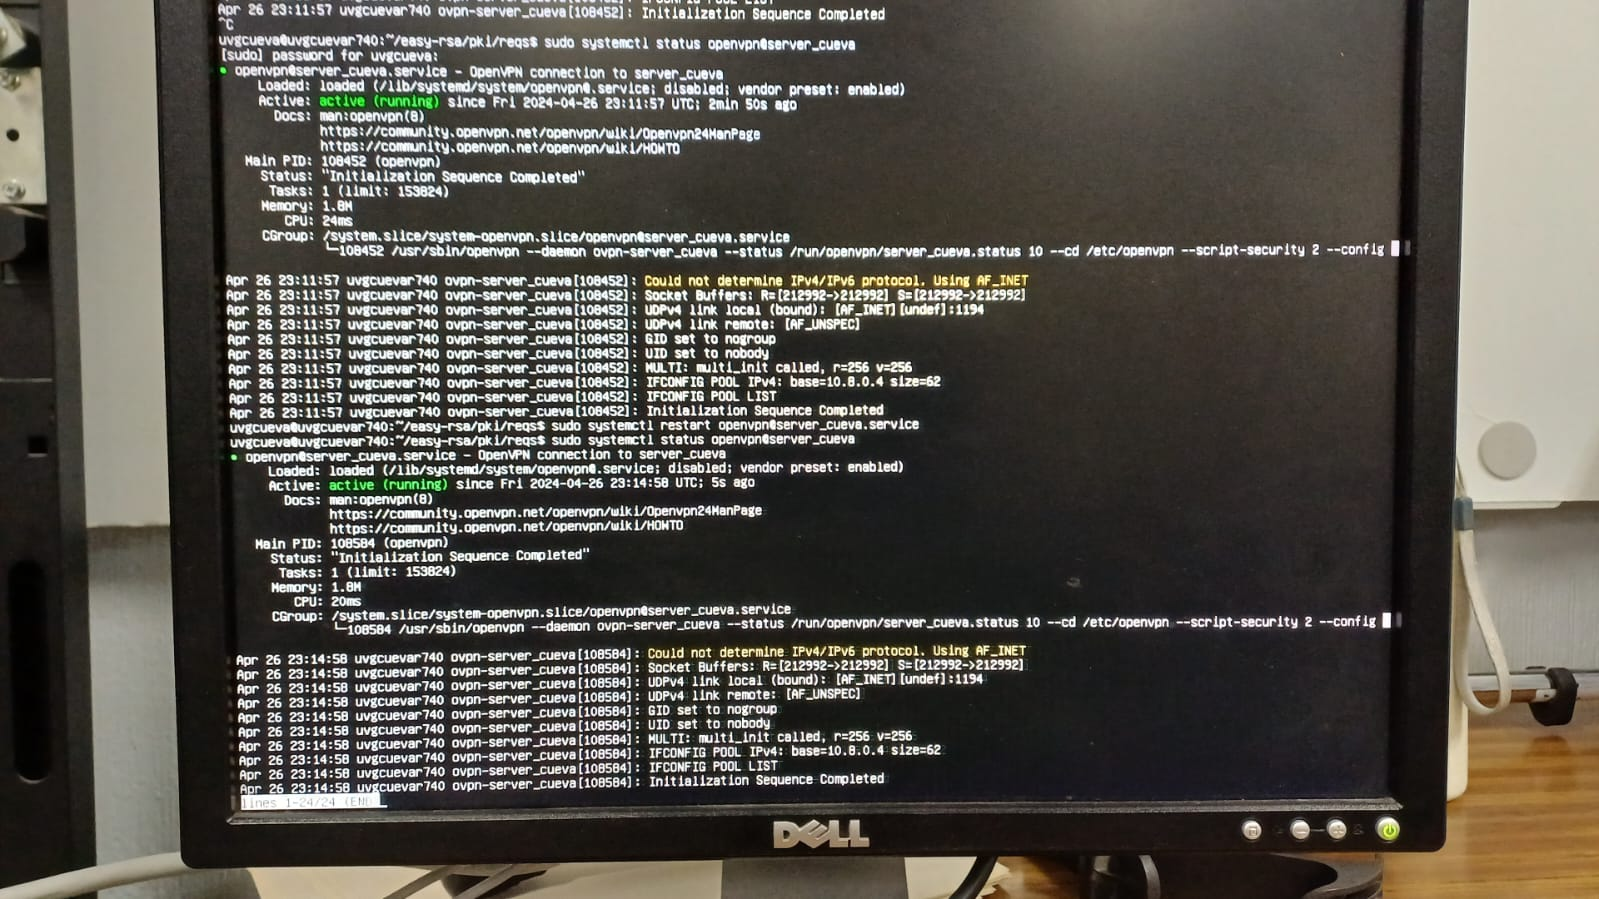
\includegraphics[width=0.7\textwidth]{figuras/LevantadoOpenVPN.png}
    \caption{LevantadoOpenVPN.}
    \label{fig:LevantadoOpenVPN}
\end{figure}


\begin{figure}[H]
    \centering
    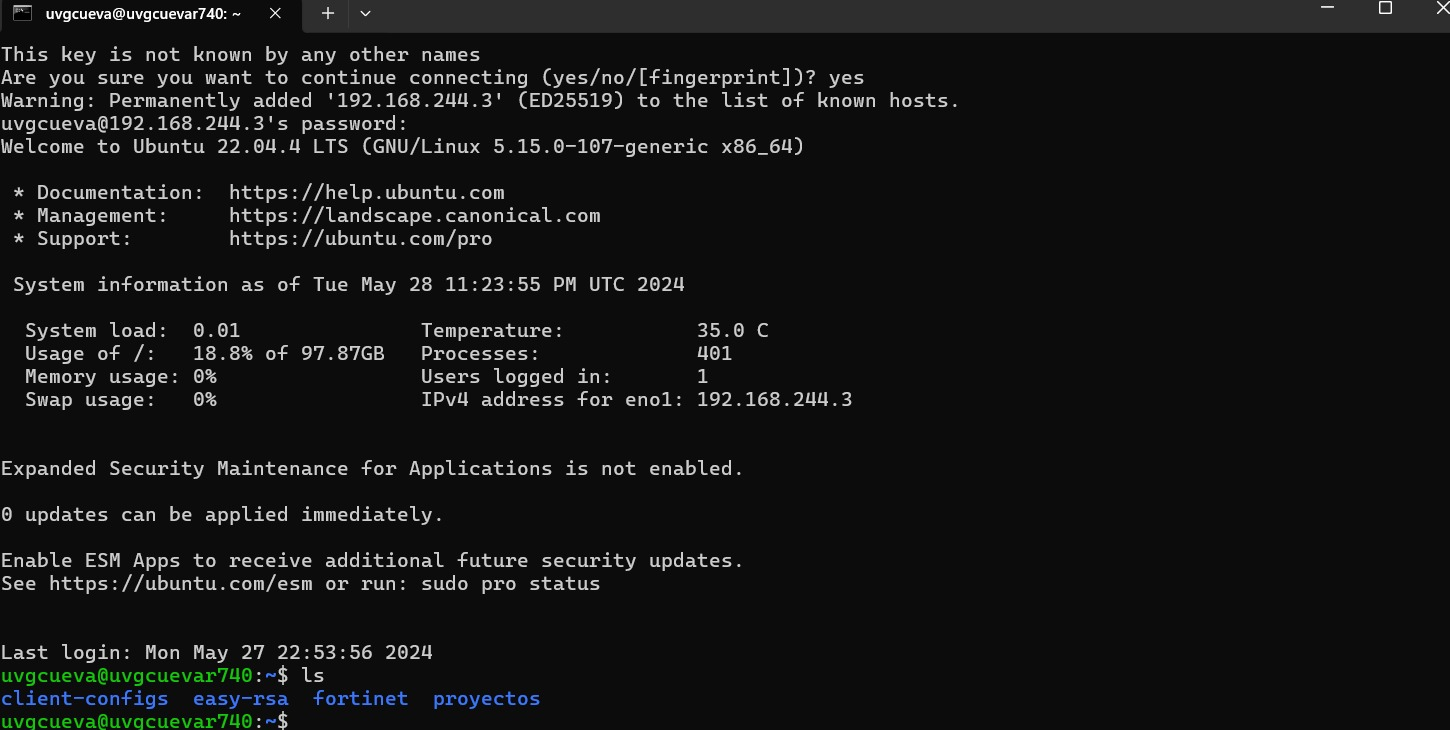
\includegraphics[width=0.7\textwidth]{figuras/ConexionSSH.png}
    \caption{ConexionSSH.}
    \label{fig:ConexionSSH}
\end{figure}

El proceso requirió conectarse a través de la infraestructura de red de la universidad y la VLAN específica donde se encontraba el rack y el servidor. Para lograr esto, se utilizó FortiClient VPN, que proporcionó una conexión segura y cifrada directamente a la VLAN donde se encontraba el servidor. Para acceder a la VPN, se necesitó un archivo de configuración .ovpn que se utilizó con OpenVPN. Una vez conectados a la VPN, se pudo acceder al servidor de manera segura mediante SSH. Esto se realizó abriendo una terminal y utilizando el comando `ssh uvgcueva@192.168.244.3` con las credenciales correspondientes. Este método aseguró que la administración remota de las máquinas virtuales se realizara de manera eficiente y segura, permitiendo a los usuarios realizar tareas administrativas y de mantenimiento sin estar físicamente presentes en el sitio.

\subsection{Desarrollo de la arquitectura de base de datos}

Se seleccionó PostgreSQL para gestionar la base de datos relacional del proyecto debido a su robustez y eficacia en el manejo de grandes volúmenes de datos, incluyendo datos de usuarios, videos y otros tipos de información. PostgreSQL ofreció avanzadas características de seguridad que fueron esenciales para proteger los datos contra accesos no autorizados. Su arquitectura permitió realizar operaciones complejas de base de datos de manera eficiente, asegurando la integridad y la privacidad de los datos gestionados. En la arquitectura se hizo especial hincapié en la importancia de diseñar con flexibilidad, utilizando estándares que permitieran la interacción entre diferentes sistemas y tecnologías.

Para implementar PostgreSQL en el proyecto de forma efectiva y segura, se siguió una metodología estructurada que abarcó desde la planificación inicial hasta la integración con otros sistemas. Comenzamos evaluando los requisitos de hardware y software para seleccionar la versión óptima de PostgreSQL y preparar el entorno del sistema operativo. Una vez instalado PostgreSQL, se procedió a configurar los parámetros de rendimiento y seguridad, como la memoria, conexiones permitidas y configuraciones de cifrado, además de establecer un protocolo regular de mantenimiento que incluyó actualizaciones y parches.

La seguridad fue una prioridad, implementando roles y permisos detallados para controlar el acceso a los datos y asegurar todas las comunicaciones mediante SSL/TLS. Paralelamente, se desarrollaron y configuraron procesos de ETL para automatizar la extracción, transformación y carga de datos, asegurando la integridad y utilidad de la información gestionada. Además, se diseñaron y desarrollaron APIs que permitieron una interacción segura y eficiente con otras aplicaciones, implementando mecanismos robustos de autenticación y autorización.

Finalmente, se establecieron sistemas de monitoreo para supervisar constantemente el rendimiento y la seguridad de la base de datos y las APIs, permitiendo ajustes continuos para optimizar la configuración según las necesidades cambiantes del proyecto. Este enfoque metodológico aseguró no solo la implementación técnica efectiva de PostgreSQL, sino también el mantenimiento de un sistema seguro, eficiente y adaptable a largo plazo.


% Cuadros de la base de datos
% ---------------------------

% Tabla: user
\begin{table}[H]
\centering
\begin{tabularx}{\textwidth}{|l|l|l|X|}
\hline
\textbf{Nombre del campo} & \textbf{Tipo de dato} & \textbf{Restricciones} & \textbf{Descripción} \\ \hline
id                       & Integer               & Primary Key            & Identificador único del usuario. \\ \hline
mail                     & String(120)           & Unique, Not Null       & Correo electrónico del usuario. \\ \hline
password                 & String(120)           & Not Null               & Contraseña del usuario. \\ \hline
streak                   & Integer               & Default = 0            & Puntuación o racha del usuario. \\ \hline
quetzalito               & String                & Nullable               & Color de la imagen de perfil. \\ \hline
confirmed                & Boolean               & Default=False          & Indica si el usuario ha confirmado su cuenta. \\ \hline
\texttt{last\_streak\_update} & DateTime            & Default=datetime.utcnow & Indica la última hora que se agregó un streak. \\ \hline
\end{tabularx}
\caption{Tabla: user}
\end{table}

% Tabla: video
\begin{table}[H]
\centering
\begin{tabularx}{\textwidth}{|l|l|l|X|}
\hline
\textbf{Nombre del campo} & \textbf{Tipo de dato} & \textbf{Restricciones} & \textbf{Descripción} \\ \hline
id                       & Integer               & Primary Key            & Identificador único del video. \\ \hline
id\_user                 & Integer               & ForeignKey(user.id), Not Null & Referencia al usuario que subió el video. \\ \hline
traduction\_esp          & String(255)           & Nullable                & Traducción del video al español. \\ \hline
sentence\_lensegua       & String(255)           & Not Null                & Oración en lengua de señas guatemalteca. \\ \hline
video                    & String(255)           & Not Null                & Ruta del archivo de video. \\ \hline
prev\_image              & String(255)           & Nullable                & Imagen previa del video. \\ \hline
is\_favorite             & Boolean               & Default=False           & Indica si el video es favorito del usuario. \\ \hline
\end{tabularx}
\caption{Tabla: video}
\end{table}

% Tabla: traducción
\begin{table}[H]
\centering
\begin{tabularx}{\textwidth}{|l|l|l|X|}
\hline
\textbf{Nombre del campo} & \textbf{Tipo de dato} & \textbf{Restricciones} & \textbf{Descripción} \\ \hline
id                       & Integer               & Primary Key            & Identificador único de la traducción. \\ \hline
id\_user                 & Integer               & ForeignKey(user.id), Not Null & Referencia al usuario que hizo la traducción. \\ \hline
sentence\_lensegua       & String(255)           & Not Null                & Oración en lengua de señas guatemalteca. \\ \hline
traduction\_esp          & String(255)           & Nullable                & Traducción al español. \\ \hline
is\_favorite             & Boolean               & Default=False           & Indica si la traducción es favorita. \\ \hline
\end{tabularx}
\caption{Tabla: traducción}
\end{table}

% Tabla: dictionary
\begin{table}[H]
\centering
\begin{tabularx}{\textwidth}{|l|l|l|X|}
\hline
\textbf{Nombre del campo} & \textbf{Tipo de dato} & \textbf{Restricciones} & \textbf{Descripción} \\ \hline
id                       & Integer               & Primary Key            & Identificador único del diccionario. \\ \hline
id\_user                 & Integer               & ForeignKey(user.id), Not Null & Referencia al usuario. \\ \hline
id\_word                 & String(255)           & Not Null                & Palabra o identificador del término en el diccionario. \\ \hline
\end{tabularx}
\caption{Tabla: dictionary}
\end{table}

El diagrama de entidad-relación presentado en la Figura \ref{fig:entidad_relacion} muestra la estructura y las relaciones entre las tablas diseñadas para el proyecto. 

En este diagrama se observan las entidades principales del sistema: \texttt{user}, \texttt{video}, \texttt{traducción} y \texttt{dictionary}. Cada una de estas entidades incluye atributos que definen su propósito dentro del sistema. Por ejemplo, la tabla \texttt{user} almacena información esencial del usuario como su correo, contraseña y estado de confirmación, mientras que la tabla \texttt{video} registra información de los videos asociados a los usuarios, incluyendo traducciones y metadatos adicionales.

Las relaciones entre las entidades destacan cómo interactúan entre sí. Por ejemplo, la tabla \texttt{video} está vinculada a la tabla \texttt{user} mediante una relación de uno a muchos (\texttt{1:N}), lo que indica que cada usuario puede tener múltiples videos asociados. Asimismo, la tabla \texttt{traducción} permite almacenar traducciones específicas realizadas por los usuarios, vinculándose también a través de una relación de \texttt{1:N} con \texttt{user}.

Este diseño garantizó la flexibilidad y escalabilidad del sistema, permitiendo el manejo eficiente de los datos necesarios para cumplir con los objetivos del proyecto.

\begin{figure}[H]
    \centering
    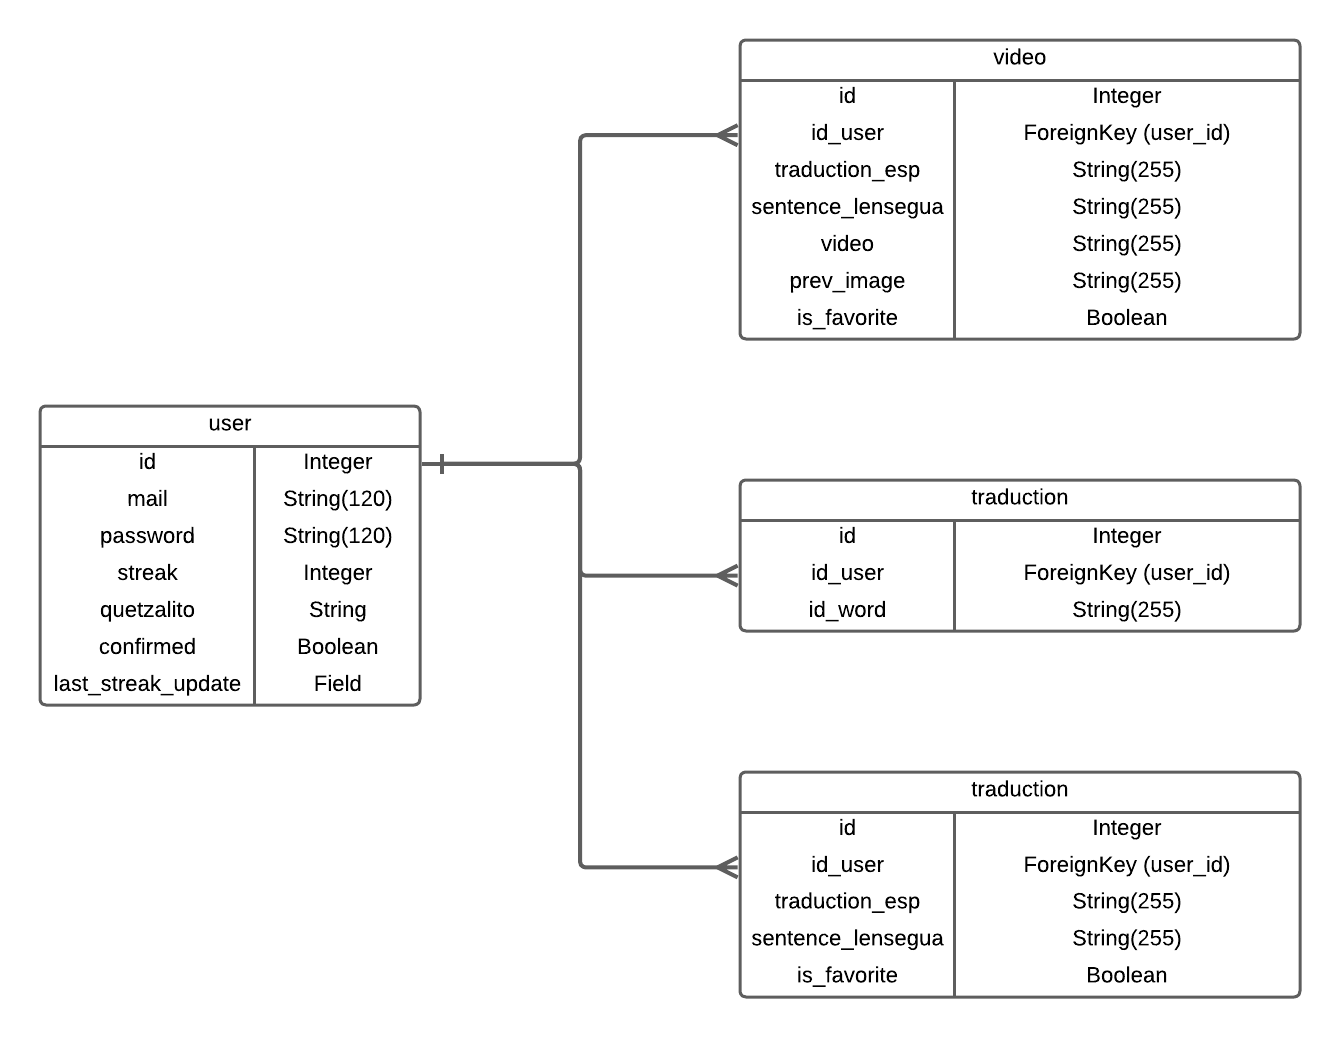
\includegraphics[width=0.5\textwidth]{figuras/entidad_relacion.png}
    \caption{Diagrama entidad relación.}
    \label{fig:entidad_relacion}
\end{figure}

% Fin de cuadros de la base de datos
% ---------------------------

\subsection{Implementacion de APIs}

Para facilitar las consultas y las inserciones de datos, se utilizó Flask como framework principal debido a su ligereza y capacidad para manejar peticiones de manera eficiente. Este módulo API permitió un manejo flexible de diferentes formatos de datos, incluyendo videos y texto. La estructura del módulo estuvo diseñada para optimizar el rendimiento del sistema, minimizando el uso de recursos y maximizando la velocidad de respuesta, lo que fue crucial para procesar y responder a las interacciones de los usuarios en tiempo real.

% Definir colores personalizados para las filas
\definecolor{lightgreen}{RGB}{199,233,192}
\definecolor{lightblue}{RGB}{180,220,240}
\definecolor{lightred}{RGB}{252,205,205}

% Tabla para las APIS
% -------------------

% Tabla de user_routes
\begin{table}[H]
\centering
\begin{tabularx}{\textwidth}{|l|l|l|X|}
\hline
\textbf{Nombre} & \textbf{TIPO} & \textbf{Entrada} & \textbf{Salida} \\ \hline
login & POST & email, password & id\_user \\ \hline
signup & POST & email, password, quetzalito & id\_user \\ \hline
forgot\_password & POST & email & 200-OK \\ \hline
change\_password & POST & id\_user, new\_password & id\_user, 200-OK \\ \hline
\end{tabularx}
\caption{Resumen de Rutas de API: \texttt{user\_routes}}
\label{tab:user_routes}
\end{table}

% Tabla de video_routes
\renewcommand{\arraystretch}{1.3} % Aumenta la altura de las filas
\begin{table}[H]
\centering
\begin{tabularx}{\textwidth}{|l|l|X|X|}
\hline
\textbf{Nombre} & \textbf{TIPO} & \textbf{Entrada} & \textbf{Salida} \\ \hline
send\_video & POST & id\_user, video & id\_video, traduction\_lensegua, traduction\_esp \\ \hline
report\_video & POST & id\_user, id\_video, report\_message, report\_img (png) & 200-OK \\ \hline
fav\_video & POST & id\_user, id\_video, prev\_video (png) & 200-OK \\ \hline
remove\_video & DELETE & id\_video & 200-OK \\ \hline
remove\_fav\_video & POST & id\_user, id\_video & 200-OK \\ \hline
download\_video & POST & route\_video & ruta\_video \\ \hline
download\_images & POST & route\_image & ruta\_image \\ \hline
\end{tabularx}
\caption{Resumen de Rutas de API: \texttt{video\_routes}}
\label{tab:video_routes}
\end{table}

% Tabla de traduction_routes
\begin{table}[H]
\centering
\begin{tabularx}{\textwidth}{|l|l|l|X|}
\hline
\textbf{Nombre} & \textbf{TIPO} & \textbf{Entrada} & \textbf{Salida} \\ \hline
send\_traduction & POST & id\_user, sentence\_lensegua & id\_sentence, traduction\_esp \\ \hline
fav\_traduction & POST & id\_user, id\_sentence & 200-OK \\ \hline
remove\_traduction & DELETE & id\_sentence & 200-OK \\ \hline
remove\_fav\_traduction & POST & id\_user, id\_sentence & 200-OK \\ \hline
\end{tabularx}
\caption{Resumen de Rutas de API: traduction\_routes}
\label{tab:traduction_routes}
\end{table}

% Tabla de dictionary_routes
\begin{table}[H]
\centering
\begin{tabularx}{\textwidth}{|l|l|l|X|}
\hline
\textbf{Nombre} & \textbf{TIPO} & \textbf{Entrada} & \textbf{Salida} \\ \hline
add\_dictionary & POST & id\_user, id\_word & 200-OK \\ \hline
remove\_dictionary & DELETE & id\_user, id\_word & 200-OK \\ \hline
get\_dictionary & POST & id\_user & palabras (json) \\ \hline
\end{tabularx}
\caption{Resumen de Rutas de API: \texttt{dictionary\_routes}}
\label{tab:dictionary_routes}
\end{table}

% Tabla de profile_routes
\begin{table}[H]
\centering
\begin{tabularx}{\textwidth}{|l|l|l|X|}
\hline
\textbf{Nombre} & \textbf{TIPO} & \textbf{Entrada} & \textbf{Salida} \\ \hline
get\_user\_info & POST & id\_user & email, streak, quetzalito, videos\_fav (json), traductions\_fav (json) \\ \hline
get\_video & POST & id\_user, id\_video & video (mp4) \\ \hline
get\_image & POST & id\_user, id\_video & image (png) \\ \hline
delete\_user & DELETE & id\_user & 200-OK \\ \hline
add\_streak & POST & id\_user & 200-OK \\ \hline
remove\_streak & POST & id\_user & 200-OK \\ \hline
\end{tabularx}
\caption{Resumen de Rutas de API: \texttt{profile\_routes}}
\label{tab:profile_routes}
\end{table}

% Tabla de mail_routes
\begin{table}[H]
\centering
\begin{tabularx}{\textwidth}{|l|l|l|X|}
\hline
\textbf{Nombre} & \textbf{TIPO} & \textbf{Entrada} & \textbf{Salida} \\ \hline
confirm & POST & email & 200-OK \\ \hline
\end{tabularx}
\caption{Resumen de Rutas de API: \texttt{mail\_routes}}
\label{tab:mail_routes}
\end{table}


% Fin de las tablas para APIS
% ---------------------------
% AQUI: meter la imagen de resultadosDeLlamarUsandoSQLAlchemy

\subsubsection{Flujo de trabajo para sistema de APIs}

La infraestructura del sistema sigue un flujo bien definido en el manejo de solicitudes y respuestas, diseñado para garantizar un equilibrio entre eficiencia y robustez.

\begin{enumerate}
    \item \textbf{Cliente envía una solicitud:} 
    El punto de partida se da cuando un cliente realiza una solicitud HTTP al servidor, por ejemplo, \texttt{mi-ip:4242/example}. Este podría ser un navegador web, una aplicación móvil, o cualquier sistema que consuma las APIs que estamos desarrollando. En este primer punto, la solicitud se envía al servidor en la ruta definida.

    \item \textbf{Nginx recibe la solicitud:} 
    Nginx actúa como la primera línea de defensa y como un proxy inverso. Es el encargado de recibir todas las solicitudes entrantes y decidir cómo deben ser manejadas. Nginx no solo se encarga de redirigir las solicitudes, sino que también es clave en el manejo de conexiones concurrentes, balanceo de carga y la administración de recursos estáticos si es necesario. Gracias a Nginx, el sistema puede gestionar eficientemente un alto volumen de solicitudes simultáneas, \textit{distribuyéndolas} entre los diferentes trabajadores de Gunicorn.

    \item \textbf{Nginx reenvía la solicitud a Gunicorn:} 
    Una vez que Nginx recibe la solicitud, la reenvía a Gunicorn utilizando un socket Unix o TCP, según la configuración definida. Gunicorn es un servidor de aplicaciones WSGI diseñado específicamente para ejecutar aplicaciones Flask en entornos de producción. En este paso, Gunicorn toma la solicitud y la pasa al núcleo de la aplicación Flask.

    \item \textbf{Gunicorn procesa la solicitud:} 
    Al recibir la solicitud de Nginx, Gunicorn la envía a la aplicación Flask, encargada de manejar la lógica de negocio asociada a cada \textit{endpoint}. Por ejemplo, si la solicitud se realizó a la ruta \texttt{/example}, Flask ejecutará la función asociada a esa ruta. Esta función puede incluir lógica para consultar una base de datos, realizar cálculos, o incluso comunicarse con otros servicios.

    \item \textbf{Flask genera y envía la respuesta:} 
    Una vez que Flask ha procesado la solicitud, genera una respuesta adecuada. Esta respuesta puede estar en formato JSON, HTML, o cualquier otro formato según lo requerido por el cliente. Posteriormente, Flask devuelve la respuesta a Gunicorn, que se encargará de llevarla al siguiente paso en el flujo.

    \item \textbf{Gunicorn reenvía la respuesta a Nginx:} 
    Al recibir la respuesta de Flask, Gunicorn la reenvía a Nginx, que tiene la responsabilidad de empaquetarla y prepararla para ser entregada de vuelta al cliente.

    \item \textbf{Nginx devuelve la respuesta al cliente:} 
    Finalmente, Nginx envía la respuesta al cliente que hizo la solicitud. El cliente recibe la respuesta HTTP, que puede ser procesada y presentada de acuerdo a sus necesidades. Este paso cierra el ciclo de la solicitud, asegurando que el sistema haya gestionado de manera eficiente tanto la entrada como la salida de información.
\end{enumerate}


\subsubsection{Diagrama de flujo de la arquitectura de solicitudes}

En esta sección se presenta el diagrama de flujo de la arquitectura del proyecto (Figura \ref{fig:diagrama_flujo}), el cual ilustra cómo se gestionan las solicitudes en el sistema. Nuestra estructura sigue el principio de "dividir y conquistar", separando las múltiples solicitudes en secciones que tienen objetivos específicos y bien definidos. 

Las solicitudes se agrupan en diferentes módulos, cada uno manejado por un archivo dedicado:
\begin{itemize}
    \item \textbf{profile\_routes.py:} Gestiona operaciones relacionadas con la información del perfil del usuario, como obtener datos personales, videos y traducciones favoritas, y la gestión de la racha (\textit{streak}).
    \item \textbf{user\_routes.py:} Maneja operaciones de autenticación y registro, como iniciar sesión, registrarse, y cambiar contraseñas.
    \item \textbf{video\_routes.py:} Se ocupa de la carga, gestión y eliminación de videos, así como de marcar o desmarcar favoritos y manejar imágenes de previsualización.
    \item \textbf{traduction\_routes.py:} Administra las traducciones de frases en Lensegua al español, permitiendo marcar traducciones como favoritas o eliminarlas.
    \item \textbf{dictionary\_routes.py:} Permite agregar, eliminar y consultar palabras en el diccionario de favoritos del usuario.
    \item \textbf{mail\_routes.py:} Facilita el envío de correos electrónicos, como en el caso de restablecimiento de contraseñas.
\end{itemize}

Todos estos módulos giran en torno al uso del archivo \textbf{models.py}, el cual actúa como el eje central del sistema. Este archivo define las entidades y modelos utilizados para interactuar con la base de datos, permitiendo que todas las secciones puedan acceder y realizar operaciones en ella de manera eficiente y centralizada.

Esta división modular asegura una arquitectura organizada, fácil de mantener y escalable, donde cada módulo se encarga de tareas específicas, mientras que el modelo central proporciona una única fuente de verdad para la interacción con los datos.

\begin{figure}[H]
    \centering
    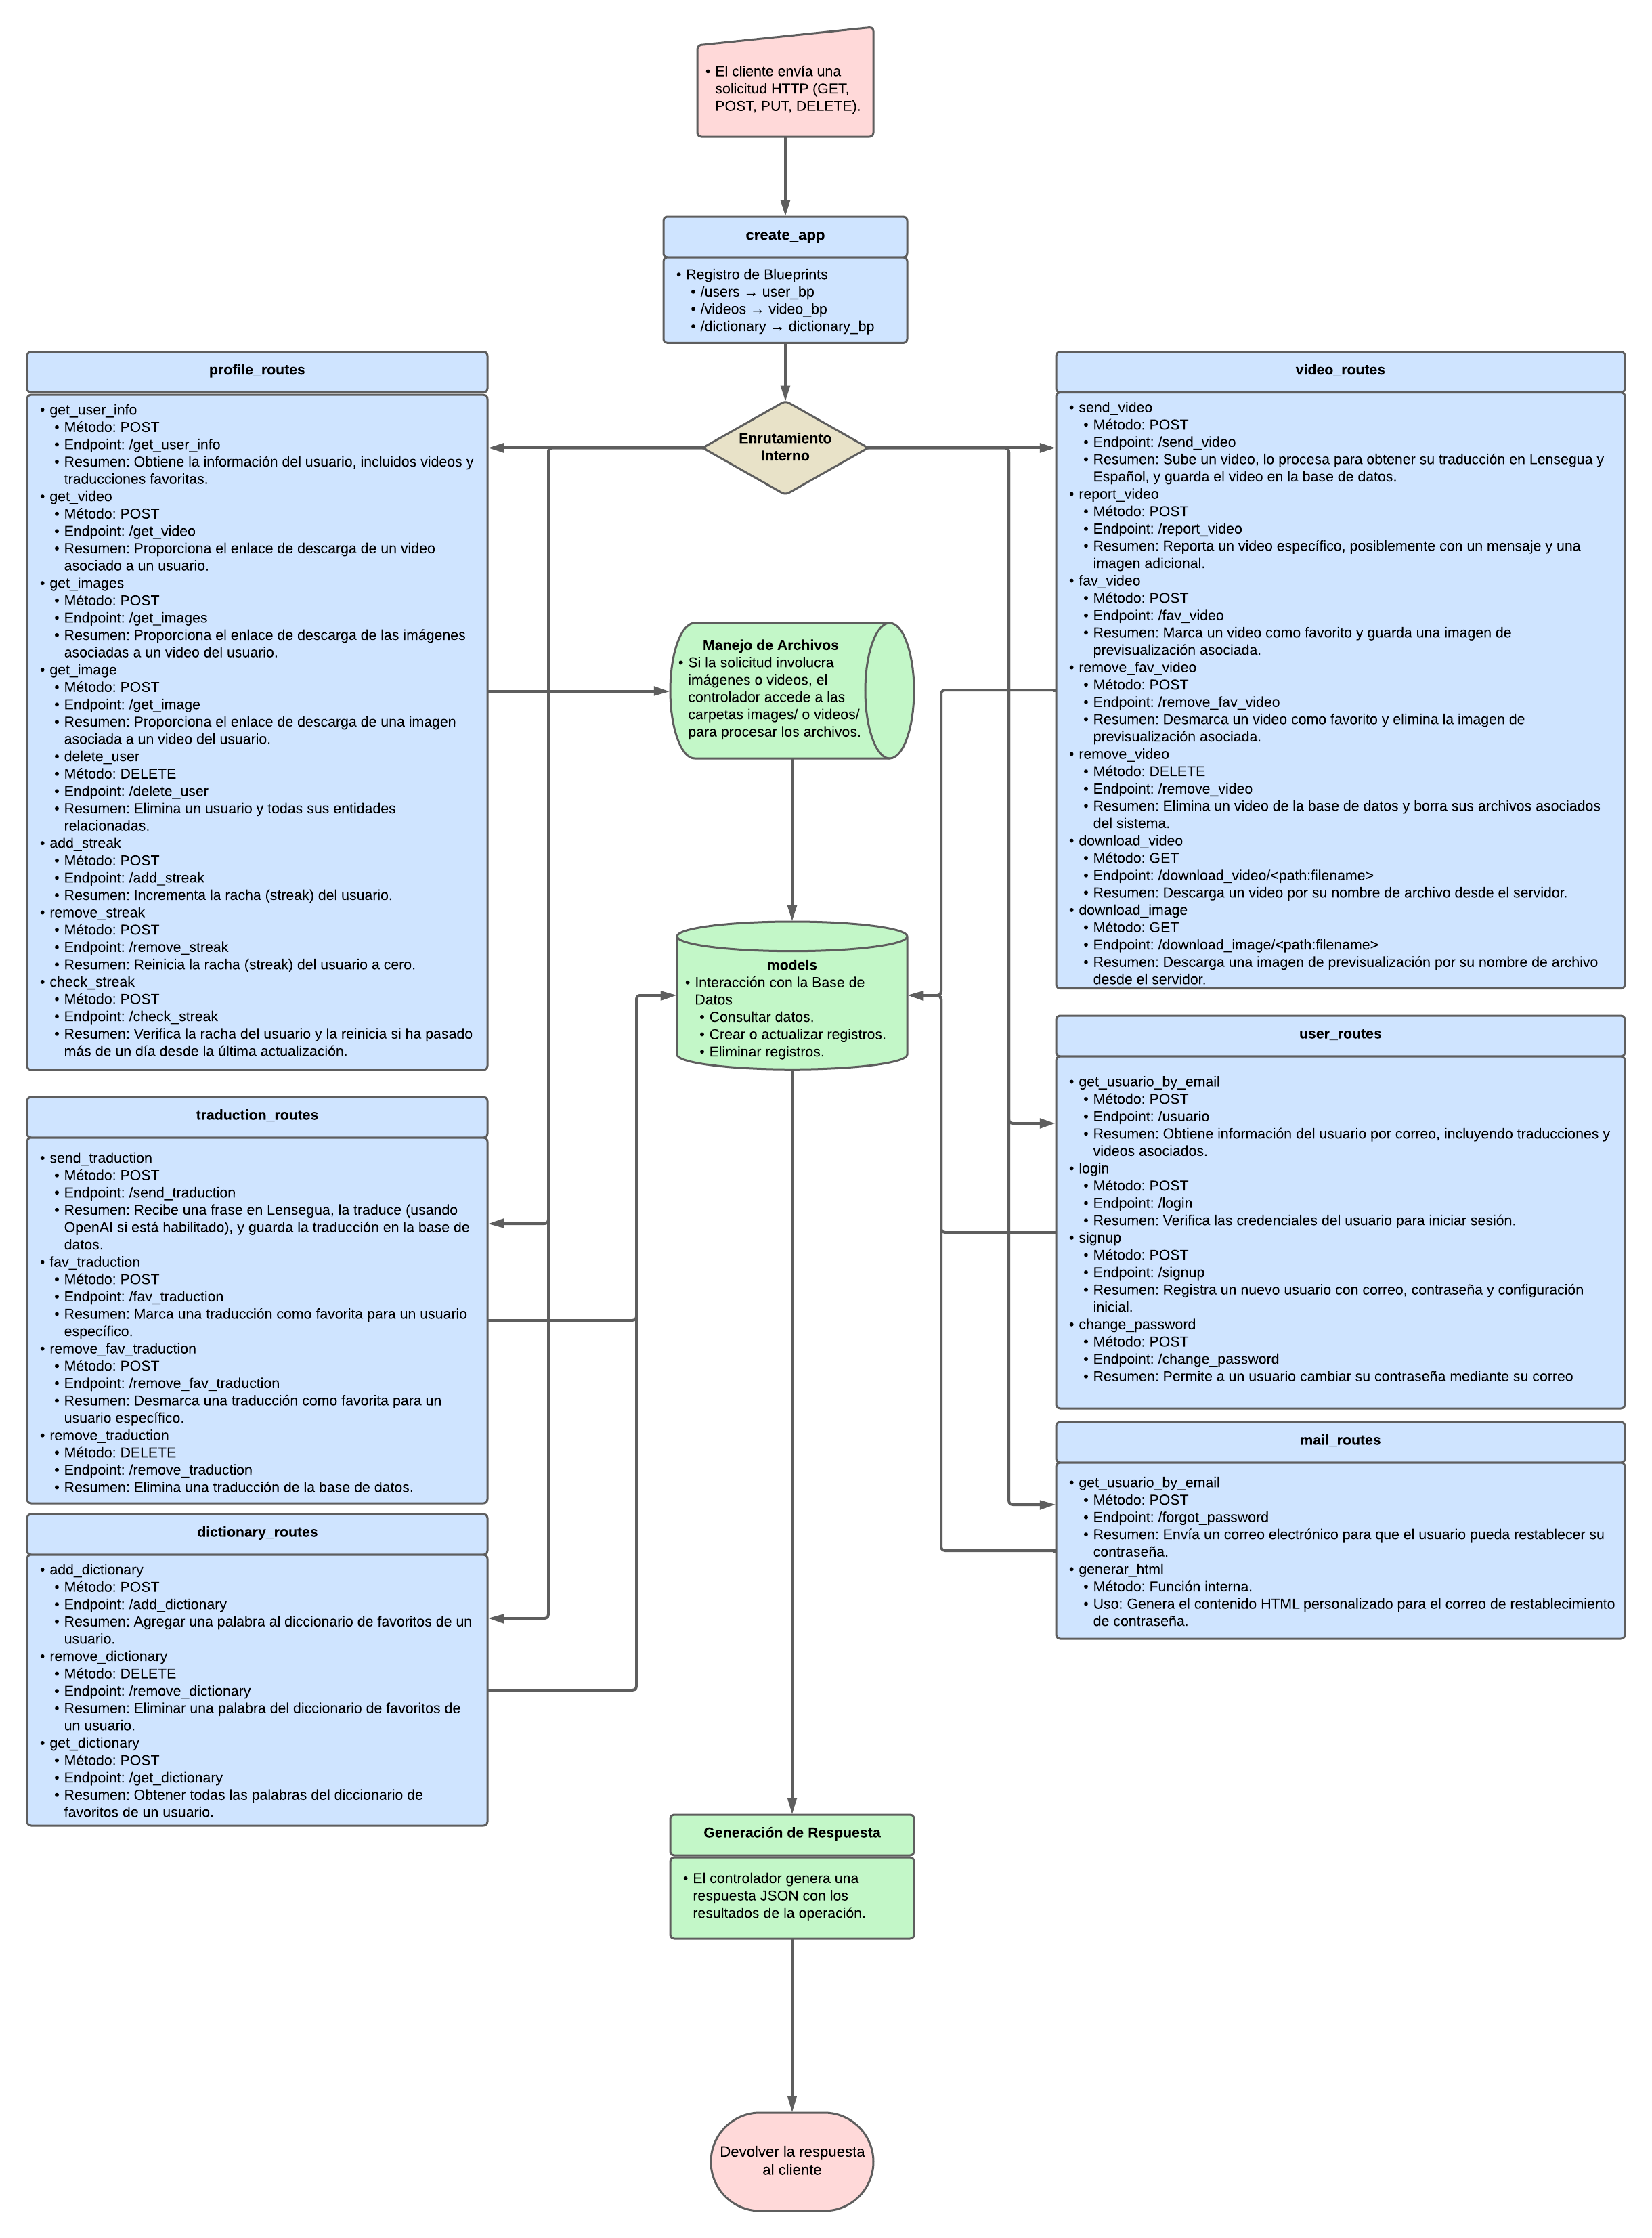
\includegraphics[width=0.5\textwidth]{figuras/diagrama_flujo.png}
    \caption{Diagrama de flujo.}
    \label{fig:diagrama_flujo}
\end{figure}

%Aqui vamos a meter lo del status y como el hacer el inicio del sistema de api-central que pues aqui se resume bien chilero y meter imagen de api-centralServiceStatus

\subsubsection{Implementación de Flask con GUnicorn y NGinx}

% Configuración para resaltar el código de Nginx
\lstset{
    basicstyle=\ttfamily,
    keywordstyle=\color{blue},
    frame=single,
    numbers=left,
    numberstyle=\tiny,
    breaklines=true,
    backgroundcolor=\color{gray!10}
}

% img: DiagramaImplementacionGU-NG.png
\subsubsection*{Componentes principales}

\begin{enumerate}[label=\alph*)]
    \item \textbf{Flask}: Framework de Python utilizado para construir la lógica de la aplicación.
    \item \textbf{Gunicorn}: Servidor WSGI que ejecuta la aplicación Flask en un entorno de producción.
    \item \textbf{Nginx}: Proxy inverso que maneja las solicitudes del cliente, distribuye la carga, y mejora la seguridad.
\end{enumerate}

\subsubsection*{Flujo de trabajo del sistema de APIs:}

\begin{figure}[H]
    \centering
    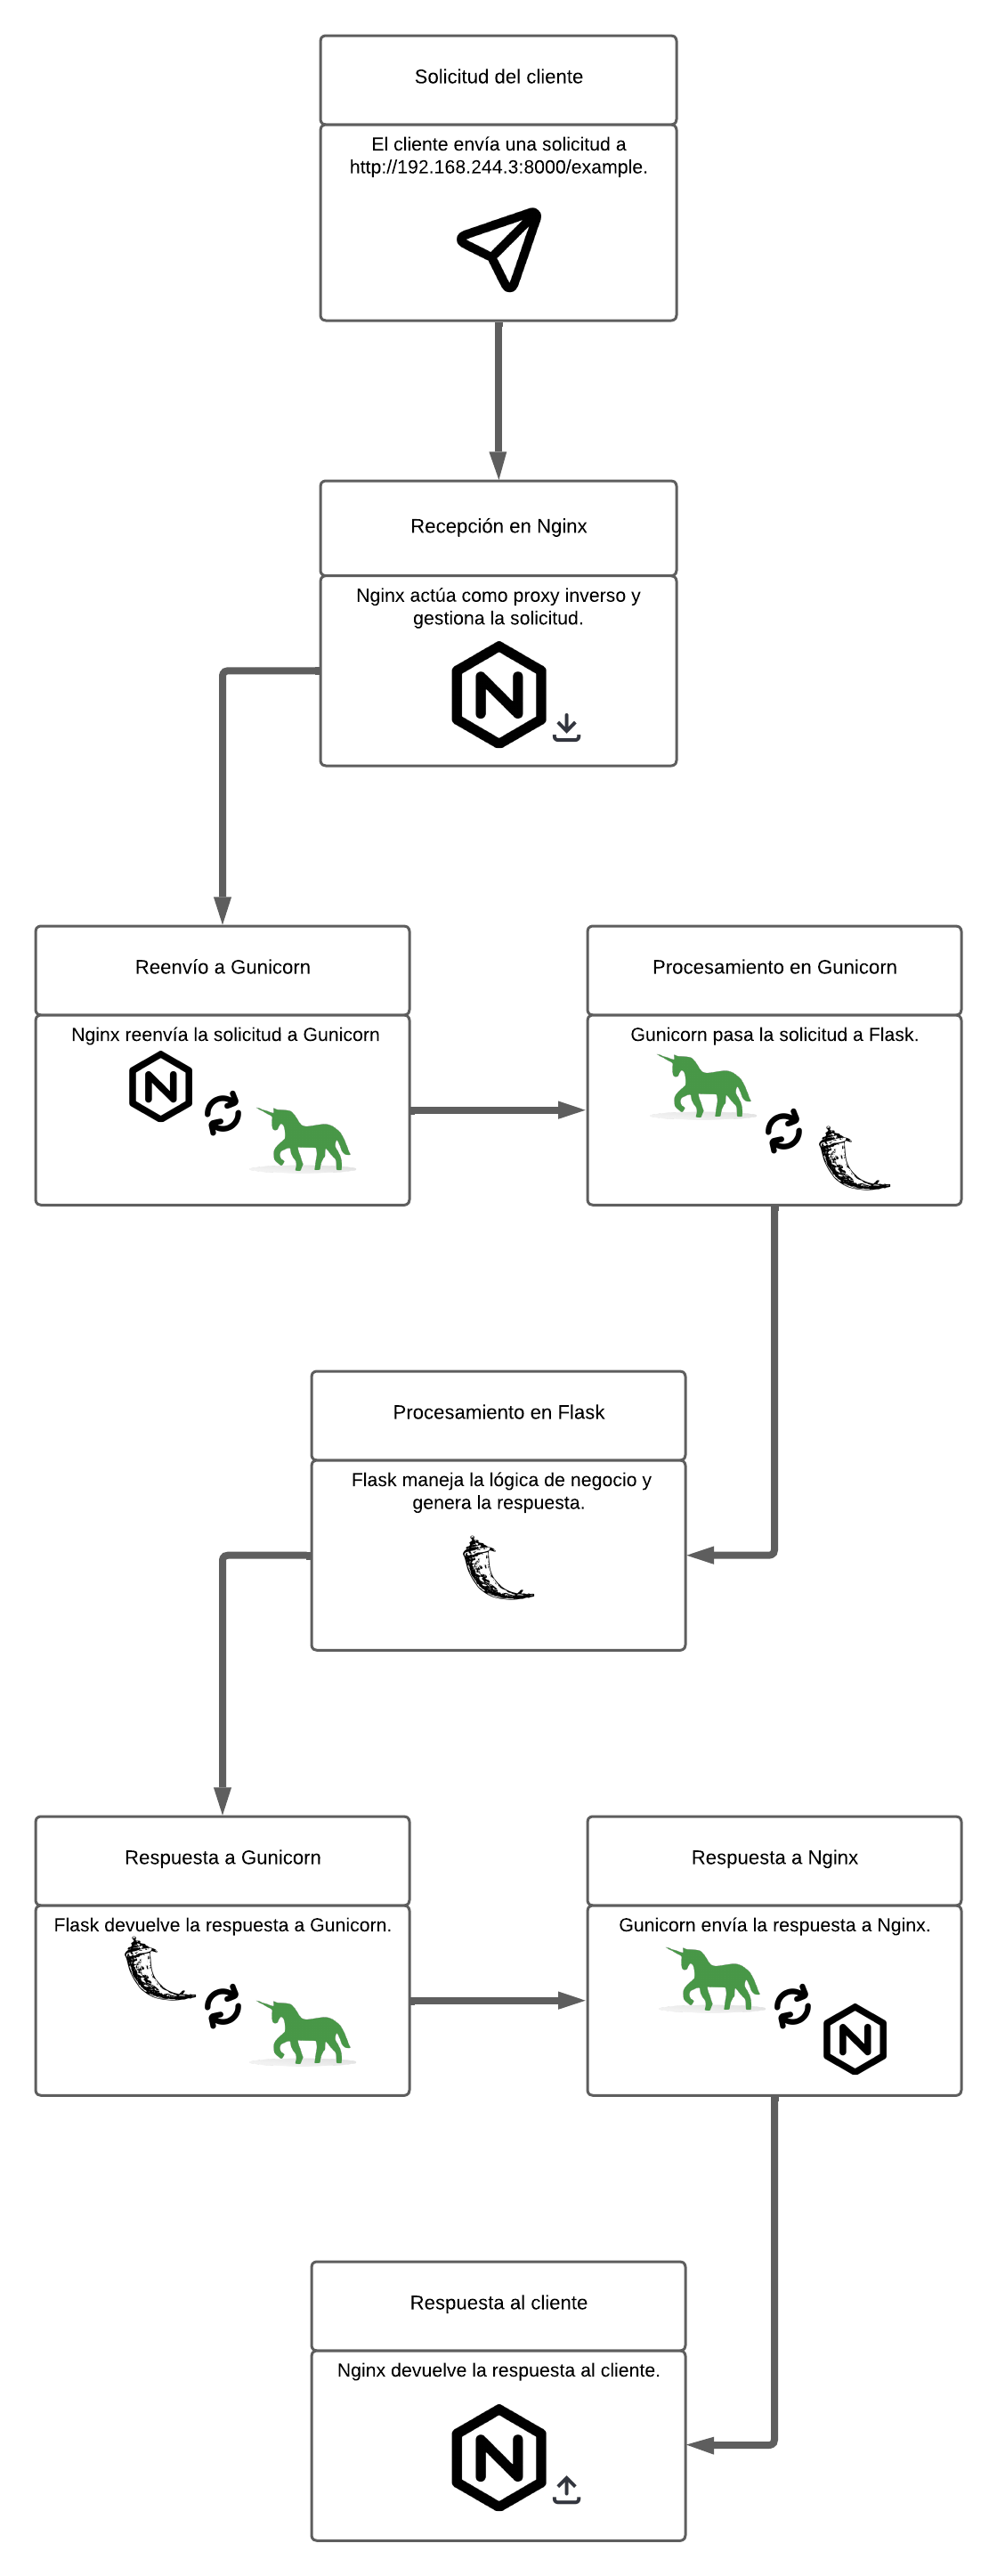
\includegraphics[width=0.5\textwidth]{figuras/DiagramaImplementacionGU-NG.png}
    \caption{Flujo de trabajo completo del sistema de APIs.}
    \label{fig:DiagramaImplementacionGU-NG}
\end{figure}

\subsection*{Configuración general}

\subsubsection*{a. Configuración de Flask}
La aplicación Flask fue configurada con soporte para migraciones de bases de datos, utilizando SQLAlchemy y Flask-Migrate. Esta configuración permite la manipulación sencilla de esquemas de bases de datos a medida que se añaden nuevas funcionalidades al sistema.

\subsubsection*{b. Configuración de Gunicorn}
\begin{enumerate}[label=\roman*.]
    \item Gunicorn se seleccionó como el servidor WSGI debido a su capacidad para manejar múltiples solicitudes concurrentes mediante el uso de workers. Gunicorn se ejecuta vinculándose a todas las interfaces de red en un puerto específico, lo que permite que la aplicación esté disponible en la red local o en internet.
    \item Para gestionar múltiples procesos de Gunicorn, se configuró su ejecución como un servicio del sistema. Esto asegura que Gunicorn inicie automáticamente con el sistema y facilite la gestión del servidor en producción.
\end{enumerate}

\subsubsection*{c. Configuración de Nginx}
\begin{enumerate}[label=\roman*.]
    \item Nginx se configuró como un proxy inverso para manejar la entrada de solicitudes del cliente y distribuirlas a Gunicorn. Este paso es crucial para manejar eficientemente la concurrencia y asegurar que el tráfico de red no sobrecargue el servidor de aplicaciones.
\end{enumerate}

\subsubsection*{d. Archivo de configuración de Nginx:}

\begin{lstlisting}[language=bash, caption={Archivo de configuración de Nginx.}]
server {
    listen 4242;
    server_name 192.168.244.3;

    location / {
        proxy_pass http://unix:/srv/web-apps/api-central/api-central.sock;
        include proxy_params;
        proxy_redirect off;
    }
}
\end{lstlisting}

\subsubsection*{Explicación del archivo de configuración de Nginx:}

\begin{enumerate}[label=\roman*.]
    \item \textbf{listen 4242}: Especifica el puerto en el que Nginx escuchará las solicitudes.
    \item \textbf{server\_name 192.168.244.3}: Define la dirección IP del servidor.
    \item \textbf{proxy\_pass}: Redirige las solicitudes recibidas a Gunicorn mediante un socket Unix, lo que mejora el rendimiento y la seguridad al evitar conexiones TCP adicionales.
    \item \textbf{include proxy\_params}: Incluye parámetros comunes para proxies inversos en Nginx.
    \item \textbf{proxy\_redirect off}: Desactiva la redirección automática de respuestas, permitiendo un control más preciso sobre el flujo de la solicitud y respuesta.
\end{enumerate}

\subsubsection{Implementación de SQLAlchemy para manejo de base de datos y entidades}

% AQUI: colocar imagen de migracionSqlAlchemy

\paragraph*{1. Definición de entidades}
Las entidades en SQLAlchemy se definen como clases que heredan de \texttt{db.Model}. Cada clase representa una tabla en la base de datos, y sus atributos corresponden a las columnas de la tabla. Por ejemplo, una entidad \texttt{Usuario} se define para representar la tabla \texttt{usuarios} con columnas como \texttt{id}, \texttt{correo} y \texttt{contrasena}. Estas clases se definen en un archivo específico, como \texttt{models.py}, para mantener el código organizado y escalable.

\paragraph*{2. Relación entre entidades}
SQLAlchemy permite definir relaciones entre entidades usando claves foráneas (\textit{ForeignKey}). Por ejemplo, en la entidad \texttt{Video}, existe una relación con la entidad \texttt{Usuario} mediante la columna \texttt{usuario\_id}, que referencia al \texttt{id} de la tabla \texttt{usuarios}. Este tipo de relaciones permiten manejar estructuras de datos más complejas y realizar consultas entre tablas relacionadas de forma sencilla.

\paragraph*{3. Migraciones de base de datos}
Flask-Migrate se utiliza para aplicar cambios en el esquema de la base de datos de manera controlada. Una vez que las entidades están definidas, Flask-Migrate permite generar y aplicar migraciones para reflejar estos modelos en la base de datos. Este proceso se realiza en tres pasos:

\begin{enumerate}[label=\alph*.]
    \item \textbf{Inicialización de las Migraciones}: Se configura Flask-Migrate para gestionar la base de datos.
    \item \textbf{Creación de Migraciones}: Cada vez que se añade o modifica una entidad, se genera una nueva migración.
    \item \textbf{Aplicación de Migraciones}: Las migraciones se aplican a la base de datos, creando o modificando las tablas según sea necesario.
\end{enumerate}

\paragraph*{4. Operaciones CRUD}
Con SQLAlchemy, las operaciones CRUD (Crear, Leer, Actualizar, Eliminar) se manejan fácilmente mediante el uso de sesiones de base de datos. Estas sesiones permiten realizar consultas, insertar nuevos registros, actualizar datos existentes y eliminar registros, todo de una manera declarativa y fluida.

\subsubsection{Implementación de módulo API para bases de datos}

Para facilitar las consultas y las inserciones de datos, se utilizará Flask como framework principal debido a su ligereza y capacidad para manejar peticiones de manera eficiente. Este módulo API permitirá un manejo flexible de diferentes formatos de datos, incluyendo videos y texto. La estructura del módulo está diseñada para optimizar el rendimiento del sistema, minimizando el uso de recursos y maximizando la velocidad de respuesta, lo que es crucial para procesar y responder a las interacciones de los usuarios en tiempo real.

% Detalle de las APIs en formato de lista
\textbf{Módulo: Procesamiento de lenguaje}
\begin{itemize}
    \item \textbf{Nombre de la API}: \texttt{API\_Procesamiento\_de\_Lenguaje}
    \item \textbf{Función de la API}: Procesar texto y generar respuestas basadas en el modelo
    \item \textbf{Entrada}: XML con texto
    \item \textbf{Salida Esperada}: Respuesta en XML del modelo GPT-4
\end{itemize}

\textbf{Módulo: Llama}
\begin{itemize}
    \item \textbf{Nombre de la API}: \texttt{API\_Llama}
    \item \textbf{Función de la API}: Analizar y responder consultas con el modelo Llama
    \item \textbf{Entrada}: XML con consulta
    \item \textbf{Salida Esperada}: Respuesta en XML del modelo Llama
\end{itemize}

\textbf{Módulo: Visión por computadora}
\begin{itemize}
    \item \textbf{Nombre de la API}: \texttt{API\_Vision}
    \item \textbf{Función de la API}: Analizar imágenes y videos, y detectar objetos
    \item \textbf{Entrada}: XML con imagen/video
    \item \textbf{Salida Esperada}: Respuesta en XML con análisis de visión por computadora
\end{itemize}

\textbf{Módulo: HyperVisor}
\begin{itemize}
    \item \textbf{Nombre de la API}: \texttt{API\_HyperVisor}
    \item \textbf{Función de la API}: Gestionar y monitorizar las máquinas virtuales
    \item \textbf{Entrada}: XML con comandos
    \item \textbf{Salida Esperada}: Respuesta en XML con estado de VMs
\end{itemize}

\subsubsection{API para integración de modelos de procesamiento}

Se desarrollará una API específica para facilitar la interacción entre el módulo de visión por computadora y los modelos de lenguaje natural. Esta API asegurará que la información fluya de manera eficiente desde la recepción de videos hasta la entrega de resultados en texto o voz, pasando por la consulta de bases de datos. La arquitectura de red y del servidor será diseñada para manejar altas demandas de solicitudes sin degradar la calidad del servicio, utilizando técnicas de balanceo de carga y optimización de recursos para garantizar un proceso robusto y confiable.

Se diseñará un entorno virtualizado utilizando Multipass sobre un servidor con Ubuntu 22.08 ya instalado, lo que facilitará la segregación de los módulos de visión por computadora, inteligencia artificial con GPT-4 y el modelo de IA Llama. Cada uno de estos módulos operará dentro de su propia máquina virtual, configurada específicamente para satisfacer sus requisitos operativos y de procesamiento.

Para iniciar el proceso, se configurarán máquinas virtuales individuales para cada módulo bajo el hypervisor Multipass en Ubuntu 22.08. Esta configuración implica la asignación de los recursos necesarios, como CPU dedicada, memoria RAM adecuada y espacio de almacenamiento suficiente, de acuerdo con las demandas específicas de cada aplicación. Además, se establecerán redes virtuales que permitan una comunicación eficaz y segura entre las máquinas virtuales y los sistemas de bases de datos externos.

\subsubsection{Implementación de Crontab}

Para garantizar que los usuarios mantengan una racha activa y que se reinicie automáticamente si ha pasado más de un día sin actividad, se ha implementado un proceso automatizado utilizando `crontab` en el servidor Linux. Esta tarea se ejecuta todos los días a las 3:00 a.m. y ejecuta un script de Python que revisa la última hora de actualización de la racha de cada usuario y la reinicia si ha pasado más de 24 horas desde la última actualización.

\paragraph{Configuración del Cron Job}

Para configurar la tarea programada que se ejecuta a las 3:00 a.m. todos los días, se debe agregar la siguiente línea al archivo de crontab del usuario adecuado:

\lstset{
    basicstyle=\ttfamily\small,
    numbers=left,
    numberstyle=\tiny\color{gray},
    backgroundcolor=\color{lightgray!20},
    frame=single,
    captionpos=b,
    breaklines=true,
    tabsize=4,
    showstringspaces=false
}

\begin{lstlisting}[caption={Frecuencia de ejecución}, label={lst:cron_frequency}]
0 3 * * *
\end{lstlisting}
\noindent
Indica la frecuencia de ejecución (todos los días a las 3:00 a.m.).

\begin{lstlisting}[caption={Ruta al intérprete de Python}, label={lst:python_path}]
/usr/bin/python3
\end{lstlisting}
\noindent
Es la ruta al intérprete de Python.

\begin{lstlisting}[caption={Ruta al script de Python}, label={lst:script_path}]
/ruta/al/script/reset_streaks.py
\end{lstlisting}
\noindent
Es la ruta completa al script de Python que contiene la lógica de reinicio de rachas.

\begin{lstlisting}[caption={Redirección de salida y errores}, label={lst:log_redirection}]
>> /ruta/al/log/reset_streaks.log 2>&1
\end{lstlisting}
\noindent
Redirige la salida y los errores del script a un archivo de log para facilitar la revisión de su ejecución.

El script de Python que se ejecuta está diseñado para realizar las siguientes tareas:
\begin{enumerate}
    \item Crear una aplicación Flask y un contexto de aplicación para que el script pueda interactuar con la base de datos.
    \item Obtener todos los usuarios de la base de datos y revisar su última hora de actualización de racha.
    \item Calcular la diferencia de tiempo entre la hora actual y la última actualización. Si ha pasado más de 24 horas, reiniciar la racha del usuario y actualizar la hora de la última modificación.
    \item Registrar la acción en la base de datos y mostrar un mensaje de confirmación en la consola.
\end{enumerate}

\noindent
El código del script es el siguiente:

\lstset{
    language=Python,
    basicstyle=\ttfamily\small,
    numbers=left,
    numberstyle=\tiny\color{gray},
    backgroundcolor=\color{lightgray!20},
    frame=single,
    captionpos=b,
    breaklines=true,
    tabsize=4,
    showstringspaces=false
}

\begin{lstlisting}[caption={Script de restablecimiento de streaks en Flask}, label={lst:reset_streaks}]
from app import create_app, db
from app.models import User
from datetime import datetime, timedelta

// Crear la aplicación Flask y contexto
app = create_app()
app.app_context().push()

def reset_streaks():
    // Obtener todos los usuarios
    users = User.query.all()
    for usuario in users:
        if usuario.last_streak_update:
            // Calcular la diferencia de tiempo desde la última actualización
            delta = datetime.utcnow() - usuario.last_streak_update
            if delta > timedelta(days=1):
                // Ha pasado más de un día, reiniciar el streak
                usuario.streak = 0
                usuario.last_streak_update = datetime.utcnow()
                db.session.commit()
                print(f"Streak reset for user {usuario.mail}")

if __name__ == "__main__":
    reset_streaks()
\end{lstlisting}

\paragraph{Importancia de la implementación}

El uso de `crontab` para esta tarea es fundamental para mantener la consistencia y la precisión en el control de rachas de los usuarios sin intervención manual. Esto garantiza que las rachas de los usuarios se gestionen de manera automatizada, promoviendo un comportamiento constante y ofreciendo una mejor experiencia de usuario. Además, el uso de `crontab` permite que la tarea se ejecute en horarios de baja actividad del servidor, minimizando el impacto en el rendimiento del sistema.


\subsection{Virtualización del servidor para múltiples modelos}

\subsection*{Implementación de arquitectura con máquinas virtuales}

Para implementar esta arquitectura, se crearán un total de tres máquinas virtuales adicionales al servidor principal que actuará como HOST. Cada máquina virtual será dedicada a uno de los módulos: visión por computadora, inteligencia artificial con GPT-4 y el modelo de IA Llama.

Utilizando Multipass sobre Ubuntu 22.08, cada máquina virtual se configurará meticulosamente para cumplir con los requisitos específicos de procesamiento, asignando CPU dedicadas, memoria RAM adecuada y espacio de almacenamiento suficiente. Además, se establecerán redes virtuales para asegurar una comunicación eficiente y segura entre las máquinas virtuales y los sistemas de bases de datos. Esta configuración garantizará que cada módulo opere de manera independiente y óptima, permitiendo un procesamiento robusto y confiable bajo altas demandas de solicitudes sin comprometer la calidad del servicio.

\subsubsection*{Resumen del sistema:}

\renewcommand{\arraystretch}{1.3} % Aumenta la altura de las filas
\begin{table}[H]
\centering
\begin{tabularx}{\textwidth}{|m{4cm}|m{6cm}|m{4cm}|}
\hline
\textbf{Memoria RAM} & \textbf{Espacio en disco} & \textbf{CPU} \\ \hline
Total: 125 GiB & /dev/mapper/ubuntu--vg-ubuntu--lv: 98G total, 19G usado, 75G disponible (20\% uso) & Arquitectura: x86\_64 \\ \hline
Usada: 50 MiB & /dev/sda2: 2.0G total, 253M usado, 1.6G disponible (14\% uso) & CPUs: 32 (Intel(R) Xeon(R) Silver 4216 CPU @ 2.10GHz) \\ \hline
Libre: 75 GiB & /dev/sda1: 1.1G total, 6.1M usado, 1.1G disponible (1\% uso) & Núcleos por CPU: 16 \\ \hline
Disponible: 123 GiB & & Hilos por núcleo: 2 \\ \hline
Swap Total: 8.0 GiB & & Virtualización: VT-x \\ \hline
Swap Usada: 0B & & \\ \hline
\end{tabularx}
\caption{Resumen del sistema}
\label{tab:system_summary}
\end{table}

El uso de técnicas de balanceo de carga y la optimización de recursos serán esenciales para garantizar que el sistema pueda manejar altos volúmenes de solicitudes sin comprometer la calidad del servicio. Cada máquina virtual se configurará con las dependencias y bibliotecas necesarias, garantizando que los módulos de visión por computadora y los modelos de IA operen de manera óptima y confiable dentro de este entorno virtualizado controlado.

Parte de este balanceo implica la distribución de recursos entre las máquinas virtuales. Para esto, se dividieron los recursos entre las máquinas de la siguiente manera:

\renewcommand{\arraystretch}{1.3} % Aumenta la altura de las filas
\begin{table}[H]
\centering
\begin{tabularx}{\textwidth}{|m{4.5cm}|m{4cm}|X|}
\hline
\textbf{Máquina Virtual 1 (VM1)} & \textbf{RAM: 32 GiB} & \textbf{CPUs: 8} \\ \hline
\textbf{Máquina Virtual 2 (VM2)} & \textbf{RAM: 32 GiB} & \textbf{CPUs: 8} \\ \hline
\textbf{Máquina Virtual 3 (VM3)} & \textbf{RAM: 32 GiB} & \textbf{CPUs: 8} \\ \hline
\textbf{Host (host de VM)} & \textbf{RAM: 30 GiB (restante)} & \textbf{CPUs: 8 (restante)} \\ \hline
\end{tabularx}
\caption{Distribución de recursos entre las máquinas virtuales y el host}
\label{tab:vm_resources}
\end{table}

\vspace{0.5cm}

\begin{figure}[H]
    \centering
    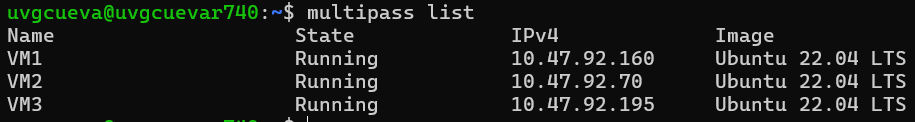
\includegraphics[width=0.5\textwidth]{figuras/EstadosVMs.png}
    \caption{Estado de las máquinas virtuales dentro del sistema}
    \label{fig:EstadosVMs}
\end{figure}

\subsection{Implementación de pruebas de eficiencia}

\begin{enumerate}
    \item \textbf{Instalación de Herramientas de Monitoreo:}
    \begin{enumerate}[label*=\alph*.]
        \item Instalar el agente NGINX Amplify para monitorear el uso de recursos (CPU, memoria, disco y red) en tiempo real.
        \item Adicionalmente, instalar herramientas complementarias como \texttt{htop}, \texttt{dstat}, \texttt{iotop}, \texttt{nload} y \texttt{sysdig} para monitoreo detallado y comparación de métricas.
    \end{enumerate}

    \item \textbf{Preparación del Entorno de Pruebas:}
    \begin{enumerate}[label*=\alph*.]
        \item Desarrollar un script en Python que realice solicitudes a las APIs, utilizando librerías como \texttt{requests} para solicitudes HTTP y \texttt{psutil} para monitoreo de recursos.
        \item Configurar el sistema de logging para registrar métricas en un archivo de log y enviar datos al agente NGINX Amplify.
    \end{enumerate}

    \item \textbf{Monitoreo Continuo:}
    \begin{enumerate}[label*=\alph*.]
        \item Monitorizar los recursos del sistema en tiempo real utilizando NGINX Amplify y las herramientas complementarias instaladas.
        \item Registrar métricas clave como el uso de CPU, memoria, disco y red durante las pruebas.
        \item Configurar alertas en NGINX Amplify para notificaciones automáticas sobre uso excesivo de recursos.
    \end{enumerate}

    \item \textbf{Análisis de Resultados:}
    \begin{enumerate}[label*=\alph*.]
        \item Revisar los logs generados durante las pruebas para evaluar el tiempo de respuesta y la utilización de recursos.
        \item Utilizar el panel de NGINX Amplify para analizar métricas históricas y tendencias de rendimiento.
        \item Identificar cuellos de botella y áreas de mejora mediante las métricas y gráficos proporcionados por NGINX Amplify.
    \end{enumerate}

    \item \textbf{Optimización y Repetición de Pruebas:}
    \begin{enumerate}[label*=\alph*.]
        \item Implementar ajustes necesarios en la configuración del servidor y las aplicaciones basados en los resultados del análisis.
        \item Repetir las pruebas para verificar las mejoras en el rendimiento del sistema.
        \item Continuar el ciclo de pruebas y optimización hasta alcanzar un rendimiento óptimo, utilizando NGINX Amplify para validar las mejoras.
    \end{enumerate}
\end{enumerate}

\subsection{Pruebas de carga}

\subsubsection{Objetivo}
El objetivo de las pruebas de carga es evaluar el rendimiento del sistema bajo condiciones de carga esperadas, simulando múltiples usuarios y solicitudes concurrentes para determinar la capacidad del sistema. Estas pruebas permiten identificar posibles áreas de mejora en la infraestructura y el manejo de recursos.

\subsubsection{Procedimiento}
\begin{enumerate}
    \item \textbf{Simulación de Usuarios}: Se desarrolló un script en Python para crear múltiples usuarios simulados. La función \texttt{create\_users} crea registros y datos de autenticación de usuario, almacenándolos para reutilización durante la prueba.
    \item \textbf{Acciones Concurrentes}: Una vez autenticados, cada usuario simulado ejecuta una serie de acciones concurrentes usando \texttt{ThreadPoolExecutor}:
    \begin{itemize}
        \item Obtiene su información de perfil (\texttt{get\_user\_info}).
        \item Incrementa su racha de actividad (\texttt{add\_streak}).
        \item Realiza operaciones de video y traducción (subida de video, recuperación, marcación como favorito).
    \end{itemize}
    \item \textbf{Medición de Tiempos de Respuesta}: La función \texttt{send\_request} mide el tiempo de respuesta de cada operación y el estado HTTP. Esto permite registrar tiempos de respuesta y determinar si el sistema mantiene la estabilidad bajo carga.
\end{enumerate}

Para evaluar la capacidad de nuestro servidor y entender sus límites de rendimiento, realizamos una serie de pruebas de carga incrementales. Estas pruebas consistieron en simular un número creciente de usuarios concurrentes interactuando con el sistema, comenzando con 50 usuarios y aumentando progresivamente hasta 1100 usuarios. El objetivo de este enfoque es aplicar niveles crecientes de estrés en el servidor, analizando cómo responde bajo diferentes cargas de trabajo.

Cada prueba de carga permite observar el tiempo de respuesta y la estabilidad del sistema a medida que la cantidad de usuarios aumenta, identificando el punto en el que el rendimiento empieza a degradarse significativamente. Esta metodología nos ayuda a determinar la capacidad máxima de usuarios concurrentes que nuestro servidor puede manejar de forma estable antes de experimentar problemas críticos, como demoras excesivas o fallos en el procesamiento de las solicitudes. Además, este proceso de pruebas graduales nos permite identificar las métricas críticas que influencian el desempeño, tales como la utilización de CPU, la memoria disponible y el tiempo de respuesta de las solicitudes.

\newpage

%tenemos que cargar las imagenes pruebaCarga50U.png
%tenemos que cargar las imagenes pruebaCarga100U.png
%tenemos que cargar las imagenes pruebaCarga200U.png
%tenemos que cargar las imagenes pruebaCarga300U.png
%tenemos que cargar las imagenes pruebaCarga400U.png
%tenemos que cargar las imagenes pruebaCarga500U.png
%tenemos que cargar las imagenes pruebaCarga600U.png
%tenemos que cargar las imagenes pruebaCarga700U.png
%tenemos que cargar las imagenes pruebaCarga800U.png
%tenemos que cargar las imagenes pruebaCarga900U.png
%tenemos que cargar las imagenes pruebaCarga1100U.png
\begin{figure}[H]
    \centering
    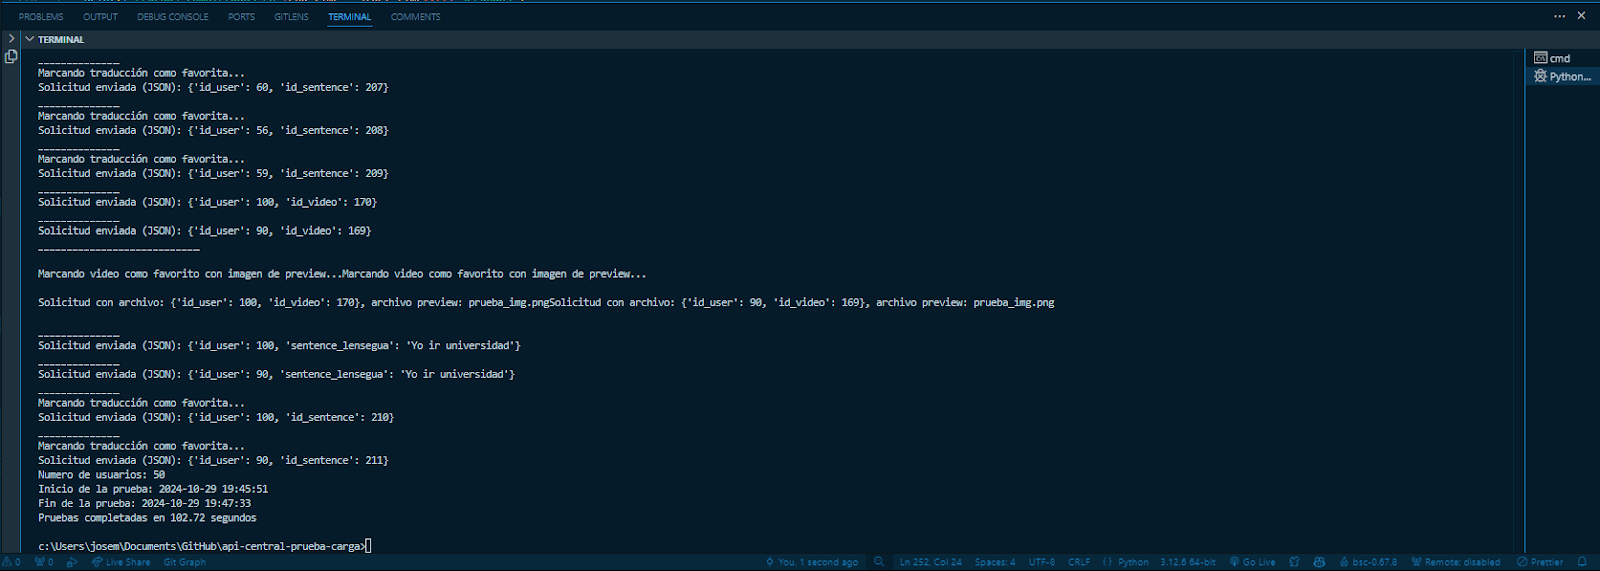
\includegraphics[width=0.5\textwidth]{figuras/pruebaCarga50U.png}
    \caption{Resultados de la prueba de carga con 50 usuarios concurrentes.}
    \label{fig:pruebaCarga50U}
\end{figure}

\begin{figure}[H]
    \centering
    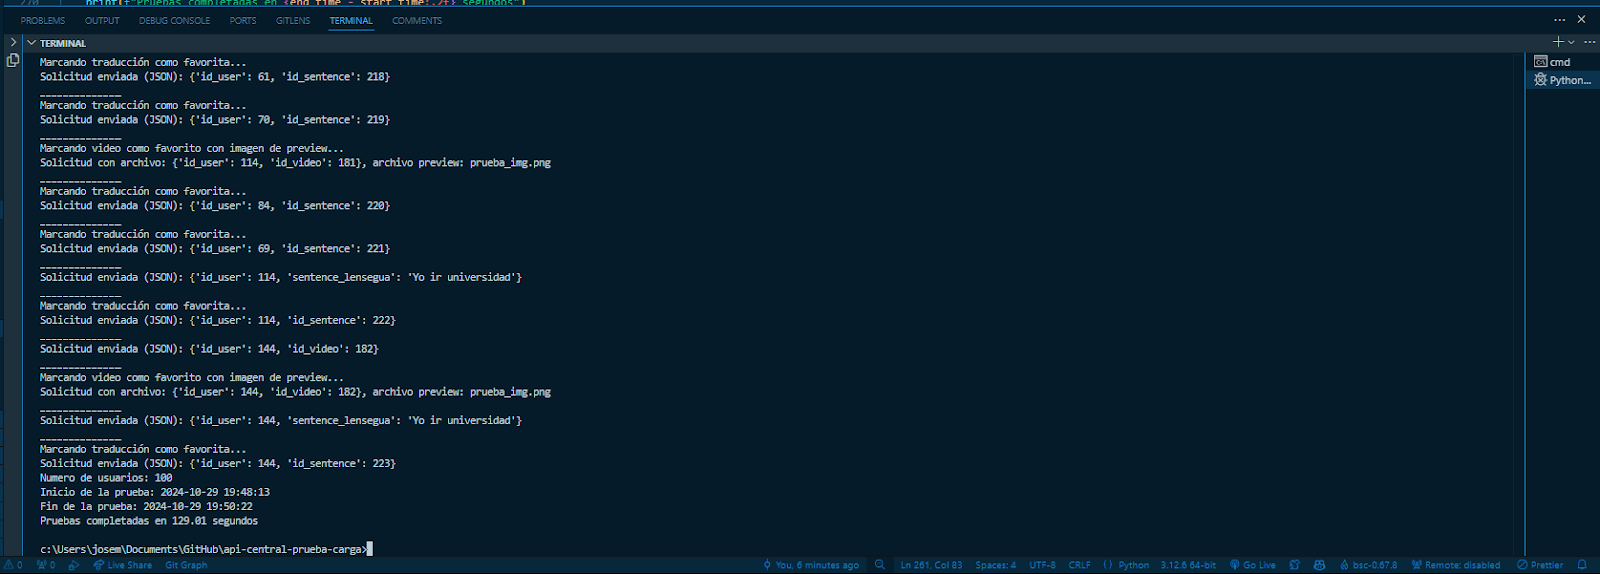
\includegraphics[width=0.5\textwidth]{figuras/pruebaCarga100U.png}
    \caption{Resultados de la prueba de carga con 100 usuarios concurrentes.}
    \label{fig:pruebaCarga100U}
\end{figure}

\begin{figure}[H]
    \centering
    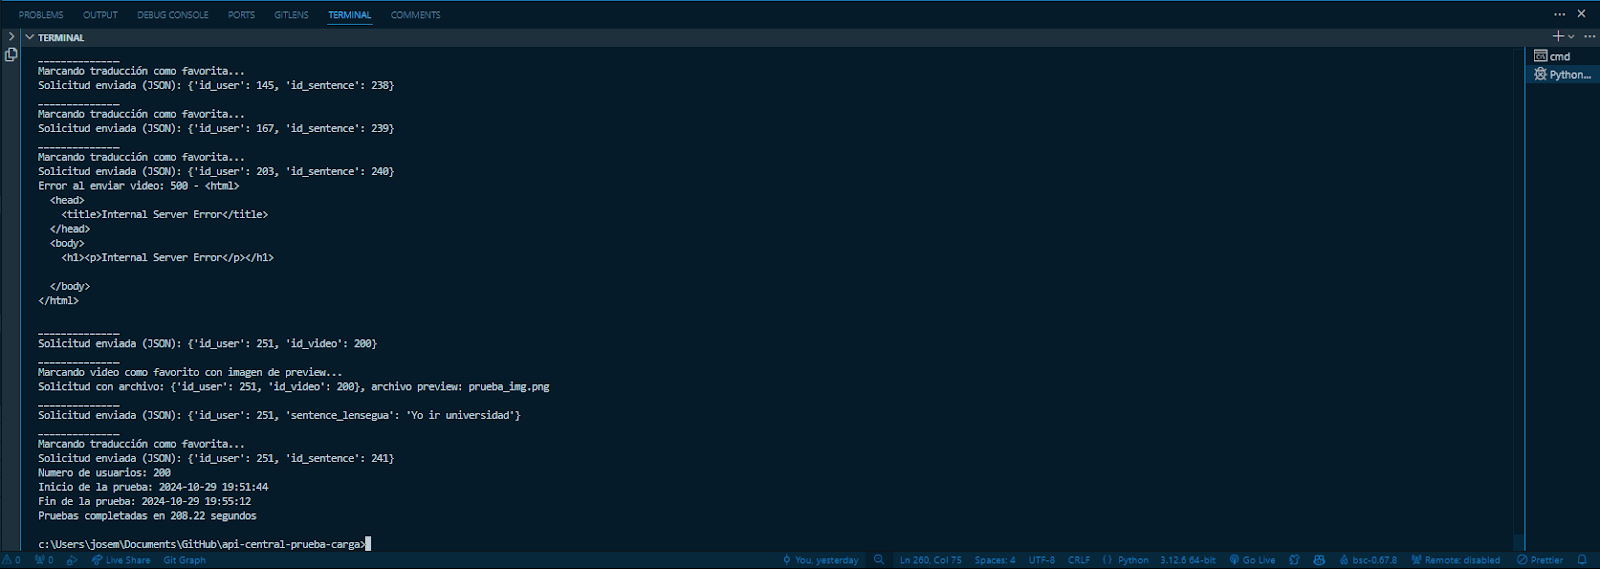
\includegraphics[width=0.5\textwidth]{figuras/pruebaCarga200U.png}
    \caption{Resultados de la prueba de carga con 200 usuarios concurrentes.}
    \label{fig:pruebaCarga200U}
\end{figure}

\begin{figure}[H]
    \centering
    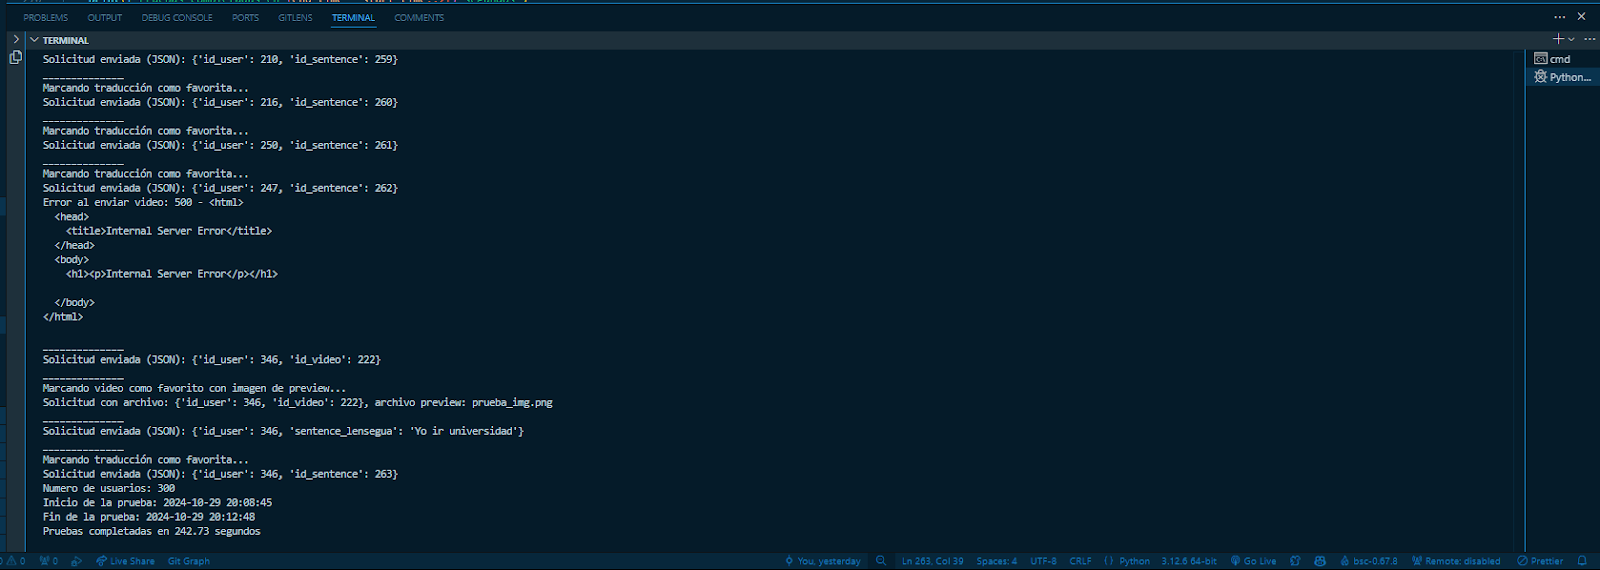
\includegraphics[width=0.5\textwidth]{figuras/pruebaCarga300U.png}
    \caption{Resultados de la prueba de carga con 300 usuarios concurrentes.}
    \label{fig:pruebaCarga300U}
\end{figure}

\begin{figure}[H]
    \centering
    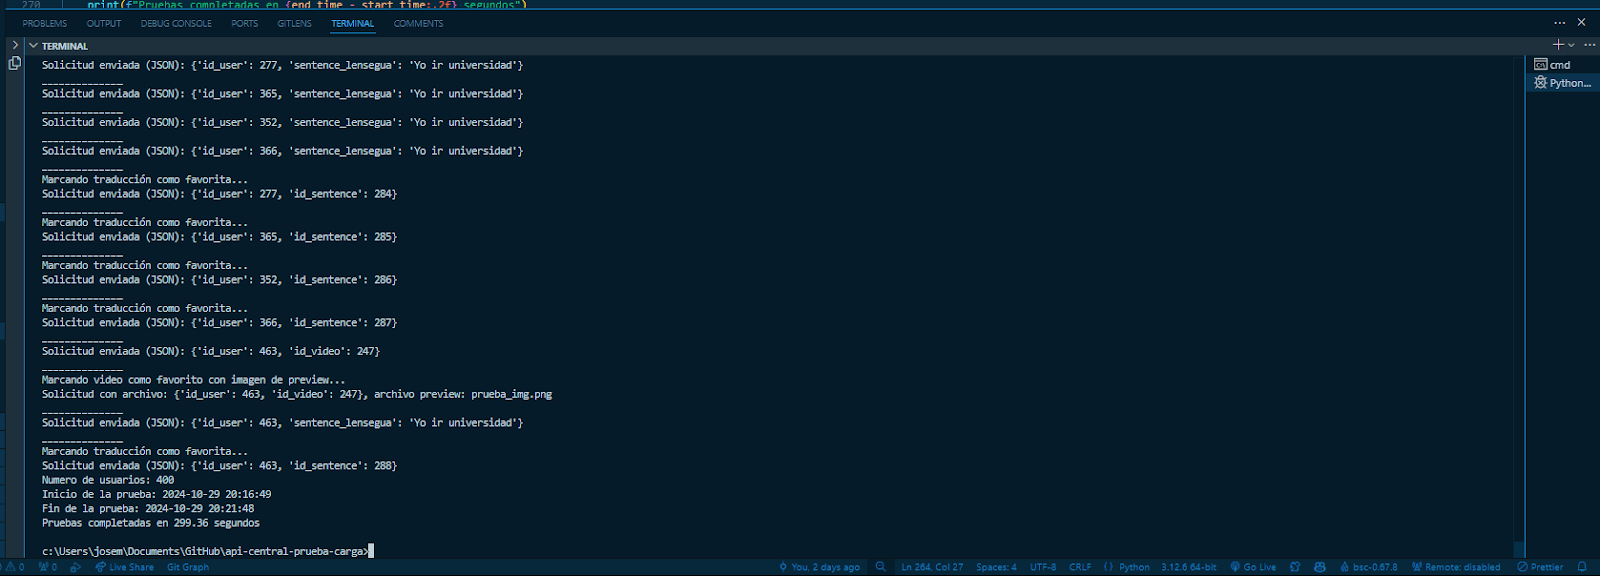
\includegraphics[width=0.5\textwidth]{figuras/pruebaCarga400U.png}
    \caption{Resultados de la prueba de carga con 400 usuarios concurrentes.}
    \label{fig:pruebaCarga400U}
\end{figure}

\begin{figure}[H]
    \centering
    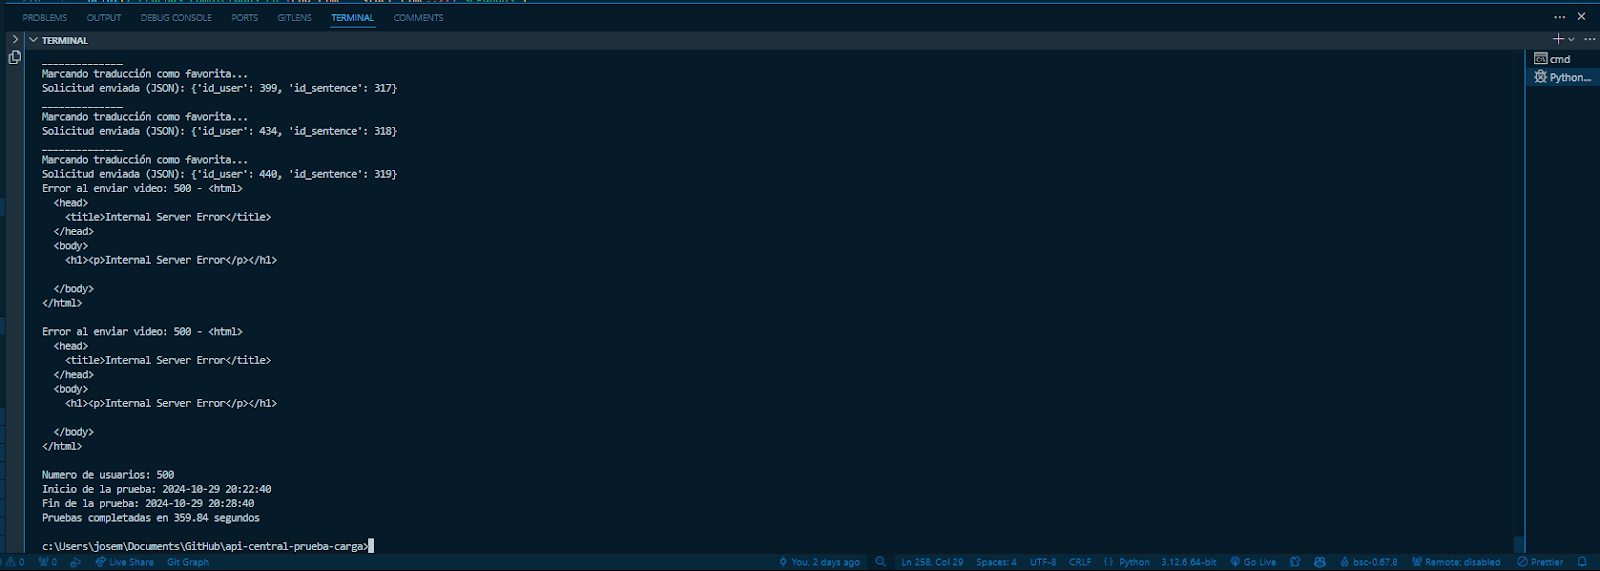
\includegraphics[width=0.5\textwidth]{figuras/pruebaCarga500U.png}
    \caption{Resultados de la prueba de carga con 500 usuarios concurrentes.}
    \label{fig:pruebaCarga500U}
\end{figure}

\begin{figure}[H]
    \centering
    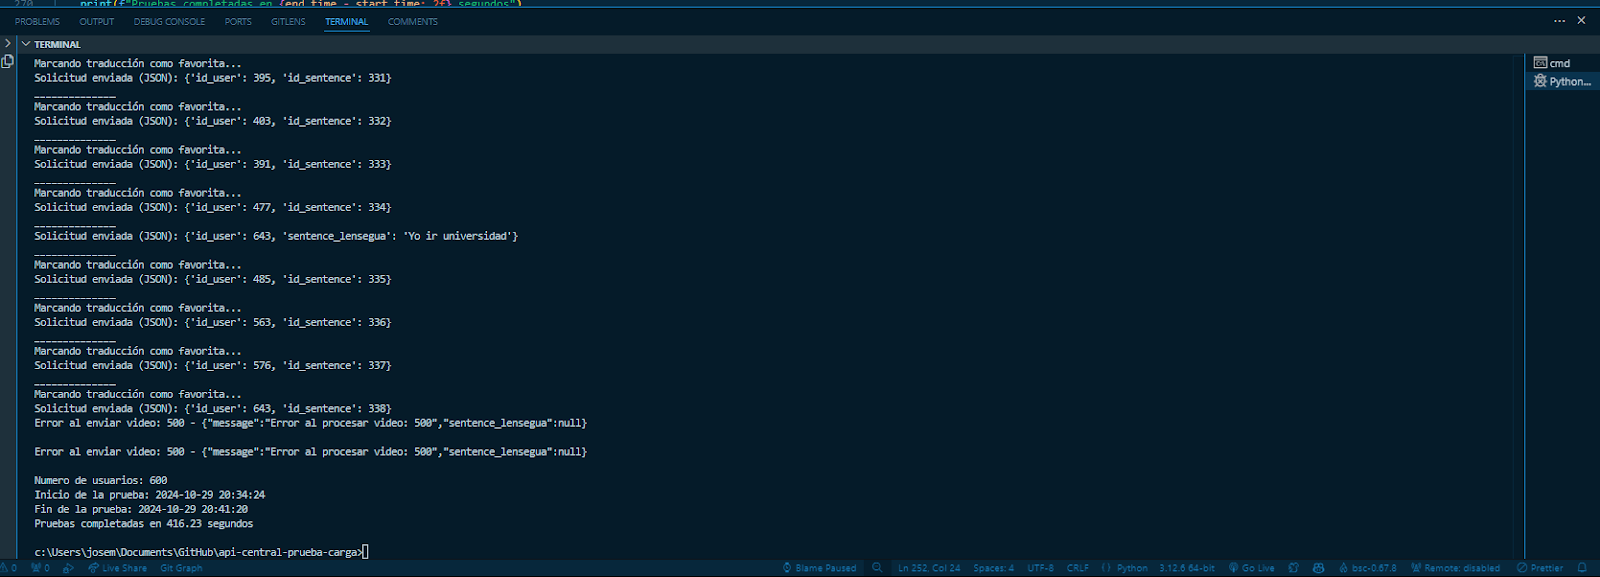
\includegraphics[width=0.5\textwidth]{figuras/pruebaCarga600U.png}
    \caption{Resultados de la prueba de carga con 600 usuarios concurrentes.}
    \label{fig:pruebaCarga600U}
\end{figure}

\begin{figure}[H]
    \centering
    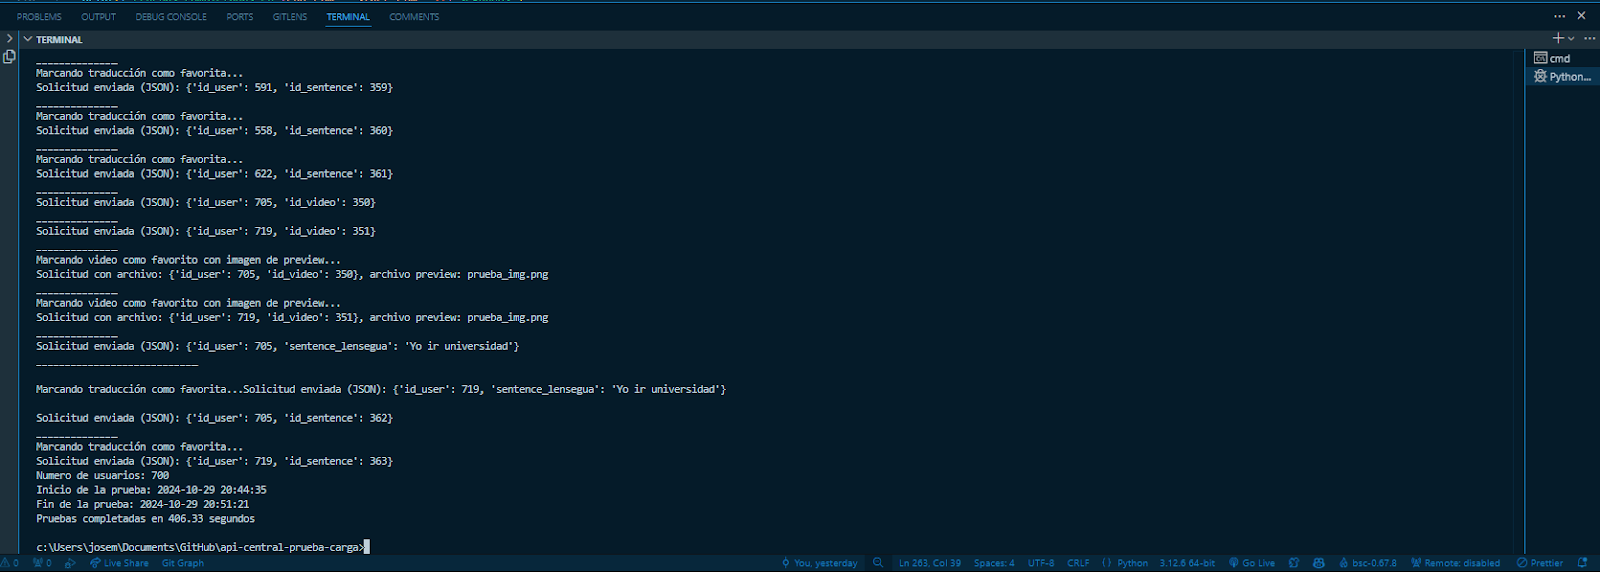
\includegraphics[width=0.5\textwidth]{figuras/pruebaCarga700U.png}
    \caption{Resultados de la prueba de carga con 700 usuarios concurrentes.}
    \label{fig:pruebaCarga700U}
\end{figure}

\begin{figure}[H]
    \centering
    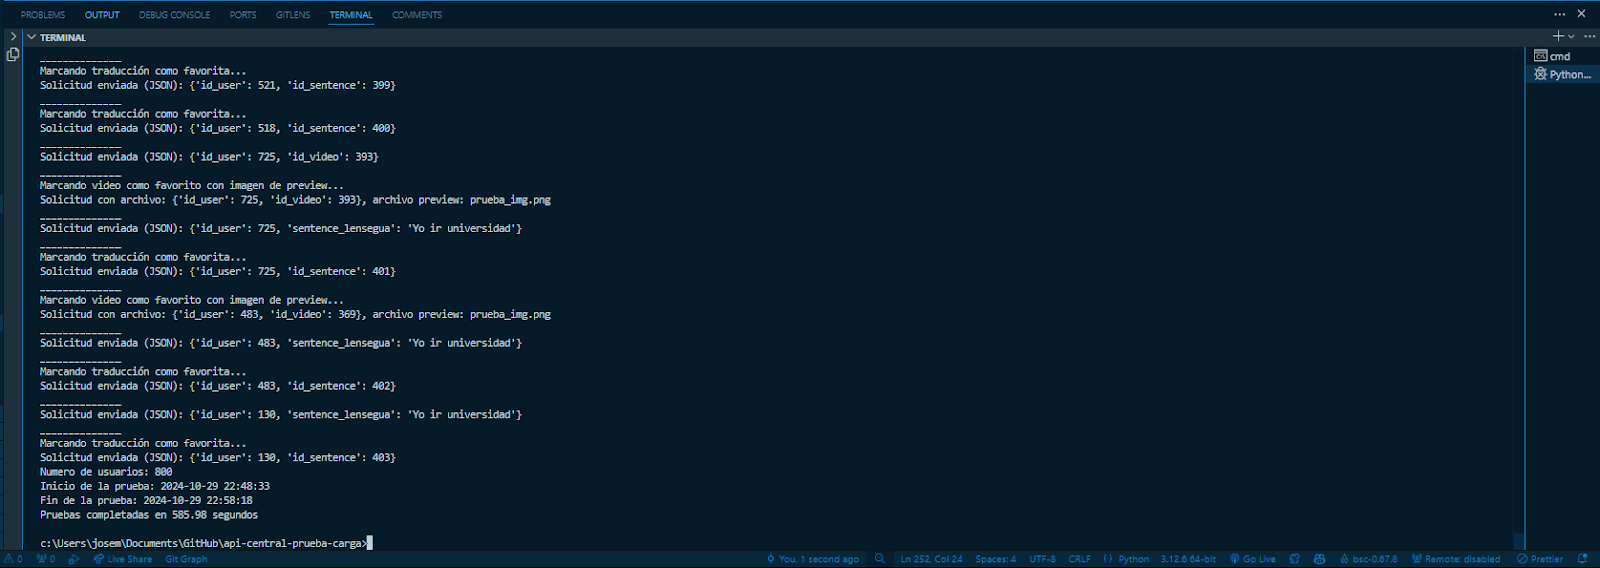
\includegraphics[width=0.5\textwidth]{figuras/pruebaCarga800U.png}
    \caption{Resultados de la prueba de carga con 800 usuarios concurrentes.}
    \label{fig:pruebaCarga800U}
\end{figure}

\begin{figure}[H]
    \centering
    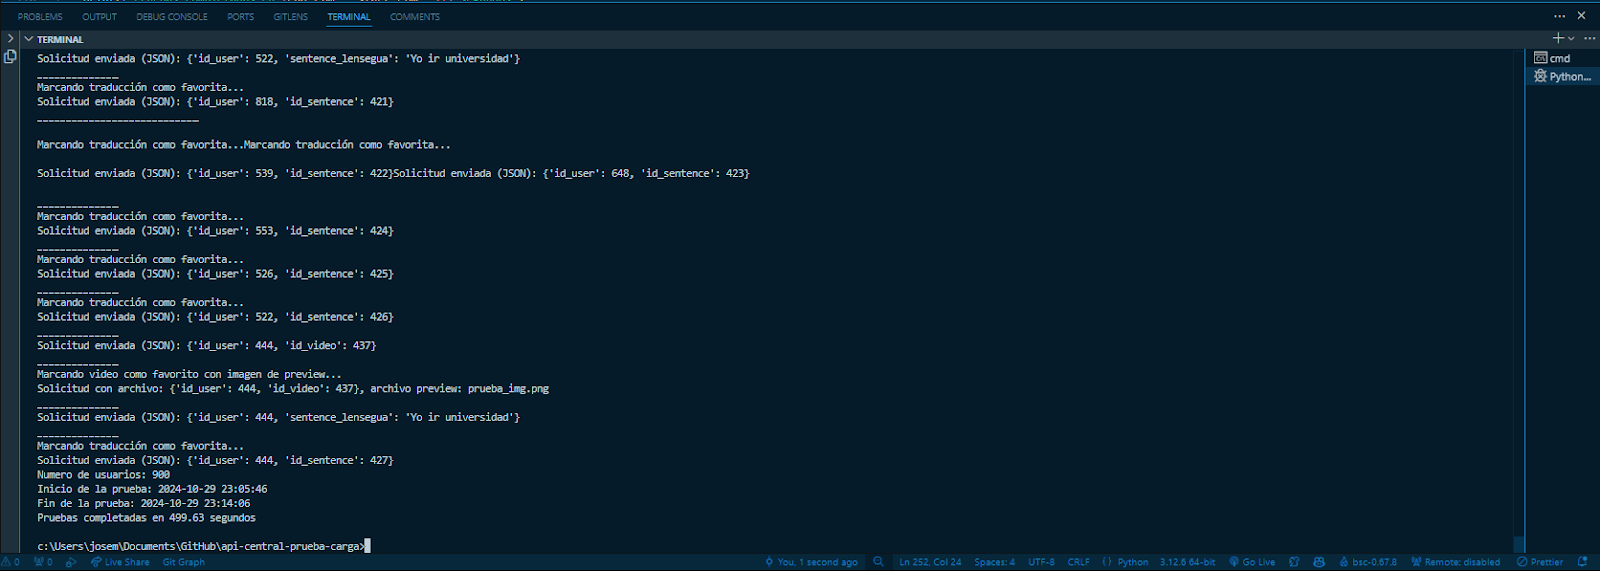
\includegraphics[width=0.5\textwidth]{figuras/pruebaCarga900U.png}
    \caption{Resultados de la prueba de carga con 900 usuarios concurrentes.}
    \label{fig:pruebaCarga900U}
\end{figure}

\begin{figure}[H]
    \centering
    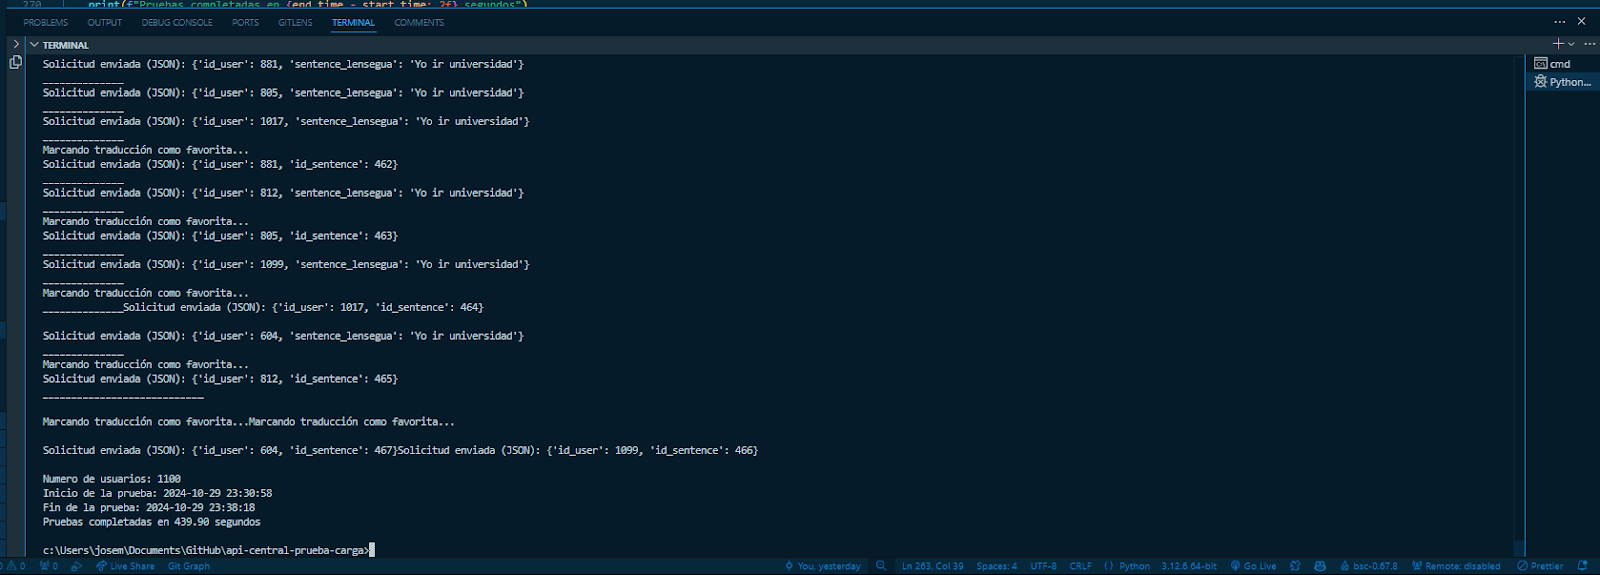
\includegraphics[width=0.5\textwidth]{figuras/pruebaCarga1100U.png}
    \caption{Resultados de la prueba de carga con 1100 usuarios concurrentes.}
    \label{fig:pruebaCarga1100U}
\end{figure}

\subsection{Pruebas de Extremo a Extremo (E2E)}

\subsubsection{Objetivo}
Las pruebas E2E validan el flujo completo de la aplicación desde la perspectiva del usuario, asegurando que todos los módulos y APIs se integren correctamente y que las funciones principales respondan adecuadamente en un flujo de uso continuo.

\subsubsection{Procedimiento}
\begin{enumerate}
    \item \textbf{Flujo Completo del Usuario}: Un usuario simulado realiza una serie de acciones que incluyen:
    \begin{itemize}
        \item Registro y autenticación.
        \item Acceso a su perfil, subida de video, marcación y eliminación de favoritos.
        \item Interacción con el sistema de traducciones y diccionario.
    \end{itemize}
    \item \textbf{Verificación y Tiempo de Respuesta}: Cada acción registra el tiempo de respuesta y verifica que el estado HTTP sea 200 (éxito). Esto garantiza que todas las funcionalidades respondan correctamente en un flujo integrado.
\end{enumerate}

% vamos a cargar la imagen e2e2test.png
La prueba End-to-End (E2E) se diseñó para evaluar el flujo completo de la aplicación desde la perspectiva del usuario, verificando que todas las APIs respondieran correctamente y que las funcionalidades se integraran de manera óptima. 

\subsection{Implementación de pruebas CVE para seguridad}

\begin{enumerate}
    \item \textbf{Identificación de Vulnerabilidades:}
    \begin{enumerate}
        \item Utilizar herramientas de escaneo de vulnerabilidades como Nessus, OpenVAS o Qualys para identificar posibles vulnerabilidades en el sistema.
        \item Asegurarse de que todas las vulnerabilidades identificadas estén referenciadas con sus respectivos identificadores CVE.
    \end{enumerate}
    
    \item \textbf{Evaluación de Vulnerabilidades:}
    \begin{enumerate}
        \item Realizar pruebas exhaustivas de seguridad para obtener los datos necesarios para la calculadora CVSS. Las pruebas incluyen:
        \begin{enumerate}
            \item Pruebas de Explotabilidad: Evaluar cuán fácilmente se puede explotar la vulnerabilidad, incluyendo factores como la complejidad del ataque y los privilegios requeridos.
            \item Pruebas de Impacto: Medir el impacto potencial de la vulnerabilidad en la confidencialidad, integridad y disponibilidad del sistema.
            \item Pruebas de Alcance: Determinar si la vulnerabilidad afecta sólo al componente vulnerable o si se puede propagar a otros componentes.
        \end{enumerate}
        \item Recopilar los datos obtenidos de las pruebas y utilizar una calculadora de puntaje CVE, como la proporcionada por el NVD (National Vulnerability Database), para calcular el puntaje de cada vulnerabilidad basada en los criterios de CVSS (Common Vulnerability Scoring System).
        \item \textbf{Criterios de CVSS:}
        \begin{enumerate}
            \item \textbf{Base Score}: Evaluación del impacto y la facilidad de explotación de la vulnerabilidad.
            \item \textbf{Temporal Score}: Considera factores temporales como la disponibilidad de explotaciones y parches.
            \item \textbf{Environmental Score}: Ajusta el puntaje base según el entorno y la configuración específicos.
        \end{enumerate}
    \end{enumerate}

    \item \textbf{Validación de Medidas de Seguridad:}
    \begin{enumerate}
        \item Implementar y validar las medidas de mitigación necesarias para corregir las vulnerabilidades identificadas.
        \item Realizar pruebas de validación post-mitigación para asegurar que las vulnerabilidades hayan sido corregidas y que las medidas no afecten negativamente el rendimiento del sistema.
    \end{enumerate}

    \item \textbf{Monitoreo Continuo:}
    \begin{enumerate}
        \item Realizar escaneos periódicos de vulnerabilidades para identificar nuevas amenazas y asegurarse de que las vulnerabilidades conocidas estén mitigadas.
        \item Recalcular los puntajes de CVE periódicamente para asegurar que el sistema se mantenga seguro.
    \end{enumerate}

    \item \textbf{Documentación y Reportes:}
    \begin{enumerate}
        \item Mantener un registro detallado de todas las vulnerabilidades identificadas, sus puntajes CVE y las acciones de mitigación realizadas.
        \item Generar reportes periódicos que incluyan análisis de tendencias en las vulnerabilidades y la efectividad de las medidas de seguridad implementadas.
    \end{enumerate}

    \item \textbf{Optimización y Mejora Continua:}
    \begin{enumerate}
        \item Basado en los análisis de vulnerabilidades y puntajes CVE, implementar ajustes necesarios en la configuración del servidor y las aplicaciones.
        \item Repetir las pruebas de seguridad para verificar las mejoras en la protección del sistema.
        \item Continuar el ciclo de pruebas y optimización hasta alcanzar un nivel óptimo de seguridad.
    \end{enumerate}
\end{enumerate}

\subsection{Pruebas de seguridad con Lynis}

\subsubsection{Objetivo}
En este proyecto, se utilizó Lynis para auditar la seguridad del sistema mediante su Índice de Fortalecimiento. Este índice proporcionó una evaluación cuantitativa basada en la implementación de medidas de seguridad y prácticas recomendadas. Para cumplir con los objetivos del sistema, se definió una meta inicial de un puntaje de 40, considerado como la base para garantizar un sistema con medidas de seguridad básicas adecuadas. Este enfoque siguió las recomendaciones de la documentación de Lynis Hardening Index \cite{LynisHardeningIndex}, que establecía que un puntaje de 40 era suficiente para aplicaciones estándar, mientras que resultados más altos reflejaban un sistema más robusto. Según el CIS Benchmark \cite{CISBenchmarksReport}, una auditoría con un puntaje superior a 50 indicaba un fortalecimiento razonable para sistemas en entornos no críticos.

\subsubsection{Procedimiento}
\begin{enumerate}
    \item \textbf{Instalación y Ejecución}: Lynis fue instalado y ejecutado con el siguiente comando:
    \begin{verbatim}
    sudo lynis audit system
    \end{verbatim}
    Al finalizar, Lynis generó un informe con recomendaciones específicas para mejorar la seguridad del sistema.
    
    \item \textbf{Interpretación del Informe}: El informe proporcionado incluyó una puntuación general de seguridad, destacando las áreas de mayor riesgo y ofreciendo recomendaciones detalladas. 
\end{enumerate}

\subsection{Mejoras de seguridad en \texttt{/etc/sysctl.conf}}

En base a las recomendaciones de Lynis, se realizaron ajustes en el archivo \texttt{/etc/sysctl.conf} para mejorar la seguridad de red del sistema. Estas configuraciones incluyen:

\begin{itemize}
    \item \textbf{Deshabilitar redirecciones ICMP} para prevenir ataques de red.
    \item \textbf{Habilitar SYN Cookies} para mitigar ataques SYN flood.
    \item \textbf{Restringir el uso de \texttt{dmesg} para usuarios no privilegiados}.
\end{itemize}

\subsection{Monitoreo continuo de seguridad con ClamAV}

\subsubsection{Instalación y configuración}
ClamAV y su servicio de actualización \textbf{freshclam} fueron instalados para realizar escaneos de seguridad en el sistema de manera regular. Esto garantiza una capa adicional de protección contra amenazas de malware.

\subsubsection{Monitoreo y ajustes adicionales}
El sistema fue configurado para realizar escaneos periódicos y actualizar la base de datos de ClamAV. Esto permite mantener el sistema protegido frente a vulnerabilidades potenciales en el software o archivos nuevos.






































% MODULO DE DISEÑO =============

\section{Diseño y desarrollo móvil}

\subsection{Investigación de mercado}

\subsubsection{Investigación y revisión sobre aplicaciones y tecnologías similares}

Se investigan aplicaciones con funcionalidades parecidas a la solución propuesta por Señas Chapinas. 

\paragraph{Hand Talk Translator}

Es una aplicación gratuita para dispositivos Android e iOS diseñada para mejorar la comunicación entre la comunidad sorda y las personas que pueden oír. Esta traduce texto, ya sea en texto o en audio, al lenguaje de señas americanas. Esto se realiza por medio de Hugo, un avatar tridimensional animado por IA, que facilita la traducción y el aprendizaje. Los usuarios tienen la opción de repetir las traducciones, modificar la velocidad de Hugo, guardar y calificar sus traducciones preferidas. También pueden crear mensajes en GIF para compartir y personalizar la apariencia de Hugo en su tienda \cite{Foggetti2023}.

    
\begin{itemize}
    \item \textbf{Funcionalidades destacadas}
    \begin{itemize}
        \item Traducción de frases a lengua de señas ASL mostrado a través de animación 3D.
        \item Opción de compartir por GIF en redes sociales.
        \item Opción de guardar traducción en favoritos.
        \item Opción de repetir la traducción y cambiar la velocidad de reproducción.
    \end{itemize}
    
    \item \textbf{Características de Diseño}
    \begin{itemize}
        \item Incorpora elementos interactivos y de personalización para mejorar la experiencia del usuario. Esto vuelve la aplicación más atractiva y personal.
        \item Animación fluida de Hugo, que facilita el seguimiento visual de las señas.
        \item Interfaz intuitiva y simple que permite una navegación sencilla por las distintas funciones de la aplicación.
        \item Uso de color naranja que induce calidez, alegría, optimismo y confianza.
        \item Los íconos y botones son grandes y están claramente etiquetados, lo cual es útil para una rápida identificación de la funcionalidad.
        \item La interfaz es responsiva.
    \end{itemize}

    \item \textbf{Comentarios de usuarios}
    \begin{itemize}
        \item Los usuarios solicitan que la aplicación traduzca palabras y no letra por letra.
        \item Los usuarios solicitan mayor cantidad de palabras disponibles para traducción a señas.
    \end{itemize}
\end{itemize}

\begin{figure} [h]
    \centering
    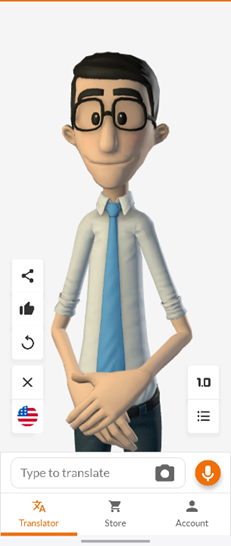
\includegraphics[width=0.25\linewidth]{figuras/handTalk.png}
    \caption{Muestra de aplicación “Hand Talk Translator”}
    \label{fig:enter-label}
\end{figure}


\paragraph{SLAIT – Real-time Sign Language Translator with AI}

Es una aplicación en fase beta que ofrece servicios de traducción de lengua de señas americanas en tiempo real para dispositivos móviles, web, entre otros. Utiliza inteligencia artificial para realizar traducciones en tiempo real, otorgando facilidad de comunicación para comunicación diaria, salud, educación y oficina. Esta aplicación tendrá modalidad de pago, aunque permite ser parte de la aplicación beta sin costo pero con previo análisis del caso por la empresa \cite{SLAIT}.

\begin{itemize}
    \item \textbf{Funcionalidades destacadas}
    \begin{itemize}
        \item Traducción instantánea de voz a texto.
        \item Traducción instantánea de señas a texto.
    \end{itemize}

    \item \textbf{Características de Diseño}
    \begin{itemize}
        \item Diseño simple y amigable con el usuario.
    \end{itemize}
\end{itemize}

\begin{figure} [H]
    \centering
    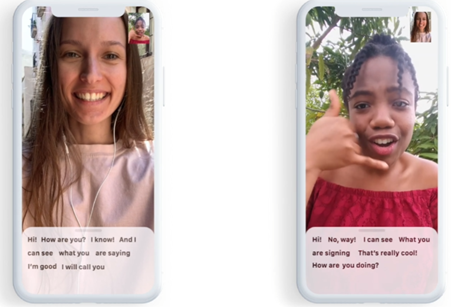
\includegraphics[width=0.5\linewidth]{figuras/slait.png}
    \caption{Muestra de aplicación “SLAIT”}
    \label{fig:enter-label}
\end{figure}

\paragraph{Lenguaje de Señas IA}

La aplicación ofrece una plataforma de traducción de señas ASL a texto y viceversa, con múltiples funciones como búsqueda por categoría, emoji y alfabeto, y soporte para diez idiomas. Con más de 2,600 señas reconocidas, busca facilitar la comunicación y el aprendizaje del lenguaje de señas \cite{LenguajeDeSeñasIA}.

\begin{itemize}
    \item \textbf{Funcionalidades destacadas}
    \begin{itemize}
        \item Grabación de señas ASL para su reconocimiento y traducción a 10 diferentes idiomas.
        \item Traducción de frases en inglés a señas ASL, seña por seña.
        \item Búsqueda de señas por emoji, categoría, palabra y alfabéticamente.
    \end{itemize}

    \item \textbf{Características de Diseño}
    \begin{itemize}
        \item Paleta de colores e iconografía básica.
        \item Diseño confuso y apretado.
    \end{itemize}
\end{itemize}

\begin{figure}[H]
    \centering
    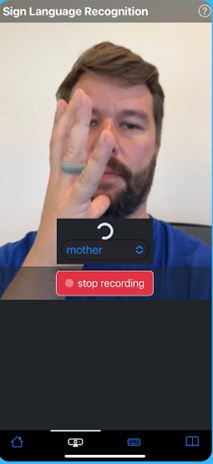
\includegraphics[width=0.2\linewidth]{figuras/applenguasenasia.png}
    \caption{Muestra de aplicación “Lenguaje de señas IA”}
    \label{fig:enter-label}
\end{figure}

\paragraph{AI Sign: Sign Language}

Es una aplicación para IOS que utiliza inteligencia artificial para reconocer más de 100 señas americanas. Tiene dos modos: reconocimiento de acciones en tiempo real y captura de datos para mejorar la precisión del modelo de aprendizaje automático \cite{AISign2023}.

\begin{itemize}
    \item \textbf{Funcionalidades destacadas}
    \begin{itemize}
        \item Capacidad de reconocimiento en tiempo real.
        \item Contiene un modo de ayuda y ajustes de configuración para personalizar la experiencia.
    \end{itemize}

    \item \textbf{Características de diseño}
    \begin{itemize}
        \item Muestra de toma de datos de las señas, señalando puntos clave de la mano.
        \item No hay paleta de colores, se usan elementos gráficos básicos.
        \item Botones poco amigables y descriptivos.
    \end{itemize}
\end{itemize}


\begin{figure} [H]
    \centering
    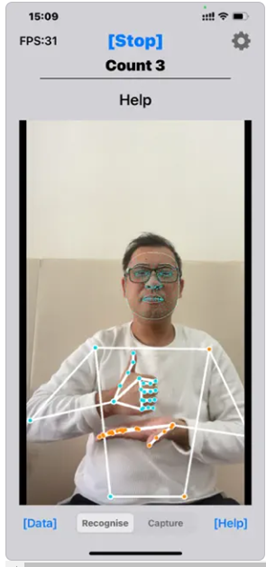
\includegraphics[width=0.25\linewidth]{figuras/ai_sign.png}
    \caption{Muestra de aplicación “AI Sign: Sign Language”}
    \label{fig:enter-label}
\end{figure}

\paragraph{Sign Language Translator AI}

Es una aplicación móvil diseñada para reconocer y traducir el lenguaje de señas coreano. Utiliza inteligencia artificial para interpretar señas en tiempo real, buscando facilitar la comunicación para las personas sordomudas. La aplicación también fomenta la participación de los usuarios para mejorar su base de datos y aumentar la precisión del reconocimiento de gestos \cite{SignLanguageTranslatorAI}.

\begin{itemize}
    \item \textbf{Funcionalidades destacadas}
    \begin{itemize}
        \item Guías visuales para el posicionamiento correcto ante la cámara, esenciales para el reconocimiento de gestos.
        \item Capacidad de reconocimiento en tiempo real.
        \item Invitación a los usuarios para contribuir con sus propios gestos, ayudando a mejorar la base de datos.
        \item Lista de palabras reconocibles que sigue expandiéndose con las contribuciones de los usuarios.
    \end{itemize}

    \item \textbf{Características de diseño}
    \begin{itemize}
        \item Botones descriptivos.
        \item Interfaz simple y clara.
        \item Diseño intuitivo.
    \end{itemize}
\end{itemize}


\begin{figure} [H]
    \centering
    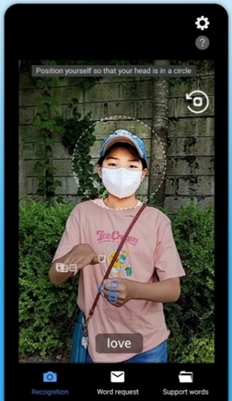
\includegraphics[width=0.25\linewidth]{figuras/ai_sign_lenguaje.png}
    \caption{Muestra de aplicación “Sign Language Translator AI”}
    \label{fig:enter-label}
\end{figure}

\paragraph{Resumen de funcionalidades y características destacadas de aplicaciones investigadas}

Luego de la investigación previa, se destacan las siguientes funcionalidades:
\begin{itemize}
    \item Espacio para grabar un video con indicadores de posición y luz adecuados para garantizar una captura óptima del vídeo.
    \item Modo ayuda para tutorial.
    \item Botón de compartir para difundir textos traducidos en redes sociales.
    \item Botón de agregar a favoritos la traducción realizada.
    \item Botón de reproducción de voz.
    \item Botón para calificar la traducción.
    \item Historial de videos grabados.
    \item Lista de palabras reconocibles.
\end{itemize}

Asimismo, destacan las siguientes características de diseño:
\begin{itemize}
    \item Diseño limpio e intuitivo.
    \item Paleta de colores atractiva.
    \item Botones descriptivos para mayor comprensión de su función.
\end{itemize}

% ---------------------------------------------------------------------------------------------------------------

\subsubsection{Investigación de la situación actual de los sordos en Guatemala}

En Guatemala, se estima que hay aproximadamente 240,000 personas sordas, lo que representa el 3\% de la población mayor de cuatro años, según datos del Instituto Nacional de Estadística (INE). Las causas de la sordera son diversas e incluyen factores genéticos, complicaciones durante el nacimiento y enfermedades infecciosas. Uno de los principales desafíos que enfrentan las personas sordas en el país es la comunicación, lo cual limita su capacidad para participar de manera equitativa en la sociedad \cite{CongresoGuatemala} \cite{GobiernoGuatemala2022}.

La lengua de señas reconocida es LENSEGUA. Las personas sordas están dispersas por todo el territorio nacional, pero se estima que la mayoría que saben LENSEGUA están concentradas principalmente en la ciudad capital. En áreas rurales con acceso limitado a la educación, como el norte de Petén, las personas sordas a menudo desarrollan sus propios sistemas de señas \cite{JoshuaProject}. 

El ámbito educativo presenta desafíos notables. A pesar de la existencia de organizaciones como la Asociación Nacional de Sordos de Guatemala, que brinda educación y otros servicios, las oportunidades educativas son escasas, especialmente en áreas rurales. Muchos estudiantes sordos deben alejarse de sus familias para acceder a opciones educativas que incluyan instrucción en lengua de señas. Un gran número de ellos ni siquiera tiene la oportunidad de acceder a una educación básica debido a la escasez de maestros capacitados en lengua de señas. Menos del 50\% recibe educación formal y las escuelas rara vez ofrecen niveles de educación secundaria. Aquellos que persiguen estudios superiores a menudo lo hacen sin la ayuda de intérpretes, lo que complica su aprendizaje y progreso académico. Esto perpetúa un ciclo de desventajas educativas y económicas, con altas tasas de desempleo y dependencia económica entre la comunidad sorda \cite{EndangeredLanguages}.

El desempleo es elevado en esta comunidad debido a las barreras comunicativas y la falta de adaptaciones adecuadas en los lugares de trabajo. La mayoría de las personas sordas vive con sus padres y están relegadas a trabajos de mano de obra básica debido a las barreras para obtener empleos mejor remunerados \cite{EndangeredLanguages}.

A pesar de estos retos, ha habido iniciativas para mejorar la inclusión de las personas sordas en Guatemala. Por ejemplo, el Benemérito Comité Pro-Ciegos y Sordos de Guatemala, en colaboración con SEGEPLAN, ha trabajado en promover la educación inclusiva y el empleo equitativo, aunque la implementación efectiva de estas políticas aún enfrenta obstáculos significativos \cite{GobiernoGuatemala2022}.

%------------------------------------------------------------------------------------------------------

\subsubsection{Preparación y realización de entrevistas y encuestas}

\paragraph{Entrevista a Doctor Miguel Angel Gonzalez Palacios}

El Dr. Gonzalez, médico general con más de 25 años de experiencia, compartió sus reflexiones sobre la importancia de mejorar la comunicación con pacientes sordos. Durante la entrevista, destacó las dificultades que enfrenta en su práctica diaria, particularmente en la correcta comprensión de los síntomas y necesidades de los pacientes sordos, lo cual es fundamental para proporcionar un diagnóstico preciso y un tratamiento efectivo.

El Dr. Gonzalez expresó su entusiasmo por la iniciativa de la aplicación \textit{Señas Chapinas}, mencionando que una herramienta de este tipo podría ser revolucionaria para la práctica médica. Resaltó el potencial de la aplicación para facilitar una comunicación fluida y precisa con pacientes sordos, reduciendo los malentendidos y aumentando la calidad del cuidado médico. 

\paragraph{Entrevista a Licenciada Claudia Barrillas}

En la entrevista con la abogada Barrillas, se abordó el contexto legal de las personas sordomudas en Guatemala, destacando la importancia de proteger sus derechos en los procedimientos judiciales. Se resaltó la necesidad de contar siempre con un intérprete de lengua de señas durante las declaraciones para asegurar una comunicación efectiva. La escasez de intérpretes, sin embargo, puede provocar demoras en los procesos legales. La Licenciada Barrillas enfatizó el valor de una aplicación de traducción de lengua de señas que podría permitir una comunicación más fluida y directa, reduciendo la dependencia de intermediarios y mejorando el acceso a la justicia para las personas sordomudas, fomentando la inclusión y la igualdad.

Se mencionaron casos donde la ausencia de intérpretes resultó en injusticias o malentendidos legales, subrayando la importancia de una comunicación clara y efectiva en el ámbito judicial. La profesional propuso que una aplicación de traducción de lengua de señas no solo facilitaría la comunicación en procesos legales, sino que también promovería una mayor autonomía para las personas sordomudas, eliminando muchas barreras que enfrentan cotidianamente.

\paragraph{Entrevista con Profesora Carmen Lucía Guerrero}

Carmen Guerrero es profesora en la Universidad del Valle de Guatemala y forma parte del departamento de Educación para personas con necesidades especiales. Su trabajo le ha permitido adquirir conocimientos en LENSEGUA y establecer contacto directo con miembros de la comunidad sorda.

En esta entrevista se abordaron temas clave sobre la estructura y adaptación del español signado en la lengua de señas. 

La profesora Guerrero explicó que las personas que nacen sordas generalmente aprenden la lengua de señas como su primer idioma, lo cual posee una gramática y estructura propias, distintas del español hablado. Por otro lado, aquellas que pierden la audición más tarde en la vida pueden intentar adaptar su forma de hablar al español, conservando características del lenguaje oral. Este contraste muestra cómo la forma de comunicación varía significativamente entre quienes han sido sordos desde el nacimiento y quienes se han vuelto sordos posteriormente.

Uno de los desafíos discutidos fue la falta de un estándar unificado en la lengua de señas en Guatemala, lo que lleva al uso de señas específicas en regiones como Quetzaltenango. Esta variabilidad regional complica la comunicación y la educación en lengua de señas. Además, la profesora subrayó la importancia de contar con intérpretes y educadores certificados por el Ministerio de Educación para asegurar utilizar LENSEGUA “oficial”. 

También se mencionó que muchas de las señas utilizadas en Guatemala son adaptaciones de la lengua francesa, compartiendo similitudes gramaticales con este idioma. La licenciada recomendó la necesidad de investigar más sobre estas reglas gramaticales y consultar documentación específica que pueda profundizar el entendimiento y la correcta aplicación de la lengua de señas.

La conversación también resaltó la relevancia de la posición y el movimiento de las manos en la comunicación a través de señas, dado que pequeñas variaciones pueden alterar significativamente el significado de las palabras. Por ejemplo, las señas para ``hola'' y ``gracias'' son muy parecidas y pueden confundirse fácilmente. 

Finalmente, se recalcó que no siempre es posible traducir todas las palabras directamente a señas, lo que destaca la complejidad de desarrollar recursos efectivos para la comunicación en lengua de señas y la importancia de adaptar continuamente las herramientas educativas y de comunicación para satisfacer las necesidades de la comunidad sorda.


\paragraph{Entrevista a intérprete de En-Señas Melany Cordero}

Melany Cordero, quien ejerce como intérprete y maestra de nivel medio en En-Señas, acompaña a profesoras al impartir clases y asiste en la resolución de dudas de los alumnos. Comenzó su formación en LENSEGUA en la academia y obtuvo su diploma que la acredita como intérprete.

Durante la entrevista, Melany expresó que la propuesta de la aplicación \textit{Señas Chapinas} le pareció tanto útil como innovadora. Sugirió agregar elementos como juegos o retos diarios, para fomentar un aprendizaje continuo y efectivo de LENSEGUA entre los usuarios. Propuso, por ejemplo, implementar un juego de memoria o un ejercicio similar a los utilizados en exámenes, donde se presenta una palabra y los usuarios deben seleccionar la seña correcta asociada. Estas actividades no solo mantendrían el interés de los usuarios, sino que también potenciarían su capacidad de aprendizaje y retención de la lengua de señas de manera divertida y desafiante.


\paragraph{Entrevista a Director General de En-Señas Antonio Barrientos}

El señor Barrientos desarrolló un interés por la lengua de señas inspirado por su madre, quien también la aprendió y frecuentaba a la comunidad sorda. Motivado por su deseo de entender las conversaciones de este grupo, el señor se sumergió en el estudio de la lengua de señas y actualmente es intérprete de nivel avanzado y director general de la institución ``En-Señas''.

Durante la entrevista, el Director señaló que una de las principales complicaciones con la aplicación \textit{Señas Chapinas} es la falta de un estándar uniforme para LENSEGUA. Explicó que existen variaciones significativas en el uso de señas entre los diferentes departamentos de Guatemala, e incluso entre distintas instituciones educativas, lo que puede complicar la precisión de las traducciones. Esta diversidad se debe a la ausencia de una entidad reguladora que estandarice las señas y certifique quiénes están calificados para enseñar LENSEGUA. No obstante, actualmente hay esfuerzos para lograr esta estandarización.

El Director también destacó la escasez de materiales e información en línea sobre LENSEGUA, así como las deficiencias legislativas que, aunque reconocen la lengua de señas, no establecen un marco regulatorio suficiente para su enseñanza y promoción.

En cuanto a la comunidad sorda, mencionó que existen cuatro categorías distintas: personas que utilizan señas caseras y no interactúan con LENSEGUA, aquellas que aprenden a leer los labios, los usuarios de LENSEGUA, y los bilingües, que combinan la lectura de labios con el uso de la lengua de señas.

Finalmente, el Director Barrientos abordó el alto índice de analfabetismo en la comunidad sorda, atribuyéndolo a las diferencias en el nivel de apoyo que reciben desde la infancia. Mientras algunas familias fomentan el aprendizaje de la lengua de señas y la terapia del habla desde temprana edad, otras dejan a las personas sordas sin el soporte necesario para su desarrollo educativo.

\paragraph{Entrevista a persona sorda hipoacúsica y maestra de En-Señas Gabriela Velázquez}
La señora Velázquez, una maestra de 59 años de En-Señas y persona sorda hipoacúsica, nació en Guatemala y actualmente enseña LENSEGUA tanto a personas sordas como oyentes. Está casada con una persona sorda profunda. 

Durante su infancia, la señora Gabriela relata que era común que las personas sordas fueran obligadas a aprender a vocalizar mediante terapia del habla y lectura de labios, en lugar de aprender LENSEGUA. No fue hasta la edad adulta que aprendió este medio de comuniación, convirtiéndose en bilingüe, lo cual marcó una mejora significativa en su comprensión lectora y en la ampliación de su vocabulario. Aunque la profesora puede leer labios, encuentra este método desafiante y prefiere comunicarse usando LENSEGUA, lo que le resulta más cómodo y eficaz. Ella señala que, para las personas sordas profundas, vocalizar puede ser aún más difícil, por lo que generalmente dependen más de LENSEGUA, lo que a menudo complica su comprensión del español escrito.

Sobre la aplicación \textit{Señas Chapinas}, la profesora Gabriela considera que sería útil para usuarios de LENSEGUA y destacó la importancia de que la aplicación ofrezca tanto la traducción palabra por palabra como la oración completa en español. Esto ayudaría a los usuarios a verificar la traducción de las señas y facilitaría el aprendizaje de la gramática en español. La profesora Velázquez y sus conocidos frecuentemente utilizan \textit{ChatGPT}, escribiendo en gramática de LENSEGUA para que el sistema lo traduzca al español, lo que les ayuda a confirmar que están escribiendo correctamente.

Ella menciona que \textit{Señas Chapinas} la usaría principalmente en situaciones donde no hay un intérprete presente, como visitas al médico, reuniones con abogados, testimonios en corte, emergencias y reuniones familiares. Menciona que en Estados Unidos existe un servicio de intérpretes que funciona como un \textit{call center}, donde se ofrece traducción a lengua de señas de forma simultanea, y sugiere que la aplicación podría replicar este servicio en Guatemala, ofreciendo traducciones de LENSEGUA a texto o voz.

Además, destacó que la aplicación podría contribuir a reducir el analfabetismo entre los sordos, permitiéndoles aprender al grabar videos en LENSEGUA y ver las traducciones al español. 

En el contexto de las aplicaciones móviles, se destacó que las personas sordas utilizan continuamente sus teléfonos, especialmente para acceder a redes sociales y aplicaciones de videollamadas. Estas herramientas les permiten interactuar con amigos, familiares y conocidos de manera más dinámica. Continua relatando que antes de la llegada de los teléfonos inteligentes, la comunicación era notablemente más complicada; sin embargo, hoy en día, la tecnología facilita significativamente el aprendizaje de LENSEGUA en línea y mejora la comunicación general. 

La profesora Velázquez prefiere las aplicaciones que requieren poco texto y presentan interfaces de usuario simples y directas, ya que son más fáciles de utilizar. Además, comentó que las aplicaciones lentas y complejas resultan menos atractivas para los ella y sus conocidos.

Para la profesora, un aspecto crucial de la aplicación \textit{Señas Chapinas} es que reconozca las diversas variantes y modismos presentes en LENSEGUA. Este detalle es fundamental para asegurar que la aplicación sea verdaderamente inclusiva y efectiva para todos los usuarios de la lengua de señas guatemalteca, reflejando las diferencias regionales y de estilo que caracterizan su uso cotidiano.

Además, Gabriela Velázquez espera que la aplicación le sirva como una herramienta para enriquecer su vocabulario y gramática en español. Al incorporar funciones que permitan aprender y practicar español, la aplicación no solo serviría para traducir de LENSEGUA a español, sino que también funcionaría como un recurso educativo, apoyando el desarrollo lingüístico integral de sus usuarios.


\begin{figure} [H]
    \centering
    \includegraphics[width=0.5\linewidth]{figuras/entrevista.png}
    \caption{Entrevista En-Señas}
    \label{fig:enter-label}
\end{figure}

\paragraph{Primera encuesta Señas Chapinas}

La primera encuesta para el proyecto \textit{Señas Chapinas} consta de varias secciones diseñadas para recopilar información y opiniones sobre la necesidad de superar las barreras de comunicación en Guatemala a través de una aplicación móvil.

La primera sección recopila datos demográficos como edad, género, lugar de nacimiento, profesión y si el encuestado presenta dificultades auditivas o del habla.

La segunda sección está bifurcada según si los encuestados son sordos o no. Para los que no son sordos, se investiga si conocen a alguien con dificultades auditivas y cómo han utilizado tecnología de asistencia para comunicarse con ellos. Además, se indaga sobre los desafíos percibidos para estas personas y en qué contextos una aplicación de traducción de señas sería beneficiosa. Para los encuestados sordos, se solicita que compartan sus experiencias con otras herramientas de asistencia, desafíos específicos enfrentados en Guatemala, situaciones de frustración al comunicarse, y cómo una aplicación podría mejorar su comunicación diaria.

La tercera sección evalúa la percepción sobre la utilidad de la aplicación para convertir la lengua de señas a texto o voz, recogiendo expectativas y características deseadas. Además, se piden sugerencias sobre funcionalidades adicionales y posibles contextos de uso.

Los resultados de esta primera encuesta no fueron los esperados. Los participantes sordos de nacimiento encontraron las preguntas demasiado complejas, atribuyéndolo a las diferencias gramaticales en su lenguaje. Esto llevó a la necesidad de desarrollar una encuesta específica para personas oyentes y planificar entrevistas con intérpretes para personas sordas.


\paragraph{Segunda encuesta Señas Chapinas}

Como resultado de los comentarios y sugerencias recopilados en la primera encuesta, se desarrolló una segunda encuesta dirigida específicamente a personas oyentes (ver Anexo~\ref{anexo:encuesta_oyentes}). Esta encuesta se dirige a individuos sin conocimiento previo de LENSEGUA, a aquellos que regularmente interactúan con personas sordas, y a intérpretes. 

La sección inicial de la encuesta proporciona un análisis demográfico de los participantes. Los resultados muestran que la mayoría de los encuestados son hombres. Además, el grupo de edad más representado está entre los 18 y 24 años. 

\begin{figure} [H]
    \centering
    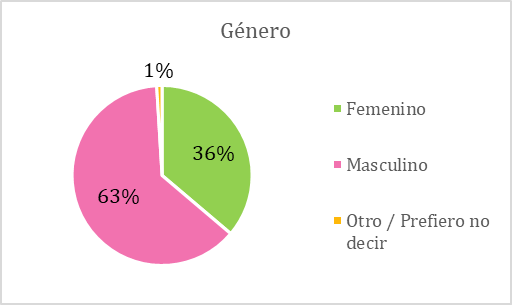
\includegraphics[width=0.5\linewidth]{figuras/encuesta_genero.png}
    \caption{Género Encuesta 2}
    \label{fig:enter-label}
\end{figure}

\begin{figure} [H]
    \centering
    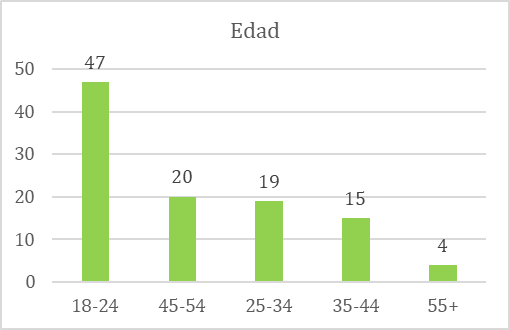
\includegraphics[width=0.5\linewidth]{figuras/encuesta_edad.png}
    \caption{Edad Encuesta 2}
    \label{fig:enter-label}
\end{figure}

La siguiente sección de la encuesta está destinada a explorar el conocimiento y la experiencia con la lengua de señas. Alrededor del 40\% de los encuestados indica conocer a alguien sordo, lo que destaca una conexión significativa con la comunidad sorda. Adicionalmente, cerca del 70\% percibe la aplicación como relevante, mostrando un interés considerable en la herramienta propuesta. Sin embargo, es notable que aproximadamente el 70\% de los participantes no están familiarizados con LENSEGUA, lo cual es entendible considerando que su reconocimiento oficial data de hace solo cuatro años. \cite{CongresoGuatemala2020}. 

\begin{figure} [H]
    \centering
    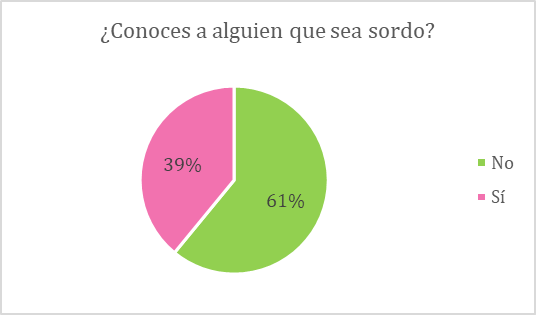
\includegraphics[width=0.5\linewidth]{figuras/conocimientoSordaEncuesta.png}
    \caption{Conocimiento Persona Sorda Encuesta 2}
    \label{fig:enter-label}
\end{figure}

\begin{figure} [H]
    \centering
    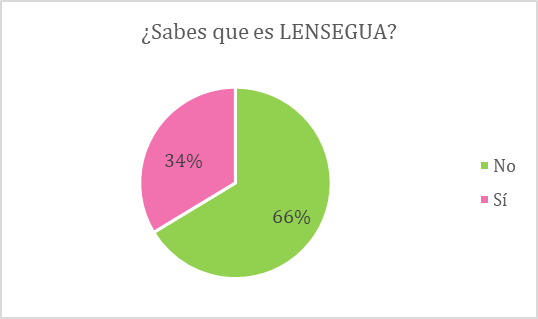
\includegraphics[width=0.5\linewidth]
    {figuras/conoimiento_lensegua.png}
    \caption{Conocimiento LENSEGUA Encuesta 2}

\end{figure}

\begin{figure} [H]
    \centering
    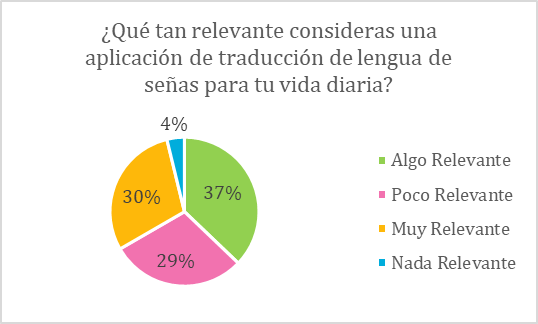
\includegraphics[width=0.5\linewidth]{figuras/relevancia_app.png}
    \caption{ Relevancia de la Aplicación Encuesta 2}
    \label{fig:enter-label}
\end{figure}


Además, se realizó un análisis comparativo entre los encuestados que conocen a personas sordas y su percepción de la relevancia de la aplicación. Los resultados muestran que aquellos familiarizados con la comunidad sorda tienden a valorar más la aplicación en comparación con quienes no tienen contacto directo con personas sordas. Este hallazgo sugiere que la experiencia personal y el conocimiento de los retos enfrentados por las personas sordas pueden influir significativamente en la percepción de la utilidad de herramientas tecnológicas como un traductor de lengua de señas.

\begin{figure} [H]
    \centering
    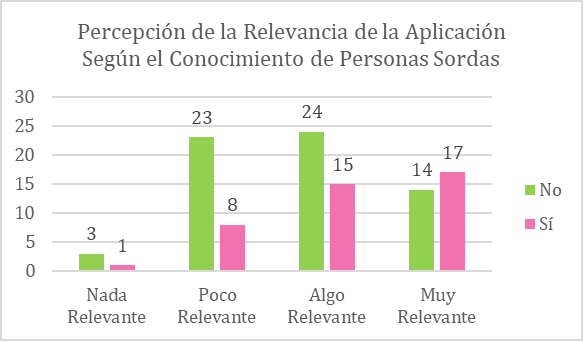
\includegraphics[width=0.5\linewidth]{figuras/relevancia_app_conocidos.png}
    \caption{Relevancia de la Aplicación para Personas con Conocidos Sordos Encuesta 2}
    \label{fig:enter-label}
\end{figure}

Para comprender mejor las estrategias de comunicación que las personas emplearían con individuos sordos, se les preguntó a los encuestados sobre sus métodos preferidos. La mayoría, casi el 60\%, optaría por el uso de mensajes escritos, mientras que un 18\% indicó que señalarían objetos para hacerse entender. Solo un 9\% consideraría usar LENSEGUA. Es notable que solo una minoría, aproximadamente el 10\%, expresó no saber cómo comunicarse, reflejando así el interés general por explorar formas de interacción. Algunos participantes también mencionaron la lectura de labios como alternativa, aunque es importante destacar que no todos los sordos tienen la capacidad de leer los labios.

Para profundizar en el entendimiento que tienen las personas sobre los desafíos que enfrentan los sordos, se les preguntó cuáles consideraban que eran las mayores dificultades para esta comunidad. Las respuestas revelaron una conciencia sobre la falta de inclusión y herramientas adecuadas para personas sordas, destacando cómo muchas infraestructuras y servicios en Guatemala están diseñados principalmente para oyentes. Además, se mencionaron problemas como segregación y discriminación en la sociedad, así como la escasez de enseñanza de la lengua de señas.

Entre las preocupaciones más citadas también estuvieron la ausencia de sistemas de alerta para sordos en situaciones de emergencia y barreras significativas en comunicación. Los encuestados resaltaron la existencia de prejuicios y la dificultad en la realización de tareas cotidianas y trámites, lo que contribuye al aislamiento social y a la exclusión. Esta variedad de respuestas ilustra la complejidad de los desafíos a los que se enfrentan los sordos. 

La siguiente sección de la encuesta se centró en la aplicación \textit{Señas Chapinas}, explorando las motivaciones principales para usar una herramienta de traducción de lengua de señas. Destacablemente, el 60\% de los participantes indicaron la curiosidad personal como su principal motivación. Casi la mitad de los encuestados mencionaron la comunicación con amigos o familiares sordos como un factor importante, subrayando la relevancia personal y social de la aplicación. Además, cerca del 40\% expresaron que utilizarían la aplicación para actividades voluntarias, lo que refleja su potencial utilidad en entornos de servicio comunitario. Un pequeño porcentaje citó los requerimientos laborales como motivo, sugiriendo su aplicación en contextos profesionales donde la interacción con personas sordas es frecuente. Otras respuestas revelaron usos más específicos y personales, evidenciando la diversidad de situaciones en las que los usuarios anticipan la utilidad de la aplicación.

También se indagó en que situaciones los usuarios desean emplear la aplicación \textit{Señas Chapinas}. Predominantemente, las actividades sociales representan el escenario más popular, con un 78.6\% de los encuestados seleccionándolo. Esto es seguido por el voluntariado y la educación, con un 67.6\% y un 49\%, respectivamente. El trabajo también es una situación comúnmente identificada, con un 40.2\% de los encuestados expresando la necesidad de utilizar la aplicación en este contexto. Estos resultados indican una fuerte preferencia por utilizar la aplicación en contextos grupales y de interacción, lo que subraya la importancia de la aplicación en facilitar la comunicación en una variedad de entornos cotidianos y profesionales.

La última sección pregunta las características más importantes en una aplicación móvil. En la última sección de la encuesta, los encuestados identificaron las características más importantes en una aplicación móvil. La facilidad de uso fue la más destacada, valorada por el 98.1\% de los participantes, seguida por la velocidad y rendimiento (61.9\%), funciones de accesibilidad (54.3\%), y diseño atractivo (46.7\%). Esto resalta la importancia de una interfaz intuitiva, un rendimiento eficiente, accesibilidad adecuada, y un diseño visualmente atractivo para los usuarios de esta aplicación. 

Finalmente se dio espacio para comentarios adicionales. En la sección final de la encuesta se exploraron las características esenciales para una aplicación de traducción de lengua de señas. La facilidad de uso fue una de las características más mencionadas, destacando su importancia para una adopción rápida por parte de los usuarios. Muchos encuestados valoraron también la velocidad y la precisión de la traducción, subrayando la necesidad de interacciones fluidas y sin errores. Algunas otras sugerencias fueron mencionadas, pero serán tomadas en cuenta para futuras mejoras, pues no están dentro del alcance del presente proyecto. 

\paragraph{Entrevista colectiva a miembros de En-Señas}

Con un conocimiento más profundo de las necesidades de las personas sordas, sus familias y conocidos, así como del nivel de conciencia de la población guatemalteca sobre LENSEGUA, se llevó a cabo una última entrevista colectiva con miembros de Enseñas. Durante esta sesión, se presentó el concepto de la aplicación y se recogieron sus opiniones. Los comentarios más destacados incluyeron:

\begin{itemize}
    \item \textbf{Uso de Redes Sociales:} Las personas sordas frecuentan plataformas sociales, especialmente TikTok, por su facilidad e intuitividad de uso.
    
    \item \textbf{Funcionalidades Educativas}: Se sugirió que la aplicación también debería facilitar el aprendizaje de LENSEGUA en Guatemala, incorporando juegos interactivos que fomenten la participación activa.
    
    \item \textbf{Diseño Atractivo y Profesional}: La aplicación debe ser visualmente llamativa sin sacrificar su seriedad, generando confianza en que se trata de una herramienta fiable y efectiva.
    
    \item \textbf{Futuras Expansiones}: Se anticipa que, eventualmente, la aplicación podrá traducir del español a LENSEGUA.
    
    \item \textbf{Vocabulario Adecuado}: En las primeras fases, el vocabulario debe ser simple y cotidiano, incluyendo términos de uso frecuente y frases de emergencia.
    
    \item \textbf{Reporte de Errores:} Es crucial que las traducciones incorrectas puedan ser reportadas fácilmente por los usuarios sordos para que el equipo detrás de la aplicación pueda investigar y resolver cualquier inconveniente.
    
    \item \textbf{Guardado de Favoritos:} Los usuarios expresaron el deseo de poder guardar videos de frases en LENSEGUA que utilizan regularmente, para acceder a ellos de manera rápida y sencilla.
    
    \item \textbf{Flexibilidad de Grabación}: La aplicación debe permitir grabaciones tanto con la cámara frontal como con la trasera, facilitando la captura de auto-grabaciones o de terceros.
    
    \item \textbf{Accesibilidad del Nombre}: El nombre de la aplicación debe ser fácilmente representable en señas, asegurando su accesibilidad y reconocimiento dentro de la comunidad sorda.
    
\end{itemize}

Estos valiosos comentarios guiaran la próxima fase de desarrollo para asegurar que la aplicación no solo cumpla con las expectativas de la comunidad sorda sino que también sirva como un puente cultural y educativo.


\begin{figure} [H]
    \centering
    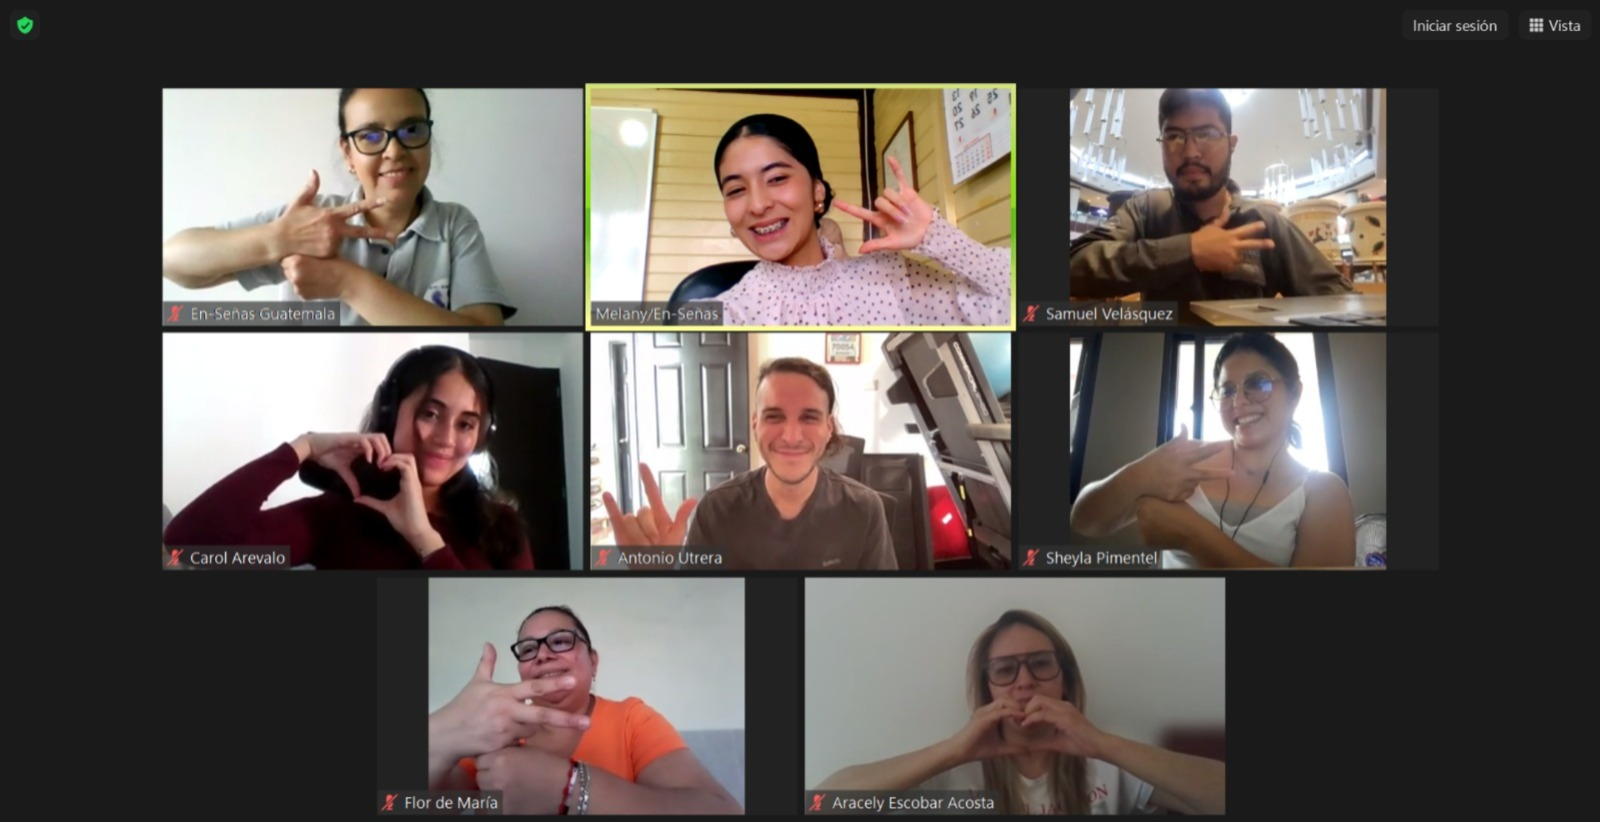
\includegraphics[width=0.75\linewidth]{figuras/entrevista_colectiva.png}
    \caption{Entrevista colectiva En-Señas}
    \label{fig:enter-label}
\end{figure}


%-------------------------------------------------------------------------------------------------------------------------------

\subsubsection{Colaboraciones}

Para profundizar en la comprensión de las necesidades tanto de las personas sordas como de aquellas que desean comunicarse con ellas, se decidió colaborar con varias entidades guatemaltecas dedicadas a mejorar la calidad de vida de este grupo.

En primer lugar, se participó en clases de Lengua de Señas Guatemalteca (LENSEGUA) ofrecidas por En-Señas. Esta formación permitió comprender mejor la gramática y el contexto cultural de esta lengua, elementos fundamentales para garantizar una comunicación efectiva y respetuosa.

Asimismo, la empresa ASEDES colaboró proporcionando apoyo en la realización de entrevistas y en otras actividades necesarias para el desarrollo de los diversos módulos del proyecto. Esta colaboración fue vital para asegurar que el diseño de la aplicación sea inclusivo y práctico para los usuarios.

Finalmente, la ONG Sordos Latinos de Guatemala estuvo brindando asistencia invaluable mediante el suministro de información y recomendaciones especializadas. Además, facilito entrevistas y otros recursos esenciales que enriquecieron el entendimiento y ayudaron a ajustar el proyecto para entender mejor las necesidades de la comunidad sorda en Guatemala.

%======================================================================================================
\subsection{Desarrollo de interfaz y experiencia de usuario}

\subsubsection{Creación de diagrama de afinidad}

En el desarrollo de la experiencia del usuario (UX), los diagramas de afinidad juegan un papel crucial, ya que permiten organizar y sintetizar grandes volúmenes de datos e ideas de manera visual y estructurada. Este método es especialmente valioso durante las fases iniciales de desarrollo de un proyecto, donde el entendimiento claro y la definición del problema son esenciales \cite{Maze2024}.

El proceso comienza con una lluvia de ideas, donde se generan y recopilan múltiples puntos de vista y datos sobre las necesidades y problemas de los usuarios. Esta fase es crítica, ya que establece la base de información que influirá en todas las decisiones de diseño y desarrollo subsiguientes \cite{Maze2024}.

La lluvia de ideas para Señas Chapinas organiza conceptos clave en categorías codificadas por colores, facilitando la identificación y el análisis de diversas áreas del proyecto:

\begin{itemize}
    \item \textbf{Naranja:} Define el público objetivo de la aplicación.
    \item \textbf{Amarillo:} Enumera los objetivos y metas que la aplicación pretende alcanzar.
    \item \textbf{Azul:} Destaca información crucial necesaria para el desarrollo de la aplicación.
    \item \textbf{Rojo:} Señala los problemas y desafíos que la aplicación busca resolver.
    \item \textbf{Verde:} Detalla las características y funcionalidades esperadas de la aplicación.
\end{itemize}

Este enfoque visual no solo ayuda a estructurar el proceso de planificación, sino que también asegura que todos los aspectos relevantes sean considerados, apoyando una toma de decisiones informada y alineada con las necesidades de los usuarios.

\begin{figure} [H]
    \centering
    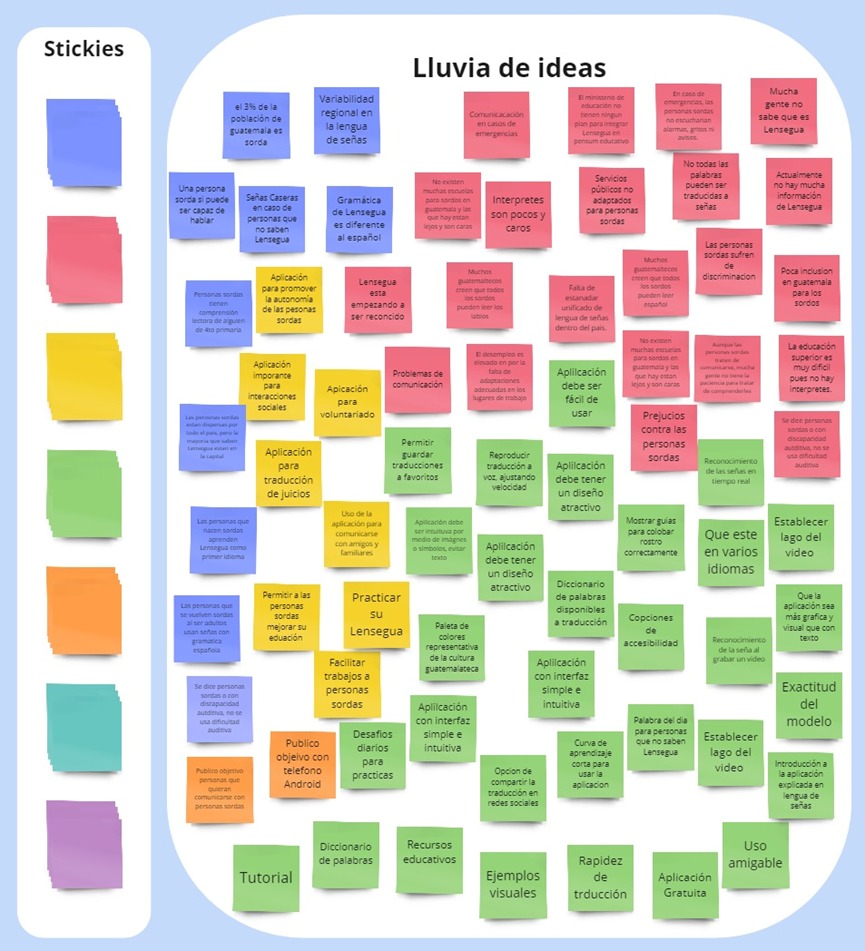
\includegraphics[width=0.75\linewidth]{figuras/lluevia_diagrama_afinidad.png}
    \caption{Lluvia de Ideas para Diagrama de Afinidad}
    \label{fig:enter-label}
\end{figure}

Posteriormente, se agrupan las ideas similares con el objetivo de identificar patrones y temas comunes. Este proceso implica organizar los datos recolectados durante la lluvia de ideas en categorías que reflejen conexiones y tendencias subyacentes. Al hacer esto, se pueden observar relaciones entre las diferentes opiniones y necesidades, facilitando la creación de soluciones más coherentes y efectivas que aborden los desafíos identificados de manera integral. Este método no solo ayuda a clarificar el alcance del proyecto, sino que también proporciona una base sólida para las decisiones de diseño y desarrollo subsiguientes, asegurando que se consideren todas las perspectivas relevantes.

\begin{figure} [H]
    \centering
    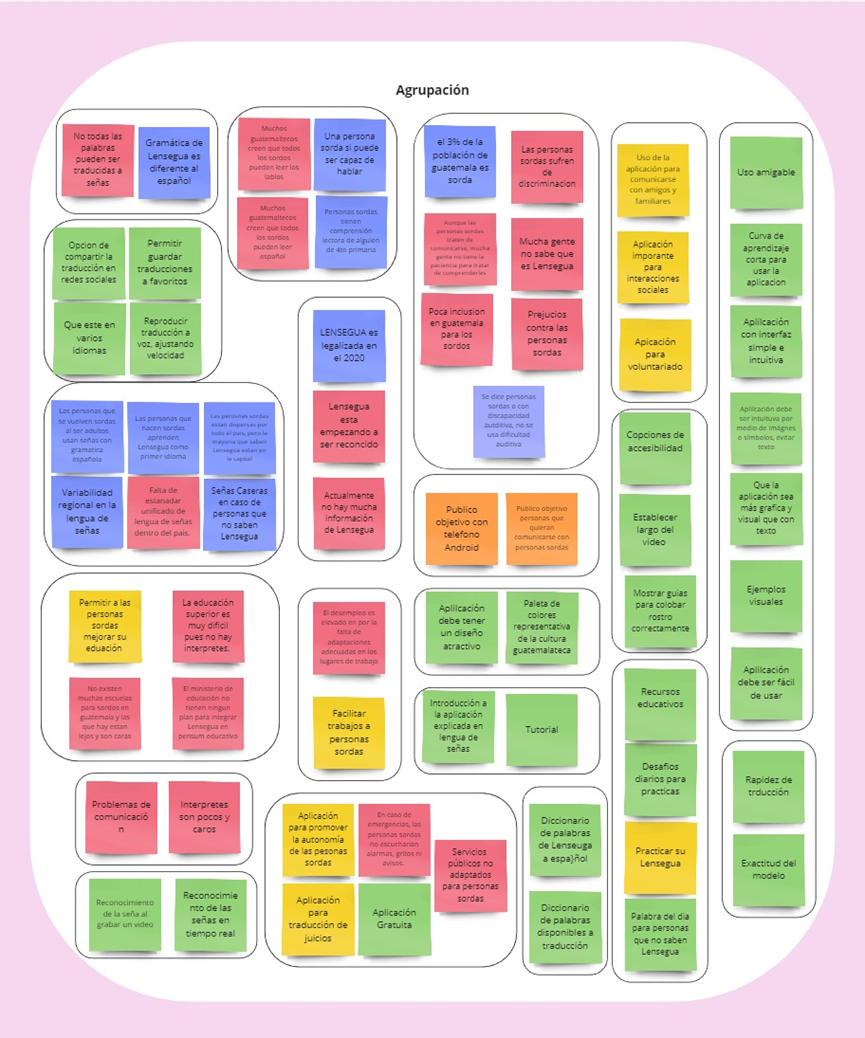
\includegraphics[width=0.75\linewidth]{figuras/agrupacion_diagrama_afinidad.png}
    \caption{Agrupación de Ideas para Diagrama de Afinidad}
    \label{fig:enter-label}
\end{figure}

Finalmente, se realiza el diagrama de afinidad, que sintetiza todas las ideas recolectadas y categorizadas previamente. Este diagrama visual, organizado por colores, facilita la interpretación de la información y permite una evaluación clara de cómo cada aspecto del proyecto interacciona y contribuye al objetivo global. Al agrupar las ideas en distintas categorías, como Público Objetivo, Problemas a Resolver, Objetivos, Escenarios de Uso, Funcionalidades a Desarrollar y Características de la Aplicación, se destaca la interconexión entre los requisitos del usuario y las soluciones propuestas.

\begin{figure} [H]
    \centering
    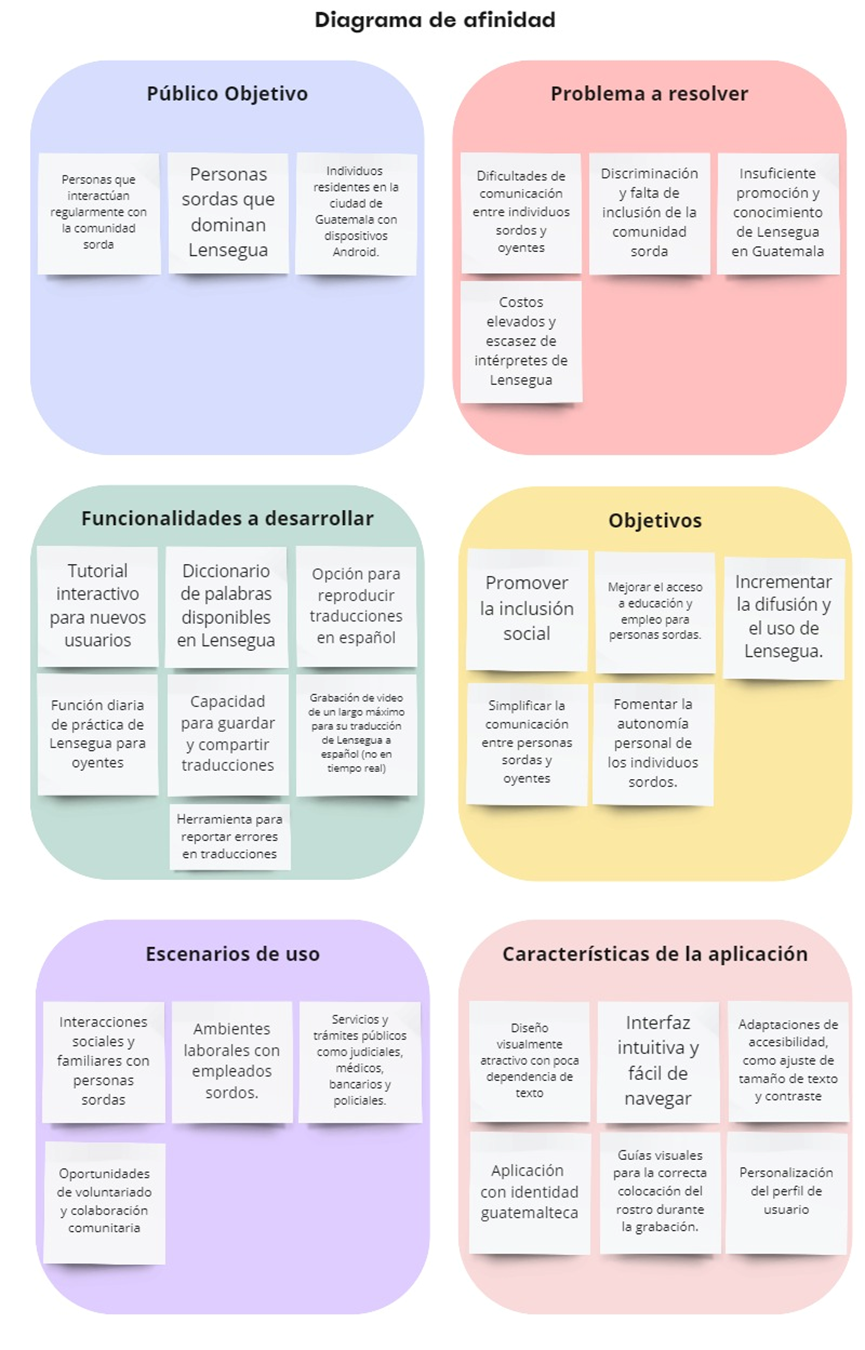
\includegraphics[width=1\linewidth]{figuras/diagrama_afinidad.png}
    \caption{Diagrama de Afinidad}
    \label{fig:enter-label}
\end{figure}

\begin{enumerate}

    \item \textbf{Público Objetivo} 
    Define a las personas que se beneficiarán directamente de la aplicación, incluyendo a aquellos que interactúan regularmente con la comunidad sorda y a las personas sordas que dominan LENSEGUA.
    \begin{itemize}
        \item Personas que interactúan regularmente con la comunidad sorda
        \item Personas sordas que dominan LENSEGUA
        \item Individuos residentes en la ciudad de Guatemala con dispositivos Android
    \end{itemize}
    
    \item \textbf{Problema a Resolver} 
    Identifica los principales desafíos que enfrenta la comunidad sorda y que la aplicación busca abordar, como las dificultades de comunicación entre sordos y oyentes, la discriminación y los altos costos de los servicios de interpretación.
    \begin{itemize}
        \item Dificultades de comunicación entre individuos sordos y oyentes
        \item Discriminación y falta de inclusión de la comunidad sorda
        \item Costos elevados y escasez de intérpretes de LENSEGUA
    \end{itemize}
    
    \item \textbf{Funcionalidades a Desarrollar} 
    Describe las características específicas que tendrá la aplicación. 
    \begin{itemize}
        \item Diccionario de palabras disponibles en LENSEGUA
        \item Función diaria de práctica de LENSEGUA para oyentes
        \item Capacidad para guardar y compartir traducciones
        \item Herramienta para reportar errores en traducciones
        \item Opción para reproducir traducciones en español
        \item Grabación de video de un largo máximo para su traducción de LENSEGUA a español (no en tiempo real)
    \end{itemize}
    
    \item \textbf{Objetivos} 
    Detalla los objetivos principales de la aplicación, como promover la inclusión social, mejorar el acceso a la educación y empleo para personas sordas, y simplificar la comunicación entre sordos y oyentes.
    \begin{itemize}
        \item Promover la inclusión social
        \item Simplificar la comunicación entre personas sordas y oyentes
        \item Mejorar el acceso a educación y empleo para personas sordas
        \item Fomentar la autonomía personal de los individuos sordos
        \item Incrementar la difusión y el uso de LENSEGUA
    \end{itemize}
    
    \item \textbf{Escenarios de Uso} 
    Enumera los diferentes contextos en los que la aplicación podría ser utilizada, incluyendo interacciones sociales, ambientes laborales, y servicios públicos como trámites médicos, bancarios y policiales.
    \begin{itemize}
        \item Interacciones sociales y familiares con personas sordas
        \item Ambientes laborales con empleados sordos
        \item Servicios y trámites públicos como judiciales, médicos, bancarios y policiales
        \item Oportunidades de voluntariado y colaboración comunitaria
    \end{itemize}
    
    \item \textbf{Características de la Aplicación} 
    Resalta aspectos del diseño y la usabilidad de la aplicación, tales como su interfaz intuitiva, el diseño visual con poca dependencia de texto y adaptaciones para accesibilidad, entre otros.
    \begin{itemize}
        \item Diseño visualmente atractivo con poca dependencia de texto
        \item Interfaz intuitiva y fácil de navegar
        \item Aplicación con identidad guatemalteca
        \item Guías visuales para la correcta colocación del rostro durante la grabación
        \item Personalización del perfil de usuario
    \end{itemize}
\end{enumerate}


\subsubsection{Creación de personas}

Como parte del proceso de diseño, se han definido seis personas que representan a los usuarios finales a quienes se dirige la aplicación. 

\begin{figure} [H]
    \centering
    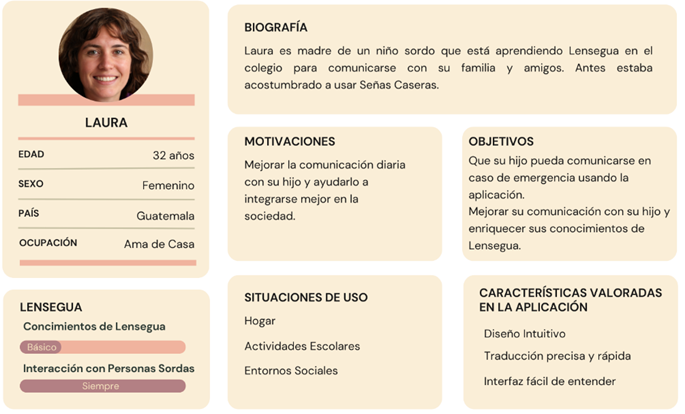
\includegraphics[width=0.8\linewidth]{figuras/persona_laura.png}
    \caption{Persona 1 - Laura}
    \label{fig:enter-label}
\end{figure}

\begin{figure} [H]
    \centering
    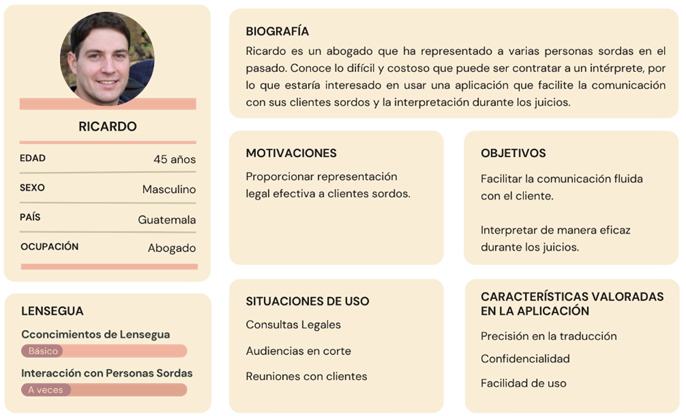
\includegraphics[width=0.8\linewidth]{figuras/ricardo_persona.png}
    \caption{Persona 2 - Ricardo}
    \label{fig:enter-label}
\end{figure}

\begin{figure} [H]
    \centering
    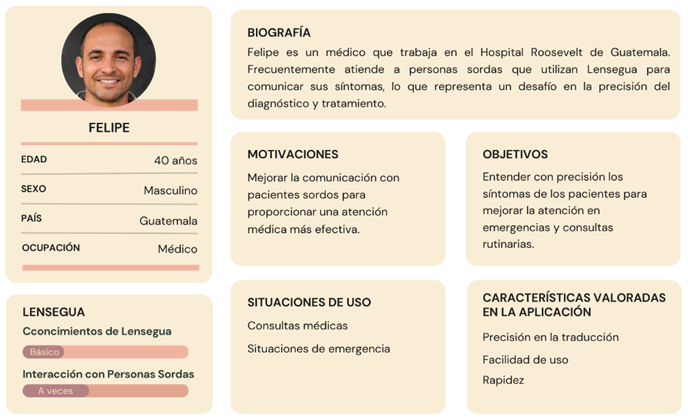
\includegraphics[width=0.8\linewidth]{figuras/felipe_persona.png}
    \caption{Persona 3 - Felipe}
    \label{fig:enter-label}
\end{figure}

\begin{figure} [H]
    \centering
    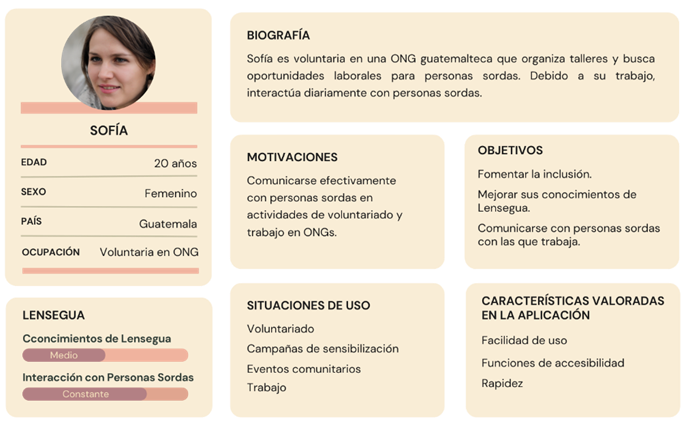
\includegraphics[width=0.8\linewidth]{figuras/sofia_persona.png}
    \caption{Persona 4 - Sofia}
    \label{fig:enter-label}
\end{figure}

\begin{figure}[H]
    \centering
    \includegraphics[width=0.8\linewidth]{figuras/marta_persona.png}
    \caption{Persona 5 - Marta}
    \label{fig:enter-label}
\end{figure}

\begin{figure} [H]
    \centering
    \includegraphics[width=0.8\linewidth]{figuras/jorge_persona.png}
    \caption{Persona 6 - Jorge}
    \label{fig:enter-label}
\end{figure}

% -----------------------------------------------------------------------------------------


\subsubsection{Creación de mapas de empatía}

Complementando las Personas creadas con anterioridad, se procede a crear su Mapa de Empatía respectivo para profundizar en las necesidades de los usuarios. 

\begin{figure} [H]
    \centering
    \includegraphics[width=0.9\linewidth]{figuras/mapa_empatia_laura.png}
    \caption{Mapa de Empatía - Laura}
    \label{fig:enter-label}
\end{figure}

\begin{figure} [H]
    \centering
    \includegraphics[width=0.9\linewidth]{figuras/mapa_empatia_ricardo.png}
    \caption{Mapa de Empatía - Ricado}
    \label{fig:enter-label}
\end{figure}

\begin{figure} [H]
    \centering
    \includegraphics[width=0.9\linewidth]{figuras/mapa_empatia_felipe.png}
    \caption{Mapa de Empatía - Felipe}
    \label{fig:enter-label}
\end{figure}

\begin{figure} [H]
    \centering
    \includegraphics[width=0.9\linewidth]{figuras/mapa_empatia_sofia.png}
    \caption{Mapa de Empatía - Sofia}
    \label{fig:enter-label}
\end{figure}


\begin{figure} [H]
    \centering
    \includegraphics[width=0.9\linewidth]{figuras/mapa_empatia_marta.png}
    \caption{Mapa de Empatía - Marta}
    \label{fig:enter-label}
\end{figure}


\begin{figure} [H]
    \centering
    \includegraphics[width=0.9\linewidth]{figuras/mapa_empatia_jorge_correcto.png}
    \caption{Mapa de Empatía - Jorge}
    \label{fig:enter-label}
\end{figure}
% -----------------------------------------------------------------------------------------

\subsubsection{Planteamiento del problema}

Inicialmente se usa Los Seis Sombreros Para Pensar, una técnica de pensamiento desarrollada por Edward de Bono en los años 80, que busca facilitar de manera creativa la resolución y el análisis de problemas desde distintos puntos de vista o perspectivas. Cada ``sombrero'' representa una dirección diferente del pensamiento y se identifica con un color específico \cite{Santos2024}.

\begin{figure} [H]
    \centering
    \includegraphics[width=0.8\linewidth]{figuras/sombreros.png}
    \caption{Sombreros para Pensar}
    \label{fig:enter-label}
\end{figure}


Posteriormente, se sigue el modelo W5H1 para realizar el planteamiento del problema, el cual busca ver las ideas desde varias perspectivas con el objetivo de comprender en profundidad una situación concreta \cite{Artigas2017}.

\begin{figure} [H]
    \centering
    \includegraphics[width=0.6\linewidth]{figuras/w5h1.png}
    \caption{Planteamiento del Problema Señas Chapinas}
    \label{fig:enter-label}
\end{figure}

\begin{enumerate}
    \item \textbf{¿Quién?}
    \begin{enumerate}
        \item \textbf{¿A quién afecta el problema?} \\
        Afecta principalmente a personas sordas que utilizan la Lengua de Señas Guatemalteca (LENSEGUA), quienes enfrentan barreras de comunicación cotidianas.
        \item \textbf{¿Quiénes son los usuarios primarios y secundarios?}
        \begin{itemize}
            \item \textbf{Usuarios primarios:} Personas sordas, quienes dependen directamente de la comunicación efectiva para su inclusión social y profesional.
            \item \textbf{Usuarios secundarios:} Familiares, amigos, intérpretes de LENSEGUA, y personal de servicios públicos y privados que interactúan regularmente con personas sordas.
        \end{itemize}
    \end{enumerate}

    \item \textbf{¿Qué?}
    \begin{enumerate}
        \item \textbf{¿Cuáles son los límites del problema?} \\
        El problema está limitado al vocabulario esencial y de emergencia necesario para la comunicación diaria y situaciones críticas.
        \item \textbf{¿Cuál es el problema que requiere nuestra atención?} \\
        La barrera de comunicación persistente entre las personas sordas y la sociedad oyente, que limita significativamente la participación de las personas sordas en la sociedad.
        \item \textbf{¿Cuál es el objetivo final?} \\
        Facilitar la comunicación y mejorar la inclusión de la comunidad sorda en todos los aspectos de la vida social y profesional.
    \end{enumerate}

    \item \textbf{¿Cuándo?}
    \begin{enumerate}
        \item \textbf{¿Cuándo ocurre el problema?} \\
        El problema ocurre diariamente y se manifiesta en interacciones rutinarias, servicios de emergencia, entornos educativos y actividades sociales.
    \end{enumerate}

    \item \textbf{¿Dónde?}
    \begin{enumerate}
        \item \textbf{¿Dónde ocurre el problema?} \\
        El problema ocurre a lo largo de Guatemala, con un enfoque inicial en el departamento de Guatemala, debido a las variaciones dialectales de LENSEGUA en diferentes regiones.
        \item \textbf{¿Dónde se necesita enfocar más?} \\
        El enfoque inicial será en áreas urbanas donde la densidad de población y la diversidad de servicios intensifican las necesidades de comunicación efectiva.
    \end{enumerate}

    \item \textbf{¿Por qué?}
    \begin{enumerate}
        \item \textbf{¿Por qué es importante arreglar el problema?} \\
        Es importante abordar este problema para garantizar que las personas sordas en Guatemala tengan igualdad de oportunidades en su integración y participación en todos los aspectos de la vida social y profesional. Mejorar la comunicación no solo incrementa la autonomía y el bienestar de las personas sordas, sino que también contribuye a una sociedad más inclusiva y justa, donde todos los ciudadanos pueden contribuir plenamente y sin barreras.
    \end{enumerate}
\end{enumerate}

% -----------------------------------------------------------------------------------------

\subsubsection{Creación de mapas de experiencia del cliente}

El objetivo de estos mapas es entender y abordar las necesidades y los problemas del cliente en cada etapa del proceso, identificando oportunidades para mejorar la experiencia del cliente y asegurando que cada punto de contacto con el producto sea positivo y coherente. Esto permite ver dónde se encuentran los puntos de dolor y adoptar mejoras para ofrecer una experiencia más satisfactoria y efectiva \cite{Hamond2024}.

Los mapas realizados incluyen los flujos principales a desarrollar dentro de la aplicación: 


\begin{itemize}
    \item Primera vez usando la aplicación como usuario, para identificar puntos de mejora con el primer contacto con los usuarios.

    
    \begin{figure} [H]
        \centering
        \includegraphics[width=1.1\linewidth]{figuras/mapa_exp1.png}
        \caption{Primera vez usando la aplicación}
        \label{fig:enter-label}
    \end{figure}

    
    \item Grabación de videos, para identificar cómo debe actuar la aplicación para que la funcionalidad sea sencilla.

    \begin{figure} [H]
        \centering
        \includegraphics[width=1\linewidth]{figuras/mapa_exp2.png}
        \caption{Grabación de video}
        \label{fig:enter-label}
    \end{figure}
    
    \item Guardado de video, para analizar cómo debe realizarse el proceso.

    \begin{figure} [H]
        \centering
        \includegraphics[width=0.9\linewidth]{figuras/mapa_exp3.png}
        \caption{Guardando Video}
        \label{fig:enter-label}
    \end{figure}
        
    \item Reporte de traducción errónea, para facilitar una manera en que los usuarios puedan ayudar a mejorar la aplicación.

    \begin{figure} [H]
        \centering
        \includegraphics[width=0.95\linewidth]{figuras/mapa_exp4.png}
        \caption{Reporte}
        \label{fig:enter-label}
    \end{figure}
    
    
    \item Diccionario de palabras, para entender de qué manera los usuarios usarían esta herramienta.

    \begin{figure} [H]
        \centering
        \includegraphics[width=0.7\linewidth]{figuras/mapa_exp5.png}
        \caption{Diccionario de palabras}
        \label{fig:enter-label}
    \end{figure}
    
    \item Reto diario, para identificar puntos de dolor en esta actividad.

    \begin{figure} [H]
        \centering
        \includegraphics[width=1\linewidth]{figuras/mapa_exp6.png}
        \caption{Reto diario}
        \label{fig:enter-label}
    \end{figure}
\end{itemize}















% -----------------------------------------------------------------------------------------

\subsubsection{Mapa de sitio}

Los mapas de sitio proporcionados visualizan la estructura y navegación de la aplicación \textit{Señas Chapinas}, facilitando un entendimiento claro de las funcionalidades disponibles para los usuarios en diferentes estados.

\begin{itemize}
    \item \textbf{Pantalla para Grabar Video}: Permite a los usuarios grabar para ser traducido a LENSEGUA. 
    \begin{itemize}
        \item \textbf{Compartir video y traducción}: Luego de traducir el video, se puede compartir el video y su traducción.
        \item \textbf{Reportar traducción incorrecta}: Si la traducción es incorrecta, los usuarios pueden reportar errores.
        \item \textbf{Guardar video}: Guardar traducciones realizadas para consultarlas nuevamente.
    \end{itemize}
    \item \textbf{Diccionario de palabras}: Pemite a los usuarios buscar vocabulario disponible para traducción. 
    
    \item \textbf{Perfil}: Acceso a configuraciones de la cuenta.
    \begin{itemize}
        \item \textbf{Información del usuario}: Muestra los detalles del usuario registrado.
        \item \textbf{Racha de retos diarios}: Muestra el progreso del usuario en retos diarios de aprendizaje.
        \item \textbf{Videos Guardados}: Acceso a videos que el usuario ha decidido guardar.
        \begin{itemize}
            \item Al seleccionar un video guardado se acceden a las mismas opciones de video traducido (compartir, reportar o grabar video).
        \end{itemize}
        \item \textbf{Configuración / Sobre la app / Ayuda}: Opciones para mejorar la experiencia del usuario en la aplicación.
        \item \textbf{Cerrar Sesión}: Permite al usuario salir de su cuenta.
    \end{itemize}
\end{itemize}

\begin{figure} [H]
    \centering
    \includegraphics[width=1\linewidth]{figuras/mapa_sitio.png}
    \caption{Mapa de Sitio}
    \label{fig:enter-label}
\end{figure}

% -----------------------------------------------------------------------------------------

\subsubsection{Flujo de usuarios}

En el diseño de UX, un flujo de usuarios es una representación visual de los pasos que un usuario sigue dentro de una aplicación para alcanzar un objetivo específico. Esto incluye todas las acciones, decisiones y procesos desde el punto de entrada hasta la salida \cite{Adobe2022}.

Para crear un flujo de usuarios efectivo, es crucial seguir algunos pasos detallados:

\begin{enumerate}
    \item \textbf{Comprender el viaje del cliente}: Con la información recopilada en las Personas, los Mapas de empatía y los Mapas de la experiencia del cliente, se identificaron las necesidades, motivaciones y comportamientos de los usuarios \cite{Adobe2022}.
    
    \item \textbf{Identificar y alinear los objetivos}: Cada sección de la aplicación debe tener un objetivo claro que puede diferir de los objetivos del usuario. Por lo tanto, es esencial identificar lo que los usuarios buscan lograr y alinear los objetivos de la aplicación con los de ellos para asegurar que el flujo de usuario los guíe efectivamente hacia acciones deseadas \cite{Adobe2022}.
    
    \item \textbf{Decidir la información que necesitan los usuarios}: Basado en las Personas y los Mapas del viaje del cliente, se definen los pasos necesarios que los usuarios deben seguir dentro del flujo, abordando sus puntos de dolor y proporcionando la información que buscan en cada etapa \cite{Adobe2022}.
    
    \item \textbf{Visualizar el flujo}: Finalmente, se visualiza y mapea el esquema utilizando formas para comunicar los diferentes caminos y decisiones en un flujo de usuarios \cite{Adobe2022}.
    \begin{itemize}
        \item Los óvalos representan el inicio y el final de un flujo de usuarios.
        \item Los rectángulos simbolizan un paso del proceso, una página de la aplicación.
        \item Las flechas conectan las formas y muestran la dirección del camino del usuario.
        \item Los diamantes representan decisiones que los usuarios toman en cada paso.
        \item Los paralelogramos indican dónde el usuario debe ingresar algo.
        \item El rectángulo redondeado simboliza mensajes al usuario o notificaciones dentro de la aplicación.
    \end{itemize}
    
    \item \textbf{Obtener retroalimentación}: Para mejorar la experiencia en la aplicación, se comparte con usuarios finales para identificar posibles fricciones en el flujo y encontrar formas de agilizar y mejorar las funcionalidades \cite{Adobe2022}.
\end{enumerate}

El primer Flujo de Usuario realizado es para Marta. Marta es sorda profunda y trabaja como cajera por lo que desea ofrecer sus productos de caja para obtener comisiones. Para ello graba un video y reproduce el audio de la traducción. 

\begin{figure} [H]
    \centering
    \includegraphics[width=1\linewidth]{figuras/flujo_usuario1.png}
    \caption{Grabar video}
    \label{fig:enter-label}
\end{figure}

Posteriormente se da cuenta que puede guardar el video para usarlo múltiples veces.

\begin{figure} [H]
        \centering
        \includegraphics[width=1\linewidth]{figuras/flujo_usuario_2_correcto.jpg}
        \caption{Guardar Video}
        \label{fig:enter-label}
\end{figure}
        


\begin{figure} [H]
    \centering
    \includegraphics[width=0.4\linewidth]{figuras/flujo_usuario3.jpg}
    \caption{Abrir Video Guardado}
    \label{fig:enter-label}
\end{figure}


Por otra parte, Ricardo tiene sesiones constantemente con sus clientes, por lo que graba y guarda videos constantemente. Adicionalmente, le gusta repetir sus videos para que queden a su gusto. 

\begin{figure} [H]
    \centering
    \includegraphics[width=0.7\linewidth]{figuras/flujo_usuario4.png}
    \caption{Repertir grabación de video}
    \label{fig:enter-label}
\end{figure}


Laura a su vez, al ser madre de un hijo sordo está aprendiendo LENSEGUA. Por eso le parece importante completar los retos diarios. 


\begin{figure} [H]
    \centering
    \includegraphics[width=0.75\linewidth]{figuras/flujo_usuario6.png}
    \caption{Completar reto}
    \label{fig:enter-label}
\end{figure}


Jorge por su parte, al estar aprendiendo LENSEGUA considera muy importante tener traducciones precisas. Por ello al obtener un resultado incorrecto en su traducción, rápidamente reporta el problema.

\begin{figure} [H]
    \centering
    \includegraphics[width=1\linewidth]{figuras/flujo_usuario7.png}
    \caption{Reportar traducción}
    \label{fig:enter-label}
\end{figure}


Sofía es voluntaria por lo que al tener contacto con la comunidad sorda, despertó su interés por aprender LENSEGUA. Por eso accede al diccionario para mejorar su vocabulario. 


\begin{figure} [H]
    \centering
    \includegraphics[width=1\linewidth]{figuras/flujo_usuario8.png}
    \caption{Diccionario}
    \label{fig:enter-label}
\end{figure}


% -----------------------------------------------------------------------------------------

\subsubsection{Estructura alámbrica}

Un \textit{Wireframe} o Estructura Alámbrica, es un esquema visual que representa la estructura básica de una aplicación, mostrando el diseño y la disposición de los elementos clave sin entrar en detalles sobre el estilo gráfico o contenido final. Los \textit{Wireframes} utilizan formas simples como rectángulos, líneas y texto básico para indicar elementos como encabezados, párrafos, imágenes y botones \cite{Rees2024}.

\newpage
\begin{itemize}
    \item Baja Fidelidad

        \begin{figure} [H]
            \centering
            \includegraphics[width=0.8\linewidth]{figuras/wireframe_baja.png}
            \caption{Wireframe bajo nivel}
            \label{fig:enter-label}
        \end{figure}
    
    \item Media Fidelidad

        \begin{figure} [H]
            \centering
            \includegraphics[width=0.9\linewidth]{figuras/wireframe_media.png}
            \caption{Wireframe nivel medio}
            \label{fig:enter-label}
        \end{figure}

    \newpage
    \item Alta Fidelidad

        \begin{figure}[H]
            \centering
            \includegraphics[width=1\linewidth]{figuras/fireframe_alta1.png}
            \caption{Wireframe alto nivel}
            \label{fig:enter-label}
        \end{figure}
    
\end{itemize}

Al llegar a este punto del desarrollo de la interfaz y experiencia de usuario se hace\textbf{ una primera validación con usuarios finales}. Se tuvo una reunión con varias personas de En-Señas pertenecientes tanto a la comunidad sorda como a la comunidad oyente. Tomando en cuenta los comentarios y sugerencias de esta validación, se hicieron algunas mejoras.

\begin{itemize}
    \item 
    Se ha añadido una nueva pantalla denominada ``Traducción'' cuyo propósito es permitir que las personas escriban frases en gramática LENSEGUA, que luego son traducidas a gramática española. Esta funcionalidad fue desarrollada en respuesta a los comentarios sobre cómo las personas sordas utilizan herramientas como \textit{ChatGPT} para mejorar su gramática escrita. Es importante destacar que, según los entrevistados, el nivel de comprensión lectora de una persona sorda promedio equivale aproximadamente al de un niño en tercer grado de primaria. Por lo tanto, esta herramienta no solo busca mejorar las habilidades de escritura de las personas sordas. 
    
    \item
    En la pantalla del usuario, se han añadido ahora opciones para marcar como favoritos no solo vídeos sino también traducciones.
    
    \item 
    En el diccionario, se ha implementado que las tarjetas se vuelvan interactivas, funcionando como \textit{flashcards}. Cada tarjeta muestra, por un lado, la palabra acompañada de una imagen, y por el otro, la seña correspondiente. La incorporación de imágenes fue una recomendación de intérpretes, quienes destacaron que las personas sordas tienden a ser muy visuales y que estas representaciones facilitarían significativamente su comprensión de las palabras.
    
\end{itemize}

Teniendo en cuenta estos comentarios y otras sugerencias menores, se realizaron diversas mejoras que culminaron en la creación de un nuevo \textit{Wireframe} de alto nivel.

\begin{figure} [H]
    \centering
    \includegraphics[width=1\linewidth]{figuras/wireframe_alto2.png}
    \caption{Wireframe alto nivel luego de retroalimentación}
    \label{fig:enter-label}
\end{figure}

Se consolida entonces la siguiente estructura para la aplicación:

\begin{enumerate}
    \item \textbf{Pantalla 1: Home}
    \begin{itemize}
        \item \textbf{Función Principal:} Pantalla de inicio.
        \item \textbf{Elementos:}
        \begin{itemize}
            \item Botón principal para grabar video.
            \item Botones adicionales para funcionalidades como cambiar cámara.
            \item Barra de navegación en la parte inferior con cuatro íconos para acceder a las cuatro secciones de la aplicación.
        \end{itemize}
    \end{itemize}

    \item \textbf{Pantalla 2: Traducción de video}
    \begin{itemize}
        \item \textbf{Función Principal:} Mostrar el video grabado junto con su traducción.
        \item \textbf{Elementos:}
        \begin{itemize}
            \item Área de reproducción del video.
            \item Traducción del video en la parte inferior.
            \item Botones para agregar a favoritos, compartir, repetir el video, reportar errores en la traducción y cerrar traducción.
        \end{itemize}
    \end{itemize}

    \item \textbf{Pantalla 3: Traducción de LENSEGUA a español}
    \begin{itemize}
        \item \textbf{Función Principal:} Traducir de gramática de LENSEGUA a gramática española.
        \item \textbf{Elementos:}
        \begin{itemize}
            \item Sección de LENSEGUA para escribir o pegar texto.
            \item Sección de traducción al español para copiar, reproducir o guardar la traducción.
            \item Botón para traducir/nueva traducción.
        \end{itemize}
    \end{itemize}

    \item \textbf{Pantalla 4: Perfil de usuario}
    \begin{itemize}
        \item \textbf{Función Principal:} Mostrar la información del perfil del usuario.
        \item \textbf{Elementos:}
        \begin{itemize}
            \item Ícono de perfil y nombre del usuario.
            \item Contador de días de racha de desafíos completados.
            \item Lista de videos favoritos con sus respectivas traducciones.
            \item Lista de traducciones de LENSEGUA a Español favoritas. 
        \end{itemize}
    \end{itemize}

    \item \textbf{Pantalla 5: Configuración}
    \begin{itemize}
        \item \textbf{Función Principal:} Acceder a las configuraciones de la cuenta.
        \item \textbf{Elementos:}
        \begin{itemize}
            \item Opción par obtener información sobre la aplicación. 
            \item Opción para cerrar sesión y eliminar la cuenta.
            \item Opción para desactivar los retos diarios.
        \end{itemize}
    \end{itemize}

    \item \textbf{Pantalla 6: Diccionario de palabras}
    \begin{itemize}
        \item \textbf{Función Principal:} Mostrar palabras disponibles para traducción.
        \item \textbf{Elementos:}
        \begin{itemize}
            \item Lista de palabras con sus traducciones en LENSEGUA.
            \begin{itemize}
                \item Ordenadas alfabéticamente.
                \item Botón de agregar a favoritos.
            \end{itemize}
            \item Sistema de búsqueda por palabra.
            \item Búsqueda por categorías.
        \end{itemize}
    \end{itemize}

    \item \textbf{Pantalla 7: Desafíos diarios}
    \begin{itemize}
        \item \textbf{Función Principal:} Presentar desafíos diarios de traducción.
        \item \textbf{Elementos:}
        \begin{itemize}
            \item Palabra en español
            \item 4 imágenes de posibles traducciones en LENSEGUA
            \item Opciones para omitir y cerrar el desafío.
        \end{itemize}
    \end{itemize}
\end{enumerate}


% -----------------------------------------------------------------------------------------

\subsubsection{Logo}

El logo de la aplicación \textit{Señas Chapinas} busca simbolizar la comunidad sorda y la cultura guatemalteca. Se escogió un quetzal, el ave nacional de Guatemala, para representar el país, y manos para representar a la comunidad sorda. La evolución del logo refleja una serie de mejoras y refinamientos para lograr un diseño que comunique efectivamente estos valores.

El primer logo integraba ambos componentes: el quetzal y las manos. Las alas y la cola del quetzal se diseñaron para parecerse a manos en señas, representando así tanto la identidad cultural guatemalteca como la lengua de señas. Este diseño inicial se envió a un diseñador gráfico para recibir orientación de como mejorar su forma y funcionalidad.

\begin{figure} [H]
    \centering
    \includegraphics[width=0.75\linewidth]{figuras/primerLogo.png}
    \caption{Primer Logo}
    \label{fig:enter-label}
\end{figure}

El segundo diseño mantuvo la misma idea pero fue vectorizado, simplificado y mejorado en términos de legibilidad y estilo. La vectorización permitió un diseño más limpio y adaptable a diferentes tamaños y medios.

\begin{figure} [H]
    \centering
    \includegraphics[width=0.4\linewidth]{figuras/logo2.png}
    \caption{Logo vectorizado}
    \label{fig:enter-label}
\end{figure}


Para el tercer diseño, se solicitó la colaboración de una diseñadora gráfica con el fin de modernizar el logo. Como resultado, se decidió utilizar solo una mano en lugar de dos, simplificando y actualizando el concepto visual.

\begin{figure} [H]
    \centering
    \includegraphics[width=0.4\linewidth]{figuras/logo3.png}
    \caption{Logo modernizado}
    \label{fig:enter-label}
\end{figure}

En colaboración con la diseñadora gráfica se seleccionaron los colores del logo, incorporando tonos verde, rojo y amarillo que evocan las características distintivas del quetzal y reflejan la identidad cultural guatemalteca. Estos colores no solo realzan visualmente el logo, sino que también fortalecen su vínculo con el patrimonio nacional.

\begin{figure} [H]
    \centering
    \includegraphics[width=0.4\linewidth]{figuras/logo4.png}
    \caption{Logo con colores}
    \label{fig:enter-label}
\end{figure}

Finalmente, se logró el diseño definitivo: un logo colorido y moderno que refleja la cultura de Guatemala a través del símbolo del quetzal y representa a la comunidad sorda con la imagen de una mano utilizando LENSEGUA. Este logo combina simplicidad, modernidad y simbolismo cultural, proporcionando una representación atractiva y efectiva para la aplicación. 


\begin{figure} [H]
    \centering
    \includegraphics[width=0.4\linewidth]{figuras/logo_final.png}
    \caption{Logo Señas Chapinas}
    \label{fig:enter-label}
\end{figure}



% -----------------------------------------------------------------------------------------

\subsubsection{Paleta de colores}


Los colores seleccionados para el logo son los siguientes:


\begin{itemize}
    
    \item \textbf{Verde Quetzal (\#00973A):} Este color representa al quetzal y simboliza vida y esperanza. 
       
    \item \textbf{Rojo (\#E20613):}  Su uso en la aplicación es para indicar errores o acciones importantes, facilitando al usuario identificar problemas o acciones críticas dentro de la aplicación.

    \item \textbf{Verde Lima (\#93C01F):} Se utiliza para dar mas detalle al quetzal y para el título de la aplicación porque tiene mayor contraste con el azul del fondo. 
    
    \item \textbf{Amarillo (\#FFDD00):}) Usado para destacar el pico del quetzal en el logo, este amarillo no solo contrasta eficazmente con los verdes, sino que también simboliza felicidad y acción. 

    \item \textbf{Azul (\#29235C):}) Aunque el azul tradicional de la bandera de Guatemala es más claro, se ha seleccionado un tono azul oscuro para conferir profundidad y seriedad al logo
    
\end{itemize}

\begin{figure} [H]
    \centering
    \includegraphics[width=0.25\linewidth]{figuras/paleta_colores_logo.png}
    \caption{Paleta de colores logo}
    \label{fig:enter-label}
\end{figure}


Con base a estos colores, también se seleccionaron los colores para la aplicación, buscando no solo impacto visual, sino también  fortalecer la conexión con la identidad cultural guatemalteca.

\begin{itemize}
    \item \textbf{Azul (\#29235C):} Se utiliza principalmente como color para texto de la aplicación. Ofrece legibilidad y una sensación de seguridad y confianza.  
    
    \item \textbf{Verde Quetzal (\#00973A):} Se usa para botones y títulos, aportando vitalidad y energía a la interfaz. 
       
    \item \textbf{Rojo (\#E20613):} Se utuliza para indicar errores o acciones importantes, facilitando al usuario identificar problemas o acciones críticas dentro de la aplicación.

    \item \textbf{Blanco Crema (\#F5F5F5):} Se utiliza como fondo para la aplicación. En lugar del blanco puro, este tono crema proporciona una suavidad que puede ser menos agresiva a la vista. 
    
    \item \textbf{Gris Carbón (\#323232):} Se utiliza principalmente como fondo de pantallas de temporales. Es un color neutro elegido específicamente para minimizar las distracciones y evitar que los usuarios permanezcan en estas pantallas transitorias por más tiempo del necesario, a diferencia del uso de los colores azul y blanco en otras secciones de la aplicación, que buscan captar y mantener la atención del usuario.

\begin{figure} [H]
    \centering
    \includegraphics[width=0.6\linewidth]{figuras/paleta_colores.png}
    \caption{Paleta de colores aplicación}
    \label{fig:enter-label}
\end{figure}

    
    
\end{itemize}

Con base a la paleta de colores del logo, se obtienen colores pastel utilizados para el quetzal de perfil del usuario y las opciones del reto diario:

\begin{itemize}

    \item Aqua Pastel (\#37B7C3)
    \item Azul Pastel (\#83B4FF)
    \item Verde Pastel (\#8DC249)
    \item Amarillo Pastel (\#FCB424)

\end{itemize}

\begin{figure} [H]
    \centering
    \includegraphics[width=0.5\linewidth]{figuras/paleta_colores_quetzal.png}
    \caption{Paleta Colores Perfil}
    \label{fig:enter-label}
\end{figure}

Asimismo también se comprueban contrastes de los colores seleccionados:

\begin{itemize}

    \item \textbf{Azul y Blanco:} Los colores azul y blanco seleccionados presentan un contraste óptimo, lo cual justifica su uso como fondo y texto principales en la aplicación. 

    \begin{figure} [H]
        \centering
        \includegraphics[width=0.6\linewidth]{figuras/contraste_azul_blanco.png}
        \caption{Contraste blanco y azul}
        \label{fig:enter-label}
    \end{figure}


    \begin{figure} [H]
        \centering
        \includegraphics[width=0.6\linewidth]{figuras/contraste_blanco_azul.png}
        \caption{Contraste azul y blanco}
        \label{fig:enter-label}
    \end{figure}

  
    \item \textbf{Contraste gris y blanco:} Los colores gris y blanco seleccionados ofrecen un contraste adecuado, lo cual los hace idóneos para su uso en las pantallas temporales. 

    \begin{figure} [H]
        \centering
        \includegraphics[width=0.6\linewidth]{figuras/contraste_gris_blanco.png}
        \caption{Contraste gris y blanco}
        \label{fig:enter-label}
    \end{figure}
    
    
    \item \textbf{Constraste blanco y rojo:}  Aunque el contraste entre blanco y rojo no es tan alto como en otros casos, aún cumple con los requisitos mínimos recomendados. Este se utiliza exclusivamente en situaciones necesarias para alertar al usuario sobre una acción crítica.

    \begin{figure} [H]
        \centering
        \includegraphics[width=0.6\linewidth]{figuras/contraste_blanco_rojo.png}
        \caption{Contraste blanco y rojo}
        \label{fig:enter-label}
    \end{figure}
    
    \item \textbf{Contraste verde quetzal y azul:} El contraste entre el verde quetzal es ligeramente inferior al nivel recomendado. Por esta razón, se empleará únicamente para elementos destacados como títulos grandes, botones y el logo, donde la legibilidad sigue siendo efectiva a pesar del menor contraste. 
   
    \begin{figure} [H]
        \centering
        \includegraphics[width=0.6\linewidth]{figuras/contraste_azul_verde.png}
        \caption{Constraste verde quetzal y azul}
        \label{fig:enter-label}
    \end{figure}

    \item \textbf{Contraste verde claro y azul:} El contraste entre el verde claro y el azul cumple con las normas recomendadas, razón por la cual se ha seleccionado para el título de la aplicación
    
    \begin{figure} [H]
        \centering
        \includegraphics[width=0.6\linewidth]{figuras/contraste_verde_claro_azul.png}
        \caption{Constraste verde claro y azul}
        \label{fig:enter-label}
    \end{figure}
        

\end{itemize}


% -----------------------------------------------------------------------------------------

\subsubsection{Tipografía}

La tipografía recomendada por la diseñadora gráfica para el logo de \textit{Señas Chapinas} fue Adonide Bold. Esta elección se justifica por su claridad y modernidad, cualidades que reflejan la simplicidad y accesibilidad que la aplicación busca transmitir. Adonide Bold es una fuente sans-serif que ofrece un aspecto limpio y profesional, ideal para destacar en logotipos y cabeceras por su legibilidad y presencia  \cite{AdonideFont}.

Con base a esa tipografía y al contexto de la aplicación, se decide utilizar Nunito para el contenido de la misma. Nunito, también una sans-serif disponible gratuitamente en \textit{Google Fonts}, es conocida por sus curvas suaves y su legibilidad en interfaces digitales, lo que la hace ideal para textos largos y elementos de interfaz de usuario en aplicaciones móviles. Su diseño amigable y accesible complementa perfectamente la estética introducida por Adonide Bold en el logo, asegurando coherencia visual y facilitando la experiencia del usuario al navegar por la aplicación. Esta elección refuerza el objetivo de la aplicación de ser accesible y fácil de usar, elementos cruciales para una herramienta destinada a mejorar la comunicación en la comunidad sorda \cite{Design2024}.

\begin{figure} [H]
    \centering
    \includegraphics[width=0.75\linewidth]{figuras/tipografia.png}
    \caption{Tipografía Nunito}
    \label{fig:enter-label}
\end{figure}

% -----------------------------------------------------------------------------------------

\subsubsection{Prototipos}

Al concluir la fase de diseño UX/UI, se han definido claramente las necesidades de los usuarios, así como los flujos principales de la aplicación. Durante este proceso, también se seleccionaron cuidadosamente los colores y la tipografía que mejor se adaptan a la experiencia del usuario, garantizando así coherencia visual y funcionalidad. Con estos elementos bien establecidos, el siguiente paso ha sido la creación de prototipos detallados en Figma. Este enfoque permite simular la interacción del usuario con la aplicación.

\paragraph{Prototipo de bajo nivel}
Este primer prototipo tiene como objetivo demostrar la funcionalidad general de la aplicación sin enfocarse en el diseño de colores, presentando una estructura básica. Para ver el diseño con más detalles consultar: \href{https://www.figma.com/design/d7NOw36r1mUY7qDBIveJ2K/Se%C3%B1as-Chapinas?node-id=45-820&node-type=SECTION&t=luJsnsyUNaEJGP24-0}{Figma}.

\begin{itemize}
    \item \textbf{Barra de Navegación:} Contiene las opciones de ``Video'', ``Traductor'', ``Diccionario'' y ``Perfil''. La opción seleccionada se destaca visualmente sobre las demás.
    
    \item \textbf{Pantalla de Inicio:} Ofrece la función principal de grabar video. Al presionar el botón correspondiente, el video comienza a grabarse.
    
    \item \textbf{Pantalla de Video:} Muestra el video grabado junto con opciones para reportar errores, agregar a favoritos, compartir, repetir, utilizar el altavoz y cerrar. Las traducciones en español y LENSEGUA se muestran en la parte inferior.
    
    \item \textbf{Reporte de Traducción:} Un modal que permite al usuario reportar errores en la traducción. Antes de continuar, se solicita revisar el diccionario. Luego, el usuario puede proceder con el reporte.
    
    \item \textbf{Traductor:} Al ingresar, se presenta un área para escribir o pegar texto en LENSEGUA. El botón de traducción está deshabilitado hasta que el usuario ingrese el texto. Una vez ingresado, el botón se habilita, y al presionarlo, se muestra la traducción al español junto con las opciones de copiar, escuchar con el altavoz, agregar a favoritos o realizar una nueva traducción.
    
    \item \textbf{Diccionario:} Muestra tarjetas redondeadas que representan las palabras disponibles. Las tarjetas se pueden agregar a favoritos. En la parte superior, se incluye una barra de búsqueda y la opción de seleccionar por categorías. Además, cuenta con una barra de desplazamiento para navegar entre las tarjetas ordenadas alfabéticamente.
    
    \item \textbf{Perfil del Usuario:} Muestra una imagen de perfil, el nombre del usuario y un contador de días consecutivos de desafíos completados. También incluye un ícono de configuración en la parte superior para acceder a ajustes. La pantalla presenta una barra de pestañas que permite alternar entre los videos favoritos y las traducciones favoritas.
    
    \item \textbf{Configuraciones:} Ofrece opciones para cambiar la contraseña, cerrar sesión, eliminar la cuenta y acceder a información sobre la aplicación. También permite activar o desactivar los retos diarios y consultar la versión actual de la aplicación.
    
    \item \textbf{Retos Diarios:} Presenta cuatro imágenes como opciones de respuesta para una palabra en LENSEGUA. El usuario puede elegir una respuesta, o bien, cerrar u omitir el reto. Las opciones se presentan en un diálogo interactivo.
\end{itemize}

Cabe destacar que el diseño del primer prototipo se caracteriza por su simplicidad e intuición, con un uso mínimo de texto para facilitar la navegación. Basado en las recomendaciones de los usuarios finales, se utilizaron como referencia aplicaciones que ellos consideran fáciles de usar, adaptando y personalizando el diseño a la identidad y necesidades únicas de la aplicación 'Señas Chapinas'. Un ejemplo de ello es la disposición de las opciones en la pantalla de video, que recuerda a la aplicación \textit{TikTok}.

\begin{figure} [H]
    \centering
    \includegraphics[width=1\linewidth]{figuras/Prototipo1.png}
    \caption{Primer Prototipo}
    \label{fig:primer_prototipo}
\end{figure}

\paragraph{Prototipo de nivel medio}

Tras presentar el primer prototipo a los usuarios finales, se realizaron algunos ajustes visuales menores, como la modificación del tamaño del texto y de los íconos. Después de implementar estos cambios y obtener la aprobación de los usuarios, se desarrolló el segundo prototipo. Este incluyó pantallas para el inicio de sesión y la creación de cuenta, una pantalla de inicio, una pantalla para cambio de contraseña, y una pantalla con descripción de la aplicación. Además, se empezó a integrar color y mejorar la navegación. Para analizar con más detalle revisar: \href{https://www.figma.com/design/d7NOw36r1mUY7qDBIveJ2K/Se%C3%B1as-Chapinas?node-id=275-15737&node-type=CANVAS&t=ua1wEji5yxVRI6ES-0}{Figma} 


\begin{figure} [H]
    \centering
    \includegraphics[width=1\linewidth]{figuras/segundo_prototipo.png}
    \caption{Segundo Prototipo}
    \label{fig:segundo_prototipo}
\end{figure}

\paragraph{Prototipo de alto nivel}

El tercer prototipo muestra ya el diseño completo de la aplicación, para ver mas a detalle revisar \href{https://www.figma.com/design/d7NOw36r1mUY7qDBIveJ2K/Se%C3%B1as-Chapinas?node-id=322-1684&node-type=CANVAS&t=ua1wEji5yxVRI6ES-0}{Figma}:

\begin{itemize}
    \item \textbf{Pantalla de \textit{Splash}:} Fondo azul con el logo y nombre de la aplicación.
  
    \item \textbf{Pantalla de Inicio:} En la parte superior se muestra el logo y el nombre, seguido por el eslogan en español y LENSEGUA. También se incluyen los botones ``Empezar Ahora'', que lleva a la creación de cuenta, y ``Ya tengo una cuenta'', para iniciar sesión.
  
    \item \textbf{Creación de Cuenta:} El logo y el nombre se presentan en la parte superior azul, mientras que en la parte inferior blanca se muestran los campos para ingresar el correo, la contraseña y la confirmación de contraseña. Se incluyen dos botones: ``Empezar Ahora'', que continúa con el flujo, y ``Ya tengo una cuenta'', para redirigir al login.
  
    \item \textbf{Grabación de Video:} Muestra la simulación de la toma de video, con un botón de grabación al centro y una barra de navegación inferior que incluye las opciones de video, traducción, diccionario y perfil.

    \item \textbf{Video:} Presenta una simulación del video grabado con opciones en la parte superior para reportar, agregar a favoritos, compartir y repetir el video. En la parte inferior se muestra la traducción en LENSEGUA y español. Se usa iconografía estándar en lugar de texto para facilitar la navegación a las personas sordas.

    \item \textbf{Reportar:} A diferencia del primer prototipo, ya no se utiliza un modal, sino un \textit{bottom sheet}, de acuerdo con las recomendaciones de un experto en diseño, ya que es más dinámico, moderno y menos intrusivo. El título se presenta en rojo para resaltar que es una acción crítica. Se le pide al usuario que revise si la palabra existe en el diccionario antes de reportarla, y se muestran botones con el ícono del diccionario utilizado en la barra de navegación, cumpliendo con la solicitud de las personas sordas de utilizar iconografía y no solo texto. El botón de reportar también es rojo, ya que se trata de una acción crítica. Al finalizar el flujo de reporte, se muestra un mensaje confirmando que el reporte ha sido generado.

    \item \textbf{Traductor:} A diferencia del primer prototipo, se introduce un fondo azul en el área de ingreso de texto en LENSEGUA y un fondo blanco para el texto traducido en español. Se ha añadido un límite máximo de palabras para ingresar, a solicitud del equipo de inteligencia artificial. Al igual que en el primer prototipo, el botón de traducir es verde, para resaltar la acción. Este permanece deshabilitado hasta que el usuario ingrese texto en LENSEGUA. Al hacer clic en el botón de traducir, se bloquea la edición del texto en LENSEGUA, y el botón cambia a "Nueva Traducción". Posteriormente, se muestra la traducción en español y las opciones para copiar, usar el altavoz y agregar a favoritos, manteniendo el uso de iconografía en lugar de texto.

    \item \textbf{Diccionario:} El diseño de las tarjetas ha cambiado ligeramente en comparación con el primer prototipo. Ahora se incluye un ícono que indica que la tarjeta se puede voltear, y se ha reducido el redondeado y sombreado de las tarjetas. La barra de búsqueda se mantiene en la parte superior. En las categorías, se ha agregado la sección de favoritos con un ícono de corazón, manteniendo la coherencia de la aplicación, donde los favoritos siempre se representan con un corazón. También se ha incorporado un estado vacío \textit{(empty state)} para cuando no haya resultados en la búsqueda o no se hayan guardado favoritos.

    \item \textbf{Perfil:} A diferencia del primer prototipo, donde el usuario podía seleccionar su propia imagen de perfil, se decidió que la aplicación asignará un color al quetzal del logo, para cada usuario. Se sigue mostrando el nombre del usuario y la racha de desafíos en la parte inferior de la imagen de perfil. Además, el diseño de los favoritos, tanto de videos como de traducciones, ha sido ajustado para añadir más formalidad y dinamismo a la aplicación. También se incluyen flujos para borrar favoritos y pantallas de estado vacío cuando no haya favoritos guardados.

    \item \textbf{Configuración:} El diseño de la sección de configuración ha cambiado respecto al primer prototipo. Ahora incluye subconjuntos de opciones e iconografía para facilitar la navegación del usuario. Además, se ha añadido el flujo de eliminación de cuenta, que se muestra mediante un \textit{bottom sheet} con un título en rojo, dado que es una acción crítica. El diseño de la sección ``Acerca de la Aplicación'' también ha sido ajustado ligeramente y se han añadido los colaboradores.

    \item \textbf{Reto Diario:} El diseño de la pantalla de retos diarios fue uno de los más desafiantes, ya que no se sabía cómo proporcionar retroalimentación clara cuando el usuario seleccionaba una opción incorrecta, ni cómo manejar las rachas de forma visual. Finalmente, se decidió por una pantalla que en la parte superior muestra la racha actual, un título llamativo, y la palabra objetivo a seleccionar en las tarjetas. Las tarjetas utilizan colores pastel, y en la parte inferior se encuentra la opción de omitir. Cuando la respuesta es correcta, se añade un punto a la racha y aparece una animación de confeti. Si la respuesta es incorrecta, la racha se restablece a cero, el ícono de la racha cambia de color, y se muestra un mensaje para motivar al usuario a intentarlo de nuevo. La tarjeta correcta se muestra en un color más claro que las demás después de que el usuario haya seleccionado una opción. A diferencia del primer prototipo, esta es una pantalla completa y no un modal.

     \item \textbf{Cambio de Contraseña:} Al igual que en el primer prototipo, se muestra el flujo para cambiar la contraseña utilizando el mismo diseño empleado en las pantallas de inicio de sesión y creación de cuenta, manteniendo una coherencia visual en toda la aplicación.

    \item \textbf{Diálogos Adicionales:} Se han integrado diálogos estándar para mostrar mensajes, como alertas de error, y un \textit{loader} para indicar la ejecución de llamadas a servicios. 
        
\end{itemize}

\begin{figure} [H]
    \centering
    \includegraphics[width=1\linewidth]{figuras/tercer_prototipo.png}
    \caption{Tercer Prototipo}
    \label{fig:enter-label}
\end{figure}


\paragraph{Cambios prototipo de alto nivel}

Después de presentar el prototipo a expertos en tecnología y usuarios finales, se realizaron varios cambios para mejorar la experiencia del usuario:

\begin{itemize}
    \item \textbf{Pantalla de Creación de Cuenta:} Se eliminó el campo de confirmación de contraseña. En su lugar, se añadió un icono de ojo en el campo de contraseña para mostrar u ocultar la misma, permitiendo que el usuario confirme su contraseña sin necesidad de un campo adicional. Además, se implementaron validaciones de longitud y caracteres necesarios para cumplir con los requisitos de seguridad.
    
    \item \textbf{Pantalla de Inicio de Sesión:} Se agregó un campo para ``Olvidé mi contraseña'', facilitando a los usuarios la recuperación de su contraseña.
    
    \item \textbf{Pantalla de Inicio:} Se introdujo la opción para que los usuarios elijan si desean activar su cámara al iniciar la aplicación. Si optan por no hacerlo, aparece una pantalla gris temporal que incentiva al usuario a abrir su cámara mediante un botón en la parte inferior. Esta configuración se puede ajustar en las opciones de la aplicación. Además, se añadió una pantalla de solicitud de permisos.
    
    \item \textbf{Pantalla de Grabación de Video:} Se añadió un botón para cambiar la cámara y un acceso directo a videos favoritos. También se incorporó una guía de posicionamiento correcto para el rostro.
    
    \item \textbf{Pantalla de Video Grabado:} El diseño de esta pantalla cambió ligeramente respecto a los prototipos anteriores. Las opciones de video como reportar, altavoz, favoritos y compartir se trasladaron a la parte inferior, junto con el cuadro de traducciones en español y LENSEGUA. Esto se hizo para reflejar que estas opciones se aplican al texto traducido y no al video en sí. Además, el botón de repetir video se eliminó por ser redundante; cerrando el video grabado, es posible grabar uno nuevo.
    
    \item \textbf{Pantalla de Traducción:} Se eliminó la opción de pegar directamente, ya que esta función es accesible manteniendo presionado el campo de entrada. Se añadió un acceso directo a traducciones favoritas.
    
    \item \textbf{Pantalla de Diccionario:} Se sugirió cambiar el color de las tarjetas para añadir más colorido a la pantalla.
    
    \item \textbf{Pantalla de Configuraciones:} Se añadió una opción para activar la cámara al iniciar la aplicación.
    
    \item \textbf{Pantalla de Reto Diario:} El funcionamiento de esta pantalla fue modificado respecto al prototipo anterior. Ahora, cuando el usuario selecciona una opción incorrecta, esta se torna más pálida y vibra. Cuando selecciona la opción correcta, las demás opciones se atenúan, destacando la respuesta correcta y se muestra animación de confeti. Esto garantiza que el usuario siempre aprenda cuál es la opción correcta y no se frustre al perder su racha, ya que la única forma de perder es no completar el reto diario. Se agregó un botón de cerrar para regresar a la pantalla de inicio.
\end{itemize}

Asimismo, se realizaron ajustes para adaptar la aplicación a diferentes largos de texto. Se efectuaron algunos cambios en el tamaño del texto, el reposicionamiento de iconos, y otros ajustes menores, todo ello con el fin de optimizar la legibilidad y la usabilidad en diversos dispositivos.


\begin{figure} [H]
    \centering
    \includegraphics[width=1\linewidth]{figuras/prototipo4.png}
    \caption{Cuarto Prototipo}
    \label{fig:enter-label}
\end{figure}

% -----------------------------------------------------------------------------------------

\subsubsection{Creación de ilustraciones para módulo de diccionario}

En un principio, se había decidido que la aplicación sería distribuida de manera local, compartiendo el archivo \textit{APK} directamente con los usuarios. Sin embargo, conforme fue avanzando el desarrollo y al profundizar en el trabajo con la comunidad, se hizo evidente que la aplicación tenía un valor significativo que podría beneficiar a un público mucho más amplio. Esto llevó a la decisión de publicar la aplicación en la Play Store, lo que marcó un giro importante en el enfoque del proyecto.

Con esta decisión, surgió la necesidad de hacer ajustes importantes, especialmente en lo relacionado con los derechos de autor de las imágenes. Inicialmente, las imágenes del módulo de diccionario provenían de un libro, cuyo uso estaba permitido únicamente en un contexto académico. No obstante, al decidir que la aplicación estaría disponible en una plataforma comercial, fue indispensable crear nuevas imágenes que fueran completamente originales y que cumplieran con las normativas de propiedad intelectual.

Para ello, se emprendió un proceso creativo en el que todas las imágenes fueron redibujadas a mano utilizando Procreate, una herramienta especializada en ilustración digital. Posteriormente, cada una de estas ilustraciones fue refinada y vectorizada mediante Inkscape, un software de diseño que permite trabajar con gráficos escalables. Este proceso no solo garantizó el cumplimiento de las normativas legales, sino que también mejoró la calidad visual del módulo de diccionario, aportando un aspecto más profesional y atractivo.

El trabajo de rediseño fue exhaustivo, ya que cada imagen fue cuidadosamente elaborada para mantener la fidelidad a los gestos y signos utilizados, asegurando que fueran fácilmente reconocibles para los usuarios. Además, se tuvo en cuenta la coherencia visual y la accesibilidad, con el objetivo de ofrecer una experiencia de usuario óptima. Este esfuerzo no solo permitió que la aplicación cumpliera con los requisitos para su publicación, sino que también elevó la calidad general del proyecto.


\begin{figure} [H]
    \centering
    \includegraphics[width=1\linewidth]{figuras/senas.png}
    \caption{Ilustraciones Señas}
    \label{fig:enter-label}
\end{figure}

% ===========================================================================================

\subsection{Desarrollo de aplicación móvil para Android}

\subsubsection{Descripción general del desarrollo móvil}

La aplicación \textit{Señas Chapinas} está desarrollada para dispositivos \textit{Android} utilizando \texttt{Java} para la lógica y el desarrollo principal. Se busca ofrecer una experiencia de usuario intuitiva y accesible, utilizando arquitecturas modernas y prácticas eficientes para garantizar un rendimiento óptimo.

En cuanto al diseño de la interfaz, se optó por el uso de \texttt{XML-based UI} en lugar de \texttt{Jetpack Compose}. Este enfoque fue elegido por su madurez, estabilidad y la familiaridad que ofrece a los desarrolladores. Además, \texttt{XML-based UI} permite un mayor control sobre el diseño de las pantallas y una fácil integración con herramientas como \texttt{View Binding} \cite{DeLaGrana2024}.

Para facilitar la vinculación entre las vistas y el código, se utilizó \texttt{View Binding}. Esta herramienta elimina la necesidad de métodos como \texttt{findViewById()}, mejorando la eficiencia y reduciendo errores al acceder a los elementos de la interfaz directamente desde el código \cite{Ozaltun2022}.

La estructura de la aplicación está centrada en un único \texttt{MainActivity}, que gestiona la navegación entre \textit{Home}, \textit{Traducción}, \textit{Diccionario}, y \textit{Perfil} mediante \texttt{NavController} y gráficos de navegación (\texttt{NavGraphs}) independientes para cada sección. Esta decisión permite mantener un código más ordenado y modular, al mismo tiempo que se simplifica la navegación dentro de la aplicación, evitando la complejidad que supondría utilizar varios \texttt{Activities}.

La aplicación incluye un \texttt{Bottom Navigation Menu} para facilitar la navegación entre las diferentes secciones. Este menú se sincroniza con el \texttt{NavController} para permitir transiciones fluidas entre los diferentes \texttt{Fragments} de la aplicación.

% -----------------------------------------------------------------

\subsubsection{Tecnologías y librerías}

La aplicación utiliza una variedad de librerías modernas para optimizar su rendimiento y funcionalidad:

\begin{itemize}
    \item \texttt{AndroidX:} Para garantizar compatibilidad y soporte con las versiones más recientes de Android, así como un diseño visual coherente y moderno.
    \item \texttt{View Binding:} Para gestionar de manera eficiente la vinculación de vistas.
    \item \texttt{SharedPreferences:} Utilizado para almacenar configuraciones del usuario, como el estado de inicio de sesión, de manera persistente entre las sesiones de uso de la aplicación.
    \item \texttt{LiveData y ViewModel:} Cada  \texttt{Fragment} tiene su propio  \texttt{ViewModel} para gestionar de forma eficiente los cambios de estado y lógica de la interfaz de usuario.
    \item \texttt{Navigation Component:} Para gestionar la navegación entre  \texttt{Fragments} de manera flexible y organizada.
    \item \texttt{Glide:} Para la carga y manipulación de imágenes de forma eficiente.
    \item \texttt{CameraX:} Para implementar funcionalidades relacionadas con la captura de video.
    \item \texttt{ExoPlayer:} Para la reproducción de videos de alta calidad dentro de la aplicación.
    \item \texttt{Gson:} Para la serialización y deserialización de datos \texttt{JSON}.
    \item \texttt{Lottie:} Para integrar animaciones ligeras y dinámicas en la interfaz de usuario.
    \item \texttt{Retrofit:} Para la implementación de servicios. 
\end{itemize}

% -----------------------------------------------------------------

\subsubsection{Arquitectura del proyecto}

El proyecto sigue el patrón arquitectónico \textit{Model-View-ViewModel} (MVVM) para organizar el código de manera eficiente y mantener la separación de responsabilidades entre la lógica de negocio, la interfaz de usuario y la manipulación de los datos.

\paragraph{Organización de la aplicación}

La aplicación se gestiona con una única \texttt{MainActivity}, que centraliza la navegación y la interacción del usuario. Cada una de las secciones principales de la aplicación (\textit{Home}, \textit{Traducción}, \textit{Diccionario}, y \textit{Perfil}) cuenta con su propio \texttt{NavGraph} para gestionar de forma modular y ordenada los flujos de navegación entre los diferentes \texttt{Fragments}. Este enfoque permite que las diferentes secciones se mantengan independientes, favoreciendo el mantenimiento y escalabilidad del código.

\paragraph{Gestión de estados}

Cada \texttt{Fragment} extiende de un \texttt{BaseFragment}, que contiene la lógica compartida entre ellos, como la navegación, la gestión de diálogos personalizados y el manejo de la barra de navegación inferior. Además, cada \texttt{Fragment} cuenta con su propio \texttt{ViewModel}, que hereda de un \texttt{BaseViewModel}. Esto permite gestionar los cambios de estado y lógica específicos de cada pantalla de forma eficiente y organizada, manteniendo los datos y los cambios de estado en el ciclo de vida adecuado, independientemente de los cambios en la interfaz.

\paragraph{Navegación}

La navegación en la aplicación es gestionada mediante el componente \textit{Navigation Component}, y las transiciones entre los \texttt{Fragments} se gestionan a través de un \texttt{NavController} central, que se sincroniza con el \texttt{Bottom Navigation Menu} para ofrecer una experiencia de usuario fluida. Este enfoque también simplifica el manejo del historial de navegación, permitiendo una interacción más intuitiva para el usuario.

\begin{figure} [H]
    \centering
    \includegraphics[width=0.5\linewidth]{figuras/navegacion_principal.png}
    \caption{Navegación Principal}
    \label{fig:enter-label}
\end{figure}

\begin{figure} [H]
    \centering
    \includegraphics[width=0.5\linewidth]{figuras/navegacion_video.png}
    \caption{Navegación Video}
    \label{fig:enter-label}
\end{figure}

\begin{figure} [H]
    \centering
    \includegraphics[width=0.5\linewidth]{figuras/navegacion_perfil.png}
    \caption{Navegación Perfil}
    \label{fig:enter-label}
\end{figure}

\begin{figure} [H]
    \centering
    \includegraphics[width=0.3\linewidth]{figuras/diccionario.png}
    \caption{Diccionario}
    \label{fig:enter-label}
\end{figure}


\begin{figure} [H]
    \centering
    \includegraphics[width=0.3\linewidth]{figuras/tarduccion.png}
    \caption{Traducción}
    \label{fig:enter-label}
\end{figure}


% ----------------------------------------------

\subsubsection{Componentes reutilizables}

En el desarrollo de la aplicación móvil , se ha implementado una serie de componentes reutilizables con el objetivo de mantener un código más modular, flexible y fácil de mantener. A continuación se describen algunos de los componentes más importantes:

\begin{itemize}
    \item \textbf{DebounceClickListener:} Este componente evita múltiples clics en un corto periodo de tiempo sobre un mismo botón, lo cual es útil en situaciones donde los usuarios pueden hacer clic repetidamente. El \texttt{DebounceClickListener} permite que solo se ejecute la acción del clic una vez dentro de un intervalo de tiempo definido, mejorando la experiencia de usuario y previniendo errores.

    \item \textbf{Interfaz para todos los botones:} Para garantizar consistencia y facilitar la extensión de funcionalidades, se implementó una interfaz común para todos los botones de la aplicación. Esta interfaz define métodos para habilitar o deshabilitar los botones, cambiar su estilo y gestionar eventos de clic de manera uniforme.

    \item \textbf{TransparentButton y MainButton:} Son dos variantes de botones reutilizables. El \texttt{\allowdisplaybreaks{Transpa\-rentButton}} se utiliza principalmente para botones secundarios, donde el fondo es transparente pero el borde y el texto son visibles. Por otro lado, el \texttt{MainButton} es para botones primarios con fondo sólido y mayor visibilidad. Ambos botones mantienen un estilo consistente en la aplicación y se pueden personalizar según el contexto.


    \item \textbf{CustomDialogFragment:} Este componente es una implementación personalizada de un \texttt{DialogFragment}, utilizado para mostrar diálogos de manera consistente en toda la aplicación. \texttt{CustomDialogFragment} permite personalizar el contenido, la apariencia y las acciones disponibles para el usuario, como confirmaciones o advertencias.

    \item \textbf{Interfaz para todos los Inputs:} Se creó una interfaz común para los campos de entrada (\textit{inputs}) de la aplicación, lo que asegura un comportamiento coherente en todos los campos de texto. Esto facilita la validación de datos y el manejo de errores, reduciendo la duplicación de código y mejorando la consistencia visual y funcional.

    \item \textbf{InputEmail:} Componente especializado en la validación de correos electrónicos, asegurando que el usuario ingrese una dirección válida. \texttt{InputEmail} detecta errores comunes, como la falta de un símbolo ``\texttt{@}'' o un dominio incorrecto, e incluye retroalimentación visual para guiar al usuario.

    \item \textbf{InputPassword:} Este componente incluye validaciones centradas en la seguridad, como la longitud mínima de la contraseña, y permite mostrar u ocultar los caracteres ingresados. Esto ayuda al usuario a verificar visualmente su contraseña sin comprometer la seguridad.

    \item \textbf{BottomNavMenu:} Este componente gestiona la navegación entre las principales secciones de la aplicación (\textit{Home}, \textit{Traducción}, \textit{Diccionario}, \textit{Perfil}) mediante una barra de navegación inferior. El \texttt{BottomNavMenu} se integra con el \texttt{NavController}, permitiendo transiciones fluidas entre los diferentes \texttt{Fragments}.

    \item \textbf{CustomProgressBarDialog:} Diálogo personalizado utilizado para mostrar una barra de progreso durante operaciones que pueden tomar tiempo, como la carga de datos. Proporciona una retroalimentación visual clara de las acciones que se están ejecutando en segundo plano.
\end{itemize}

La creación de estos componentes reutilizables asegura que la aplicación mantenga una estructura limpia y eficiente. Además, facilita realizar modificaciones o mejoras sin tener que duplicar código, permitiendo la escalabilidad del proyecto y asegurando que los cambios se propaguen de manera consistente en toda la aplicación.


% ----------------------------------------------

\subsubsection{Implementación de seguridad}

\textbf{Autenticación:} El sistema de autenticación de la aplicación se maneja a través de un servicio externo, el cual garantiza la seguridad en el manejo de credenciales y datos sensibles. Las funciones de inicio de sesión y registro están integradas de forma segura mediante \textit{API} externas.

\textbf{Cifrado:} Los datos del usuario, incluyendo preferencias de configuración y estado de inicio de sesión, se almacenan de forma segura utilizando \textit{SharedPreferences} cifrados. Esto garantiza que la información personal del usuario se mantenga protegida incluso cuando se almacena localmente en el dispositivo.

\textbf{Permisos:} La aplicación solicita únicamente el permiso para acceder a la cámara, utilizado durante la grabación de videos para traducir a LENSEGUA. Este permiso se solicita solo cuando el usuario accede a la funcionalidad de grabación y se puede revocar en cualquier momento desde la configuración del dispositivo.

\textbf{Acceso y Control de los Videos:} Los videos grabados se manejan temporalmente en la \textit{caché} de la aplicación, donde se almacenan mientras el usuario decide si desea guardarlos o eliminarlos. Estos videos solo se almacenan en el servidor si el usuario elige explícitamente la opción de \textit{guardar}. En caso de que el usuario opte por eliminarlos, se borran tanto del dispositivo como del servidor, garantizando el control total de los videos por parte del usuario y su seguridad.


% ----------------------------------------------
\subsubsection{Desafíos técnicos y soluciones}

Uno de los principales desafíos técnicos enfrentados durante el desarrollo de la aplicación fue la implementación de la funcionalidad de grabación de video. A continuación, se detallan los problemas específicos encontrados y las soluciones implementadas:

\begin{enumerate}
    \item \textbf{Manejo de permisos:} Al ser una funcionalidad que requiere el uso de la cámara, fue necesario gestionar los permisos de acceso de manera adecuada. Para asegurar que el permiso de la cámara fuera solicitado de forma eficiente y solo cuando se necesitara, se implementó un sistema que solicitaba el permiso en el momento preciso y permitía al usuario revocarlo fácilmente desde la configuración del dispositivo.

    \item \textbf{Corrección de la deformación del video:} Inicialmente, los videos grabados aparecían estirados o alargados en ciertas pantallas. Para resolver este problema, se integró la librería \texttt{CameraX}, que permite un mejor manejo de la cámara en dispositivos Android, asegurando que los videos mantuvieran sus proporciones correctas independientemente de la resolución del dispositivo.

    \item \textbf{Botón de grabación personalizado:} Se diseñó un componente propio para el botón de grabación que muestra visualmente el progreso de tiempo durante la grabación, con un límite máximo de 15 segundos. Este botón fue implementado desde cero, utilizando animaciones que indicaban al usuario cuánto tiempo de grabación le quedaba antes de alcanzar el límite máximo.

    \item \textbf{Almacenamiento temporal del video:} Para facilitar el flujo de la aplicación entre los diferentes fragmentos, fue necesario almacenar el video temporalmente. Para evitar solicitar permisos adicionales al usuario, el video se guardó en la caché local de la aplicación, lo que permite que el video esté disponible sin la necesidad de acceder al almacenamiento externo del dispositivo.

    \item \textbf{Reproducción del video:} Al mostrar el video en la aplicación, surgieron problemas de deformación o errores al cargar los archivos de video. Para garantizar una reproducción fluida y eficiente, se decidió utilizar la librería \texttt{ExoPlayer}. Esta herramienta no solo resolvió los problemas de visualización, sino que también resultó ser más óptima en cuanto a rendimiento, asegurando que los videos se cargaran correctamente y se mostraran sin distorsiones.
\end{enumerate}


% ----------------------------------------------

\subsubsection{Cambio de contraseña y \textit{Deeplink}}

Con el objetivo de facilitar a los usuarios la posibilidad de cambiar su contraseña de manera sencilla y directa, se implementó un flujo utilizando \textit{deeplink} en la aplicación \textit{Señas Chapinas}. Un \textit{deeplink }es una \textit{URL} especial que permite abrir una aplicación móvil directamente a una pantalla específica, pasando parámetros que la aplicación puede utilizar para mostrar contenido personalizado o realizar ciertas acciones \cite{meijomil2024}. En este proyecto, el uso del \textit{deeplink} permite que, al hacer clic en un enlace enviado por correo electrónico, el usuario sea llevado directamente a la pantalla de cambio de contraseña en la aplicación, con su correo ya preescrito para facilitar el proceso.

\begin{figure} [H]
    \centering
    \includegraphics[width=0.5\linewidth]{figuras/cambio_contra_flujo.png}
    \caption{Flujo Cambio de Contraseña}
    \label{fig:enter-label}
\end{figure}


\paragraph*{Proceso de desarrollo}
\begin{itemize}
    \item \textbf{Definición del \textit{Deeplink}}: Primero, se configuró el \textit{deeplink} en el archivo \texttt{AndroidManifest.xml} de la aplicación. Esto incluyó definir el esquema del \textit{deeplink} (\texttt{senaschapinas://}), el host (\texttt{journeys}), y la ruta (\texttt{/cambio-contra}). Esta configuración permite que la aplicación reconozca y maneje los \textit{deeplinks} que coincidan con este patrón.
    
    \item \textbf{Implementación en la Aplicación}: Dentro de la aplicación, se escribió la lógica necesaria para manejar el \textit{deeplink}. Esto implica capturar el intento cuando se abre la aplicación a través del \textit{deeplink} y extraer el parámetro del correo electrónico que se incluye en la URL del \textit{deeplink}. Luego, se navega automáticamente a la pantalla de cambio de contraseña, pasando el correo electrónico como parámetro para que se muestre preescrito.
    
    \item \textbf{Creación de la Página Intermedia}: Se desarrolló una página web alojada en\textit{ GitHub Pages}. Esta página tiene el propósito de redirigir al \textit{deeplink} de la aplicación. Cuando el usuario accede a esta página, se ejecuta un \textit{script} que redirige automáticamente al \textit{ deeplink} con el correo del usuario como parámetro. Esto permite que los enlaces en el correo electrónico sean \textit{URLs} estándar (\texttt{https://}), que son más confiables y compatibles con los clientes de correo electrónico.

        \begin{figure} [H]
            \centering
            \includegraphics[width=0.5\linewidth]{figuras/pagina_web_deeplink.png}
            \caption{Deeplink página web}
            \label{fig:enter-label}
        \end{figure}
        
    
    \item \textbf{Integración con Correo Electrónico}: Se diseñó un correo electrónico para la recuperación de contraseñas, el cual incluye un enlace que lleva a la página intermedia de \textit{GitHub Pages}. Este enlace contiene el correo electrónico del usuario como un parámetro en la \textit{URL}. Al hacer clic en este enlace, el usuario es redirigido automáticamente a la aplicación móvil \textit{Señas Chapinas} mediante el \textit{deeplink}, lo que lleva a la pantalla de cambio de contraseña con el correo preescrito.
           
        \begin{figure} [H]
            \centering
            \includegraphics[width=0.75\linewidth]{figuras/plantilla_correo.png}
            \caption{Plantilla Correo}
            \label{fig:enter-label}
        \end{figure}

    \item \textbf{Envío de correos utilizando SMTP}: Para el envío de correos electrónicos automáticos, se implementó un proceso utilizando el servidor SMTP de Gmail. El sistema genera un correo personalizado para cada usuario, extrayendo automáticamente su nombre a partir de la dirección de correo electrónico. La implementación se realizó mediante la librería \texttt{smtplib} de Python, que establece una conexión segura con el servidor de Gmail y utiliza una contraseña de aplicación para autenticarse. 

    \begin{figure} [H]
        \centering
        \includegraphics[width=1\linewidth]{figuras/mailer.png}
        \caption{Ejemplo de Correo enviado}
        \label{fig:enter-label}
    \end{figure}
\end{itemize}


La implementación de \textit{deeplinks} mejora la experiencia del usuario al simplificar el proceso de restablecimiento de contraseñas. Los usuarios no tienen que navegar manualmente a la pantalla correcta dentro de la aplicación ni ingresar su correo electrónico. Esto hace que el proceso sea más rápido, fácil y menos propenso a errores. Además, la utilización de una página web intermedia para redirigir al \textit{deeplink} garantiza una mayor compatibilidad con diferentes clientes de correo electrónico y navegadores.



% ----------------------------------------------

\subsubsection{Implementación de servicios}

Para implementar los servicios en la aplicación móvil, se ha seguido un proceso estandarizado utilizando la librería \textit{Retrofit}. Esta facilita la comunicación con el servidor, permitiendo realizar solicitudes \textit{HTTP/HTTPS} de forma eficiente y segura, ya que cifra las comunicaciones en tránsito. A continuación, se describe el proceso general de implementación:

\paragraph{Proceso de implementación de servicios con \textit{Retrofit}}

\begin{enumerate}
    \item \textbf{Definición de la API (\textit{Interface}):}
    
    \begin{itemize}
        \item Se creó una interfaz para definir los \textit{endpoints} de la API. Aquí especificamos el tipo de solicitud \textit{(GET, POST, DELETE,} etc.), la ruta del endpoint, y los parámetros requeridos.
    \end{itemize}

    \item \textbf{Creación de las Clases Request y Response:}
    \begin{itemize}
        \item \textbf{Request:} Se definió una clase para representar el cuerpo de la solicitud. Incluye todos los parámetros necesarios que se enviarán al servidor.
        \item \textbf{Response:} Se creó otra clase para modelar la respuesta del servidor. Esta clase contendrá los campos que el servidor enviará de vuelta.

    \end{itemize}

    \item \textbf{Implementación del \textit{Repository Service}:}
    \begin{itemize}
        \item Se creó un servicio de repositorio que utiliza \textit{Retrofit} para realizar la solicitud al servidor. Aquí es donde se llama al método definido en la interfaz de la API y se maneja la respuesta.

    \end{itemize}

    \item \textbf{Actualización del \textit{ViewModel}:}
    \begin{itemize}
        \item En el \textit{ViewModel} correspondiente, se llama al método del \textit{Repository} Service y se exponen los resultados para que puedan ser observados por los \textit{fragments} o actividades.

    \end{itemize}

    \item \textbf{Implementación en el \textit{Fragment}:}
    \begin{itemize}
        \item Finalmente, en el fragmento correspondiente, se observan los datos expuestos por el \textit{ViewModel} y se actualiza la UI según la respuesta recibida.

    \end{itemize}
\end{enumerate}



% ----------------------------------------------

\subsubsection{Publicación en \textit{Play Store}}

Una vez finalizados los procesos de diseño, implementación del diseño en Android y la integración de los servicios, se decidió proceder con la publicación de la aplicación en Play Store. Este paso es fundamental para poner la aplicación a disposición del público en general y requiere seguir un proceso estándar establecido por Google.

\paragraph{Creación de la cuenta de desarrollador}

El primer paso para publicar en Play Store es la creación de una cuenta de desarrollador en Google Play Console. Este proceso implicó:

\begin{itemize}
    \item \textbf{Registro de la cuenta:} Se requiere un correo electrónico que será asociado con la cuenta de desarrollador. 
    \item \textbf{Pago de la cuota de registro:} Google cobra una tarifa única de 25 USD para establecer la cuenta de desarrollador. Este es un pago necesario para acceder a las herramientas y recursos que Google proporciona para gestionar las aplicaciones.
    \item \textbf{Verificación de identidad:} Para garantizar la seguridad y autenticidad, Google solicitó una verificación de identidad, lo que implica proporcionar documentación personal.
\end{itemize}

\paragraph{Configuración de la aplicación en Google Play Console}

Una vez creada la cuenta, se procede a configurar la aplicación en la Play Console:

\begin{itemize}
    \item \textbf{Información de la aplicación:} Se llena un formulario detallado que incluye:
    \begin{itemize}
        \item \textbf{Título y Descripción:} Un título breve y una descripción detallada de la aplicación, destacando sus principales características y funcionalidades.
        \item \textbf{Clasificación de contenido:} A través de un cuestionario, Google clasifica el contenido de la aplicación según la audiencia objetivo. Esto ayuda a determinar la edad mínima para la que la aplicación es apropiada.
        \item \textbf{Categoría y etiquetas:} Selección de la categoría (en este cado, comunicación, educación) y etiquetas que mejor describen la aplicación.
        \item \textbf{Política de privacidad:} Google requiere una política de privacidad que informe a los usuarios sobre cómo se manejarán sus datos. Esta política debe ser clara y debe enlazarse desde la ficha de la aplicación en Play Store.Para ello fue necesario el desarrollo de una \href{https://20candy.github.io/SenasChapinasWeb/}{página web} utilizando \textit{Github Pages.} Adicional a las políticas se decidió inluir información básica de la aplicación. 

        \begin{figure} [H]
            \centering
            \includegraphics[width=0.8\linewidth]{figuras/pagina_web.png}
            \caption{Página web}
            \label{fig:enter-label}
        \end{figure}

        \begin{figure}[H]
            \centering
            \includegraphics[width=0.8\linewidth]{figuras/pagina_web_herramientas.png}
            \caption{Página web - Herramientas}
            \label{fig:enter-label}
        \end{figure}

        \begin{figure}
            \centering
            \includegraphics[width=0.8\linewidth]{figuras/web_fotos.png}
            \caption{Página web - Fotos}
            \label{fig:enter-label}
        \end{figure}


        \begin{figure} [H]
            \centering
            \includegraphics[width=0.8\linewidth]{figuras/pagina_web_politicas.png}
            \caption{Políticas de privacidad}
            \label{fig:enter-label}
        \end{figure}

        
    \end{itemize}
    \item \textbf{Iconos, Imágenes y Vídeos:}
    Fue necesario diseñar elementos adicionales para la publicación de la aplicación. 
    
    \begin{itemize}
        \item \textbf{Icono de la aplicación:} Un icono de alta resolución que representará la aplicación en Play Store.

        
        \begin{figure} [H]
            \centering
            \includegraphics[width=0.2\linewidth]{figuras/icono.png}
            \caption{Icono}
            \label{fig:enter-label}
        \end{figure}

        
        \item \textbf{Capturas de pantalla:} Imágenes de la aplicación en acción, mostrando sus funcionalidades y diseño.


        \begin{figure} [H]
            \centering
            \includegraphics[width=0.9\linewidth]{figuras/capturas_app.png}
            \caption{Capturas de pantalla}
            \label{fig:enter-label}
        \end{figure}

        \begin{figure} [H]
            \centering
            \includegraphics[width=0.9\linewidth]{figuras/promocional_app.png}
            \caption{\textit{Banner} Promocional}
            \label{fig:enter-label}
        \end{figure}
    \end{itemize}
\end{itemize}

\paragraph{Configuración de funcionalidades adicionales}

\begin{itemize}
    \item \textbf{Política de Privacidad y Eliminación de Datos:} Además de la política de privacidad, Google requiere que las aplicaciones ofrezcan a los usuarios la opción de eliminar sus datos. Se desarrolló una pestaña en la página web que incluye una sección dedicada a la eliminación de datos, permitiendo a los usuarios solicitar la eliminación de su información de forma directa.

    \begin{figure} [H]
        \centering
        \includegraphics[width=1\linewidth]{figuras/pagina_web_preguntas.png}
        \caption{Preguntas Frecuentes}
        \label{fig:enter-label}
    \end{figure}
        
        
    \item \textbf{Opciones de Distribución:} Configuración de la distribución de la aplicación, como:
    \begin{itemize}
        \item \textbf{Países y Regiones:} Selección de los países donde se quiere que la aplicación esté disponible. En este caso se selecciona solo Guatemala. 
        \item \textbf{Dispositivos y Programas de Google:} Configuración de si la aplicación estará disponible para dispositivos Wear OS, Android TV, etc. En este caso se escoge para dispositivos móviles unicamente. 
    \end{itemize}
\end{itemize}

\paragraph{Pruebas internas y cerradas}

\begin{itemize}
    \item \textbf{Prueba Interna:} Inicialmente, se distribuyó la aplicación a un grupo selecto de miembros del equipo para pruebas internas. Esto permitió detectar problemas o errores antes de una prueba más amplia.
    \item \textbf{Prueba Cerrada:} Luego, la aplicación fue publicada como una prueba cerrada, un paso previo a la publicación completa. Esta etapa permite la retroalimentación de un grupo más amplio de usuarios y es un requisito de Google que la aplicación esté en esta etapa al menos 15 días antes de su publicación en producción. Durante este tiempo, es necesario obtener la aprobación de al menos 20 desarrolladores que prueben la aplicación y verifiquen su funcionalidad y seguridad.
    
        \begin{figure} [H]
            \centering
            \includegraphics[width=0.9\linewidth]{figuras/prueba_cerrada.png}
            \caption{Prueba Cerrada Play Store}
            \label{fig:enter-label}
        \end{figure}

   \item \textbf{Solicitud Acceso a Producción:} Luego de finalizar los 15 días de prueba se solicito acceso a liberar la aplicación en tiendas de Google a nivel productivo. 

   \begin{figure} [H]
       \centering
       \includegraphics[width=0.9\linewidth]{figuras/solicitud_produccion.png}
       \caption{Solicitud para Producción}
       \label{fig:enter-label}
   \end{figure}
   
\end{itemize}



% ----------------------------------------------

\subsubsection{Uso de Kanban}

En el desarrollo de la aplicación \textit{Señas Chapinas}, se utilizó un sistema Kanban\footnote{Kanban es un método visual para la gestión de proyectos que utiliza tarjetas para representar las tareas y columnas para mostrar las etapas del trabajo \cite{asana2024}.} para la gestión y organización de tareas, facilitando un flujo de trabajo visual y eficiente. Aunque el desarrollo fue llevado a cabo de manera individual, este enfoque permitió organizar de forma clara las tareas y priorizar los entregables según las necesidades del proyecto.

El sistema Kanban se organizó en historias de usuario, donde cada una representaba una tarea específica del proyecto. Cada historia incluía una descripción detallada para asegurarse de que no se perdiera ningún detalle importante durante la implementación.

\begin{figure}  [H]
    \centering
    \includegraphics[width=0.6\linewidth]{figuras/kabana_ejemplo.png}
    \caption{Ejemplo Historia Usuario}
    \label{fig:enter-label}
\end{figure}


Las fases del proyecto incluyeron:

\begin{itemize}
    \item \textbf{Arquitectura:} Se planificó y diseñó la estructura principal del proyecto, incluyendo la implementación de patrones de diseño y la creación del \texttt{MainActivity} y los \texttt{NavGraphs}.
    \item \textbf{Pantallas principales:} El desarrollo de pantallas se realizó de manera secuencial, comenzando por\textit{ Sign Up, Login, Home, Vídeo, Reporte, Traductor, Diccionario, Perfil, Configuración, Reto Diario y Cambio de Contraseña}. Cada pantalla fue gestionada como una tarea independiente dentro del sistema Kanban, lo que permitió un avance estructurado en el desarrollo.
    \item \textbf{Componentes:} Esta fase involucró la creación de componentes reutilizables que se aplicaron a lo largo de toda la aplicación, como botones y campos de texto personalizados.
\end{itemize}

El uso de Kanban permitió mantener una organización eficiente del trabajo, identificando posibles cuellos de botella y ajustando el cronograma de desarrollo de manera efectiva. De esta forma, se logró avanzar de manera rápida y adaptable a los cambios y solicitudes durante el proceso.

\begin{figure} [H]
    \centering
    \includegraphics[width=1\linewidth]{figuras/kanban.png}
    \caption{Cronograma Kanban}
    \label{fig:enter-label}
\end{figure}



% ===========================================================================================

\subsection{Pruebas con usuarios finales}


\subsubsection{Primera prueba - \textit{EXPO UVG}}

Después de finalizar la primera versión funcional de la aplicación \textit{Señas Chapinas}, se presentó el proyecto en la \textit{Expo UVG}. Este evento permitió interactuar directamente con usuarios potenciales y recibir valiosas sugerencias tanto de expertos en diseño como de personas interesadas en mejorar la accesibilidad para la comunidad sorda. Durante la exposición, la aplicación fue muy bien recibida por la mayoría de los asistentes, quienes no solo mostraron gran interés en su funcionalidad, sino que también destacaron su relevancia como una herramienta inclusiva.

Uno de los aspectos más destacados fue que muchas personas preguntaron cuándo estaría disponible en tiendas de Android, señalando su interés personal en utilizarla. Algunos asistentes mencionaron que veían la aplicación como una herramienta que podría ayudar a muchas personas en su vida cotidiana, especialmente en entornos donde la comunicación con personas sordas es limitada. Una persona en particular, que tiene familiares sordos, comentó que \textit{Señas Chapinas} le sería de gran utilidad para aprender LENSEGUA y así poder comunicarse mejor con sus seres queridos.

Además, se mencionó que una gran parte de la población no tiene conocimiento sobre qué es LENSEGUA, por lo que los asistentes consideraron que la aplicación no solo facilitaría la comunicación, sino que también podría jugar un papel fundamental en la concientización de los guatemaltecos sobre la importancia de la lengua de señas en la sociedad. Muchos estuvieron de acuerdo en que sectores como los cajeros de supermercados, empleados de atención al cliente y otras ocupaciones en las que se interactúa directamente con el público podrían beneficiarse enormemente de esta herramienta, al mejorar la comunicación con personas sordas y fomentar un entorno más inclusivo.

Finalmente, se concluyó que \textit{Señas Chapinas} no solo podría ser utilizada como una herramienta tecnológica de apoyo, sino también como un recurso educativo que ayude a la población guatemalteca a familiarizarse con la Lengua de Señas Guatemalteca y promover un mayor entendimiento y respeto hacia la comunidad sorda.

Las siguientes recomendaciones fueron implementadas tanto a nivel de diseño como en el funcionamiento de la aplicación:

\begin{figure} [H]
    \centering
    \includegraphics[width=0.5\linewidth]{figuras/expo.jpeg}
    \caption{Expo UVG}
    \label{fig:enter-label}
\end{figure}

\begin{itemize}
    \item \textbf{Pantalla de Inicio:} Se modificó el estilo del botón de grabación para mostrar el tiempo máximo de grabación disponible, facilitando al usuario la gestión de su video.
    
    \item \textbf{Pantalla de Reporte:} Se añadieron miniaturas del video grabado para que el usuario pueda seleccionar el momento exacto en el que la seña fue mal interpretada. También se incorporó un campo de texto donde el usuario puede proporcionar una descripción detallada del error. Además, se ajustó el texto de los botones para que resulten más intuitivos y claros para el usuario.
    
    \item \textbf{Otros ajustes:} Se realizaron pequeños ajustes en el tamaño de la letra, los colores de los íconos, entre otros, siempre con el objetivo de mejorar la experiencia de usuario.
\end{itemize}

\begin{figure} [H]
    \centering
    \includegraphics[width=1\linewidth]{figuras/prototipo_cambios1.png}
    \caption{Cambios Primera Prueba con Usuarios}
    \label{fig:enter-label}
\end{figure}


% -------------------------------------------------------------------
\subsubsection{Segunda prueba - \textit{En-Señas}}


Durante todo el proceso de creación de este proyecto, la asociación En-Señas estuvo presente de manera constante, aportando sus ideas y comentarios periódicamente para mejorar iterativamente el producto final de \textit{Señas Chapinas}. Por ende, no podía faltar una presentación final con ellos. En esta sesión, presentamos la aplicación con todos los módulos integrados, recibiendo valiosas opiniones, sugerencias y recomendaciones finales.

Comenzamos la presentación mostrando cada parte de la aplicación: la grabación de video, la traducción de frases en LENSEGUA, el diccionario y algunas configuraciones. 

En primer lugar, el logo recibió elogios, ya que fue descrito como muy atractivo y representativo del concepto de \textit{Señas Chapinas}, al combinar de manera armoniosa un quetzal con una mano. Los colores de la aplicación también fueron apreciados, calificándolos como llamativos pero sin perder la seriedad de la propuesta. Se destacó que el uso de colores más vibrantes en el módulo del reto aportaba un aire interactivo y divertido. Además, mencionaron que el diseño de la app les recordaba aplicaciones que ya utilizan, como TikTok, ChatGPT, Duolingo y traductores, lo que facilitaba su uso.

La funcionalidad de grabación de video fue destacada por su sencillez e intuición. Además, la opción de reportar un problema en caso de que surgiera alguna complicación fue considerada una adición importante. Como habían sugerido previamente, la aplicación ahora muestra la traducción tanto en LENSEGUA como en español, lo que no solo facilita la comunicación, sino también ayuda a mejorar el español escrito de los usuarios sordos. Nos brindaron ejemplos concretos sobre cómo la aplicación podría ser útil en contextos como bancos, tiendas, restaurantes y situaciones de emergencia, lo que resalta su relevancia. 

El modulo traductor fue calificado como más fácil de usar en comparación con ChatGPT y, además, se destacó que proporcionaba mejores traducciones. La organización de las frases, con LENSEGUA arriba y español abajo, permitía un uso más práctico y una mejor comprensión. También sugirieron que se integrara la opción de reportar traducciones incorrectas, tal como en la función de video. 


\begin{figure} [H]
    \centering
    \includegraphics[width=0.9\linewidth]{figuras/cambio1.png}
    \caption{Cambio En-Señas 1}
    \label{fig:enter-label}
\end{figure}


Al mostrar el diccionario, apreciaron que incluya las palabras más necesarias, pero recomendaron que, en futuras actualizaciones, se utilicen videos para hacer el aprendizaje de LENSEGUA más dinámico y menos tedioso.

En el apartado de perfil, les pareció ideal que se pueda acceder rápidamente a traducciones y videos favoritos para situaciones cotidianas y de emergencia, resaltando que muchas personas en Guatemala no saben LENSEGUA, pero las personas sordas necesitan comunicarse de manera rápida y efectiva.

Al mostrar el reto diario, lo calificaron como entretenido y lo relacionaron con actividades que ellos mismos realizan como profesores de señas. Sugirieron que, cuando el usuario acierte en la selección de la palabra correcta, no solo el botón se vuelva más brillante, sino que también aumente de tamaño para que la seña sea más visible. Además, mencionaron que los colores deben mantenerse consistentes en todas las pruebas, para facilitar la comparación de resultados entre usuarios sordos. Por ejemplo, sería más fácil decir ``el color azul'' en lugar de ``el de arriba a la derecha'', ya que señalar posiciones puede ser más complicado en lengua de señas.

\begin{figure} [H]
    \centering
    \includegraphics[width=0.5\linewidth]{figuras/cabmio_2.png}
    \caption{Cambio En-Señas 2}
    \label{fig:enter-label}
\end{figure}

Además, la asociación En-Señas sugirió incluir un tutorial inicial para los usuarios, inspirado en cómo las aplicaciones bancarias presentan sus funcionalidades a través de recorridos guiados por sus distintas secciones, similar a cómo se hizo durante nuestra presentación. La implementación de este tutorial facilitaría a los usuarios comprender y aprovechar al máximo las capacidades de la aplicación desde su primer uso, mejorando significativamente la accesibilidad y la experiencia general.

\begin{figure} [H]
    \centering
    \includegraphics[width=0.3\linewidth]{figuras/ejemplo_tutorial.jpeg}
    \caption{Fragmento Tutorial}
    \label{fig:enter-label}
\end{figure}


Finalmente, agradecieron haber sido incluidos en los agradecimientos de la aplicación y ofrecieron algunas sugerencias para otros los módulos de este proyecto, como el reconocimiento de diferentes señas para una misma palabra y mejoras en el traductor. Señalaron que, para ser una aplicación que trabaja con frases y palabras esenciales, \textit{Señas Chapinas} es una aplicación bastante completa, destacando que la tecnología detrás de este tipo de herramientas marca un avance importante para la inclusión en Guatemala.


\begin{figure}  [H]
    \centering
    \includegraphics[width=0.7\linewidth]{figuras/ensenas.png}
    \caption{Demo En-Señas}
    \label{fig:enter-label}
\end{figure}

Por otra parte, luego de presentar la aplicación a los directivos de En-Señas, se procedió a realizar pruebas de usabilidad guiadas con 25 miembros de la asociación, incluyendo personas sordas, familiares de personas sordas, estudiantes de LENSEGUA, profesores y conocidos de la organización. Estos usuarios interactuaron con la aplicación, realizando una serie de tareas que reflejaban el uso típico en escenarios del día a día.

Se llevaron a cabo pruebas de camino crítico, evaluando las funcionalidades esenciales de la aplicación, utilizando como base los mapas de experiencia del cliente y los flujos de usuarios desarrollados en la etapa de diseño. Las pruebas incluyeron los siguientes flujos de usuario:

\begin{itemize}
    \item Creación de usuario
    \item Inicio de sesión
    \item Grabación de video
    \item Guardado de video
    \item Apertura de un video guardado
    \item Traducción de una frase
    \item Guardado de una frase traducida
    \item Apertura de una frase guardada
    \item Búsqueda de una palabra en el diccionario
    \item Completar un reto diario
\end{itemize}


Los resultados de estas pruebas fueron en su mayoría exitosos, con un índice de éxito general del 90\%. A continuación, se detallan los resultados obtenidos para cada flujo:

\begin{itemize}
    \item \textbf{Creación de usuario}: un 84\% de las personas completaron la tarea sin inconvenientes, reportando que la interfaz era clara y la información solicitada fácil de ingresar. No obstante, algunas personas no sabían que correo utilizar y les fue difícil idear una contraseña en el momento. Como sugerencia, varios usuarios mencionaron que les gustaría contar con la opción de iniciar sesión con Facebook o Google para agilizar el proceso.
    \item \textbf{Inicio de sesión}: El 80\% de los participantes logró iniciar sesión correctamente en su primer intento. Algunos usuarios no recordaban sus contraseñas y, en ciertos casos, sus teléfonos no guardaban las credenciales, lo que afectó el porcentaje de éxito en esta tarea.
    \item \textbf{Grabación de video}: El 75\% de los usuarios logró grabar un video sin dificultades. Algunos usuarios sordos no comprendieron inicialmente que debían mantener el botón presionado y mencionaron que no les era útil pues tenían que hacer señas con ambas manos. Mientras que los interpretes, quienes pueden realizar señas con una sola mano, no habían notado esa problemática. Tomando esto en cuenta se cambia el botón de grabación para que inicie a grabar con un tap y se detenga con un siguiente tap. 
        
        \begin{figure} [H]
            \centering
            \includegraphics[width=0.75\linewidth]{figuras/flujo grabacion.png}
            \caption{Flujo muestra de grabación}
            \label{fig:enter-label}
        \end{figure}
                
    
    \item \textbf{Guardado de video}: El 92\% de los usuarios guardó sus videos con éxito, reportando que el proceso era claro y directo.
    \item \textbf{Apertura de un video guardado}: El 92\% de los usuarios pudo acceder a los videos guardados fácilmente, destacando que la organización y el acceso a los archivos eran eficientes.
    \item \textbf{Traducción de una frase}: El 96\% de los usuarios completó con éxito la traducción de frases, señalando que la disposición de la traducción en LENSEGUA y español era muy útil.
    \item \textbf{Guardado de una frase traducida}: El 96\% de los participantes logró guardar una frase sin problemas. Los usuarios mencionaron que el ícono de guardado era el mismo que se usa para los videos, lo que lo hacía más obvio e intuitivo, destacando la importancia de mantener una iconografía y un diseño visual coherentes en toda la aplicación.
    \item \textbf{Apertura de una frase guardada}: El 96\% de los usuarios accedió a las frases guardadas sin inconvenientes. Algunos usuarios no entendieron inicialmente que había dos botones separados en la interfaz de perfil: uno para los videos guardados y otro para las frases, lo que generó cierta confusión.
    \item \textbf{Búsqueda de una palabra en el diccionario}: El 90\% de los participantes logró realizar búsquedas exitosas, encontrando las palabras que necesitaban de manera rápida. Algunos usuarios comentaron que el desplazamiento rápido en la lista de palabras fue un poco confuso al principio, pero una vez comprendido, lo encontraron útil.
    \item \textbf{Completar un reto diario}: El 92\% de los usuarios completó el reto diario sin problemas, señalando que el sistema de colores y el \textit{feedback} visual al seleccionar la respuesta correcta era efectivo. Se recomendó aumentar el tamaño de la seña correcta, como se sugirió anteriormente, para mejorar la visibilidad.
\end{itemize}


En general, las pruebas confirmaron que el diseño y flujo de la aplicaciónes altamente intuitivo, lo que justifica las decisiones tomadas durante el proceso de desarrollo. La aplicación ha demostrado ser accesible y fácil de usar, permitiendo a la comunidad sorda y oyente en Guatemala interactuar de manera efectiva y eficiente en sus actividades diarias.